\documentclass[]{tufte-book}

% ams
\usepackage{amssymb,amsmath}

\usepackage{ifxetex,ifluatex}
\usepackage{fixltx2e} % provides \textsubscript
\ifnum 0\ifxetex 1\fi\ifluatex 1\fi=0 % if pdftex
  \usepackage[T1]{fontenc}
  \usepackage[utf8]{inputenc}
\else % if luatex or xelatex
  \makeatletter
  \@ifpackageloaded{fontspec}{}{\usepackage{fontspec}}
  \makeatother
  \defaultfontfeatures{Ligatures=TeX,Scale=MatchLowercase}
  \makeatletter
  \@ifpackageloaded{soul}{
     \renewcommand\allcapsspacing[1]{{\addfontfeature{LetterSpace=15}#1}}
     \renewcommand\smallcapsspacing[1]{{\addfontfeature{LetterSpace=10}#1}}
   }{}
  \makeatother

\fi

% graphix
\usepackage{graphicx}
\setkeys{Gin}{width=\linewidth,totalheight=\textheight,keepaspectratio}

% booktabs
\usepackage{booktabs}

% url
\usepackage{url}

% hyperref
\usepackage{hyperref}

% units.
\usepackage{units}


\setcounter{secnumdepth}{2}

% citations
\usepackage{natbib}
\bibliographystyle{apalike}

% pandoc syntax highlighting
\usepackage{color}
\usepackage{fancyvrb}
\newcommand{\VerbBar}{|}
\newcommand{\VERB}{\Verb[commandchars=\\\{\}]}
\DefineVerbatimEnvironment{Highlighting}{Verbatim}{commandchars=\\\{\}}
% Add ',fontsize=\small' for more characters per line
\newenvironment{Shaded}{}{}
\newcommand{\AlertTok}[1]{\textcolor[rgb]{1.00,0.00,0.00}{\textbf{#1}}}
\newcommand{\AnnotationTok}[1]{\textcolor[rgb]{0.38,0.63,0.69}{\textbf{\textit{#1}}}}
\newcommand{\AttributeTok}[1]{\textcolor[rgb]{0.49,0.56,0.16}{#1}}
\newcommand{\BaseNTok}[1]{\textcolor[rgb]{0.25,0.63,0.44}{#1}}
\newcommand{\BuiltInTok}[1]{#1}
\newcommand{\CharTok}[1]{\textcolor[rgb]{0.25,0.44,0.63}{#1}}
\newcommand{\CommentTok}[1]{\textcolor[rgb]{0.38,0.63,0.69}{\textit{#1}}}
\newcommand{\CommentVarTok}[1]{\textcolor[rgb]{0.38,0.63,0.69}{\textbf{\textit{#1}}}}
\newcommand{\ConstantTok}[1]{\textcolor[rgb]{0.53,0.00,0.00}{#1}}
\newcommand{\ControlFlowTok}[1]{\textcolor[rgb]{0.00,0.44,0.13}{\textbf{#1}}}
\newcommand{\DataTypeTok}[1]{\textcolor[rgb]{0.56,0.13,0.00}{#1}}
\newcommand{\DecValTok}[1]{\textcolor[rgb]{0.25,0.63,0.44}{#1}}
\newcommand{\DocumentationTok}[1]{\textcolor[rgb]{0.73,0.13,0.13}{\textit{#1}}}
\newcommand{\ErrorTok}[1]{\textcolor[rgb]{1.00,0.00,0.00}{\textbf{#1}}}
\newcommand{\ExtensionTok}[1]{#1}
\newcommand{\FloatTok}[1]{\textcolor[rgb]{0.25,0.63,0.44}{#1}}
\newcommand{\FunctionTok}[1]{\textcolor[rgb]{0.02,0.16,0.49}{#1}}
\newcommand{\ImportTok}[1]{#1}
\newcommand{\InformationTok}[1]{\textcolor[rgb]{0.38,0.63,0.69}{\textbf{\textit{#1}}}}
\newcommand{\KeywordTok}[1]{\textcolor[rgb]{0.00,0.44,0.13}{\textbf{#1}}}
\newcommand{\NormalTok}[1]{#1}
\newcommand{\OperatorTok}[1]{\textcolor[rgb]{0.40,0.40,0.40}{#1}}
\newcommand{\OtherTok}[1]{\textcolor[rgb]{0.00,0.44,0.13}{#1}}
\newcommand{\PreprocessorTok}[1]{\textcolor[rgb]{0.74,0.48,0.00}{#1}}
\newcommand{\RegionMarkerTok}[1]{#1}
\newcommand{\SpecialCharTok}[1]{\textcolor[rgb]{0.25,0.44,0.63}{#1}}
\newcommand{\SpecialStringTok}[1]{\textcolor[rgb]{0.73,0.40,0.53}{#1}}
\newcommand{\StringTok}[1]{\textcolor[rgb]{0.25,0.44,0.63}{#1}}
\newcommand{\VariableTok}[1]{\textcolor[rgb]{0.10,0.09,0.49}{#1}}
\newcommand{\VerbatimStringTok}[1]{\textcolor[rgb]{0.25,0.44,0.63}{#1}}
\newcommand{\WarningTok}[1]{\textcolor[rgb]{0.38,0.63,0.69}{\textbf{\textit{#1}}}}

% longtable
\usepackage{longtable,booktabs}

% multiplecol
\usepackage{multicol}

% strikeout
\usepackage[normalem]{ulem}

% morefloats
\usepackage{morefloats}


% tightlist macro required by pandoc >= 1.14
\providecommand{\tightlist}{%
  \setlength{\itemsep}{0pt}\setlength{\parskip}{0pt}}

% title / author / date
\title{现代科研指北}
\author{于淼}
\date{2020-09-07}

\usepackage{booktabs}
\usepackage{ctex}
%\setCJKmainfont{FangSong}
%\setCJKmonofont{KaiTi}
%\setCJKsansfont{SimHei}

\begin{document}

\maketitle



{
\setcounter{tocdepth}{1}
\tableofcontents
}

\hypertarget{ux524dux8a00}{%
\chapter{前言}\label{ux524dux8a00}}

才疏学浅,不知何为真,仅通少错之法,故不敢言南,仅指北。或曰:现代科研挖坑/跳坑指南

\hypertarget{intro}{%
\chapter{现代科研}\label{intro}}

\hypertarget{ux79d1ux5b66ux77e5ux8bc6ux7684ux4e94ux4e2aux5c42ux6b21}{%
\section{科学知识的五个层次}\label{ux79d1ux5b66ux77e5ux8bc6ux7684ux4e94ux4e2aux5c42ux6b21}}

\hypertarget{ux80ccux666fux7ec4}{%
\subsection{背景组}\label{ux80ccux666fux7ec4}}

高中毕业水平。不论你学的文还是理,知识一般侧重原理或事实本身,或者说学到的是通识,例如地球是圆的、力学有三大定律、元素周期表是按什么排的\ldots 这类知识其实就算老师不教,你看看《十万个为什么》什么的也大概能知道。

一般而言,科普主要面向知识背景是高中组的,因为绝大多数人不进行科研,就算进行科研其很多科学背景知识也是高中的,因为你大学可能学了某个学科,但另外的学科最理想也是停留在高中阶段。但这部分知识基本不用科普,或者说包含在更广泛的知识普及中就好了,需要思考推理的部分不多,主要是了解事实,形成背景概念。

\hypertarget{ux5df2ux77e5ux7684ux5df2ux77e5ux7ec4}{%
\subsection{已知的已知组}\label{ux5df2ux77e5ux7684ux5df2ux77e5ux7ec4}}

大学毕业水平。主要指专业知识,例如pm2.5是怎么回事?行星间距离如何测量?端粒长度跟寿命关系\ldots 这个是社会大多数人科学背景知识的上限,也是职业化的下限。如果继续深究,基本就是做这一行的才了解,需要经验。目前这个层次的科学知识几乎可以被维基百科覆盖。如果你本科是理工学科,那么拿到学士学位就表明你已经掌握了这部分内容。这部分知识一般有自己的学科框架跟体系,但学科间壁垒明显,如果知识是构建在经验上的那么很有可能被机器超越而失业。

\hypertarget{ux5df2ux77e5ux7684ux672aux77e5ux7ec4}{%
\subsection{已知的未知组}\label{ux5df2ux77e5ux7684ux672aux77e5ux7ec4}}

这部分的知识是从已知走向未知,知识都是比较前沿的,很可能被后续结果推翻掉。所以这部分内容是需要不断研究的,但就研究思想层次看,其实即使一线科研工作者自己可能都比较迷糊,大部分人是站在前人基础上往前推进,前人的研究结论容易保存,但思想可能早就消散了。这阶段的知识因为开始走向应用所以学科间开始互通。科研人员的知识水平基本是这个层次的,知道前沿在哪里但还在探索。统计学也是这个阶段常用手段,但需要使用者理解方法本质,人工智能可作为研究方法但无法职业替代,因为探索性的思路还得人来启发。

\hypertarget{ux672aux77e5ux7684ux5df2ux77e5ux7ec4}{%
\subsection{未知的已知组}\label{ux672aux77e5ux7684ux5df2ux77e5ux7ec4}}

这个类别文章侧重于整合已有知识进行创新得到的新知识,基本上只有经验很丰富的人才能站到一定高度上理解一个学科。此时谈思想谈逻辑之外要整合学科历史,把发展沿革搞清楚。学科间知识高度互通,只有有洞见的科研人员才能掌握,统计学或人工智能在这个层次知识的失灵,只能摸着石头过河。

\hypertarget{ux672aux77e5ux7684ux672aux77e5ux7ec4}{%
\subsection{未知的未知组}\label{ux672aux77e5ux7684ux672aux77e5ux7ec4}}

这个组就是天花板了,或者走向科幻了。不过我觉得哪怕是科幻也是要读的,因为你可以体会其中思考的乐趣,当然知识背景设定就不要管了。这个组需要你能构建出一个逻辑自洽且符合现实的知识理论体系,其实就是形而上的东西了。我不认为现实世界中可以找出这样的人,但小说中是可以虚构出来的。

\hypertarget{ux77e5ux8bc6ux4f53ux7cfbux7684ux65f6ux95f4ux6784ux5efa}{%
\section{知识体系的时间构建}\label{ux77e5ux8bc6ux4f53ux7cfbux7684ux65f6ux95f4ux6784ux5efa}}

除了基于已知未知这种简单的面向科研划分方法,个人知识还需要一个时间与逻辑上的构建,这样可以自洽于其他非科研知识,毕竟科研是有噪音边界的,但知识却不一定有。

《四库全书》采用了经史子集的划分方法,内在逻辑是把经典的普世价值、过往的经验事实、学科知识与个人文集进行了区分,这样我们可以很容易找到知识的可靠性与归属。个人知识也可以分为形而上的观点理论与形而下的事实经验来区分,日常所见都是事实,前人所见则为历史,幻想与虚构的故事也是未来的存在,所以一个基础的形而下知识体系要有个人经验与历史,侧重对事实的准确描述,而关于未来则可单独开列,因为这类事实并不存在但不妨碍有思考的乐趣。至于形而上的东西,没必要确立经典,要按照逻辑自洽的原则去整理,包括有证据有逻辑的强理论;有逻辑无证据或弱证据的观点及个人经验;如果仅有证据没有观点,可移到形而下部分;仅有逻辑的理论是很危险的,若是科幻小说还值得看,否则不要随意吸收,因为这部分有可能指导改变世界,但尚属于探索,如果你不打算从政或成为企业家,可参考,但如果打算,就要考验个人决策能力了。科学探索恰恰可能也在这个地方,所以得学会用从观察与实验中提炼知识的能力,至于是否改变世界,那是你的自由。

简单说就是你可以创建一个笔记系统来整合你的知识:形而下的基础数据与案例库、历史沿革及信息检索方法与形而上的理论观点库,区分强理论与弱理论并学会总结理论。要学会把新信息整合到这个知识体系中去并持续整合,形成完整独立的知识库,这样就不容易被新思想所迷惑,总能找到位置。

\hypertarget{view}{%
\chapter{科研现状概览}\label{view}}

\hypertarget{ux95eeux9898ux4e3aux5bfcux5411}{%
\section{问题为导向}\label{ux95eeux9898ux4e3aux5bfcux5411}}

现代科研隶属于现代政治经济系统,满足社会的需求是其存在的基础,至于是否满足个人兴趣爱好与远大理想,可认为是副产品。当然,这是从社会层面说,具体到个人千差万别。

首先,我们要了解现代社会运行的基本模式,其中陌生人大尺度分工协作是现代社会最突出的特色。社会,简单说就是一群人而不是一个人生存的行为与知识模式集合。相比宗族或家庭为单位的原始聚居,古代与近代社会的发展不断突破着人们行为与知识范围的地理与血缘限制。

在原始聚居条件下,人们终生活动范围有限,语言隔阂等也限制了信息交流,好的生存模式很难传递到下一代或更远的地方,短暂的寿命基本都用在维持生存繁衍上了。当然,对原始部落的研究发现生活在其中的人并不比焦虑的现代人的快乐感受更少,但生活的自由度其实很有限(从另一方面讲,如果完全意识不到当今生活自由度可以改变其实也是一种内在幸福感,拥有更大自由度的人并不能完全体会到)。这种狩猎采集的原始聚居其实并不太需要共同的社会行为规则,但后来人们驯化了农作物与牲畜(其实很难讲谁驯化了谁,作物与牲畜也可能通过驯化更好的传播了基因),进而从流动走向了定居。

定居后的社会出现了更细致的分工,例如一个村落需要祭祀、防卫、生产、医疗等部门维持生存结构,这种分工有着自己的生命力,一旦产生会让整体受益,同时也会让这种结构加强。同样的,这种分工模式并不惟一,但如果两个定居的社会共同体产生利益矛盾,最后剩下来的总是一种更有利群体生存的模式,这个模式下的规则并无道德可言,或者说这就是社会道德的起源。这同时也是一个路径依赖的过程,总会带有一些副产品,很多时候我们就是通过副产品来回溯过去。如同对进化过程的研究一致,使用幸存者就是最好的或最合理的逻辑是不恰当的,我们需要通过回溯来发现一些制度历史上的合理性与偶然性,逻辑自洽并不代表历史真相,这点对科研认识也是很重要的。然而,这个阶段的社会政治经济体制依然很大程度被自然条件所控制,多数规则要么偏向农业社会,要么偏向海洋经济,人类的视野逐渐开阔,但基于血缘与地域的多样化依然可以保留,直到更追求效率的技术与体制规则进一步交互作用,孕育出近代工业社会。

近代工业社会将分工与效率推向了极致,影响的范围从多个国家推广到了全球。伴随而来的就是一套基本抛弃血缘关系与多样性的陌生人交流法则,地理限制被信息技术与交通技术打破,所有国家都会遵循同样的工业标准,语言也尽可能一致,法律也会去遵循共通的法则。科学研究在这个过程中起了很重要的作用,而工业化也不断向科研提出需求,此时科学研究从精英们的兴趣爱好变成了巨大的财富来源,每一次技术革新都服务了社会,而几乎所有的社会经济体都会拿出资金支持科研。务实一点的国家或企业会对工程学优先发展,而对自然科学的支持则颇有情怀意味,毕竟一旦经济下滑,最先拿不到钱的都是基础科研等见效慢的学科。这种社会整体的功利主义自产生之时就展示了巨大的生命力,甚至不断影响了社会中个体的决策行为。

时至今日,现代社会基本延续了工业社会对分工与效率的追求,但维持文化多样性与个体-社会相互关系的思考不断涌现。现代社会塑造了个体认知,个体认知却反过来反思现代社会的诸多问题例如民族主义的崛起、环境保护、气候变化、社会隔离与歧视、机会公平、人口老龄化、战争暴力、谣言传播、经济危机、金融危机、人工智能等。这些问题的根源有相当比例是社会政治经济体制的构建过程出现了漏洞,而今的科技发展把一些问题放大了,或者说这个系统需要打补丁了。毋庸置疑,科研对于现实问题的解决是一个靠谱的选择,其他选择例如宗教、回归原始生活更多的是一种消极的保守策略,选择那些方法并不会真的解决问题。这样如果给科研立块大牌坊,我想最好的题词就是从方法论层面解决社会问题。换言之,科研总是面向问题解决问题的一个社会分工,是一个职业,既不神圣也不低俗,从事这个职业的人总在用科学方法论解决实际问题,有时候也是揭示问题或为问题找一个解释。这个需求是根源,也就是说如果你科研自认为做的不错但跟现实脱节,那么即使留在象牙塔,也会面临自我认同与社会认同不协调的困境,需要你有额外的资源平衡。一般来说,热点基础学科里悖论会比较多,热点应用学科则是看实际问题。

放到经济视角下,这个职业也是有温饱小康问题的,也是一个利益集团,需要人代表到国会或人大去抢财政的分配,还要跟不同学科去抢所有的科研分配,充满了复杂的博弈过程,原来是陌生人之间,以后可能会发展到人跟机器或规则之间。这个职业有光环,但退却光环都是一个个为生计奔波劳碌的现代人,当然,不同人有着不同的生计标准。

\hypertarget{ux4e13ux4e1aux4e0eux7efcux5408}{%
\section{专业与综合}\label{ux4e13ux4e1aux4e0eux7efcux5408}}

IT领域有一种职业叫做全栈工程师,指那种运用多领域知识完成产品的工作类型。最近发生的一些事让我越来越觉得科研领域也需要类似的概念,姑且就叫全栈科学家吧。

国内研究生培养的一个短板就是综合性不强,或者说科研民工,走出自己专业就不太敢想了,国外的研究生则对不懂的部分也有自信,最终能攒出一个结果,而这个结果可能要同时用到电子工程、材料、分析化学、机械及数据分析等多个方面的技术,即使没学过,他们也会通过学校找到合作的人。反观国内,研究生选课都很保守,不是自己以后研究领域的东西不选或直接让导师选,国外也会这样,但真遇到需要跨学科解决的问题从导师到学生都会想办法而不是觉得这东西不是我的领域就不研究了。打比方我设计一个算法,效果不错,但问题是别人不会用,那么就应该把算法打包成函数甚至设计一个简易图形界面让明白用途但不想理解算法的人用。但这个过程就不能靠分工了,得有人全流程都明白并进行整合,这种综合性有点类似工程师思维,甲方是同行,你得让同行解决实际问题而不是看你炫技术。基础学科肯定是有发展空间的,但目前基础学科要解决的问题已经都很像工程问题了,所以这类综合能力的问题化聚焦是实验学科研究生很重要的竞争力,痴迷于单一技术而看不到要实际解决的科学问题培养的只能是专家而不是科学家。

很多人觉得大学负责通识教育与精英教育,研究生要更多关注技能培训成为所谓专家,我觉得这可能是科研民工思想的源头。现状可能却是通识教育与精英教育从来都不如技能培训有吸引力,虽然可能潜力更高,这导致培养出的专家视野总是有局限性,需要在团队里合理配置才会提高解决问题的效率。例如想成为生物医药领域pi的研究生博后要在10年内搞出8篇一作才有戏,而H指数预测性很差,业界可拿这个数据到\href{https://peerj.com/articles/1262/}{学术圈}挖人。越来越长时间的专家培养是不可避免的趋势。

不过专家在团队里并不总是起正面效用,分工促进效率在面对可分解为具体步骤的行业或学科是好使的,但面对真实问题例如实验研究,实验者与数据处理者是不能脱节的。这里团队中指望两拨人放下成见平等交谈是很不现实的,因为占据理论高度的数据处理者或者说统计学家总会觉得做实验的是啥都不懂的。不过你不可能不湿鞋就过河,不了解实验具体操作就在那边对实验设计指指点点只会让实验者与统计学家的隔阂越来越大。所以我觉得解决实际问题需要培养全栈科学家,就是那种从采样到样品分析再到数据分析都有概念的科学家,即使以后实验可以外包也必须要进行所谓脏活的训练,数据科学家需要洗数据,全栈科学家可能连样品都要亲自采集,纸上谈兵绝对不行,养出一堆赵括天天跟你扯术语用的对不对完全就是浪费资源,全部开掉完全不影响进度,他们只是想通过凸显自己的专业性来找面子,根本就不打算解决问题。

现在的科研民工要有意识地训练自己成为全栈科学家,就算以后不做科研了,对实际问题解决的全流程理解也会让你很容易转行并与其他领域的人交流。更重要的是,这是所谓团队领导力的重要能力基础,几乎所有行业都对管理层培养有着基层轮岗的要求,公务员、医生、厨师、工程师还有律师等行业精英的训练过程都有着严格的全流程培训要求,搞空降或许会带来创新,但不了解步骤的空降几乎都是灾难。所以科研人员可以依赖专业人员,但心里要有问题解决的路线图与原理层的认识。不要过分依赖专家,他们都是为自己发声,只有你自己为你的项目负责,被专家牵着鼻子走对全栈科学家是一种耻辱,保证兼听则明就可以了。

专业的人喜欢谈差异与术语,解决问题的人更关注问题背后的共性。而统计学家也不要拿起实验设计不够随机与混杂因素工具变量啥的一堆术语去居高临下教育别人,这些问题要是都解决了一个t检验不就天下太平了,还需要统计学家做什么。扎根实际问题然后抽象出可测量的统计量,然后在模型中进行控制或考察,让结果具有可比性与重复性才是更重要的。我觉得统计学家不能固步自封,新技术一直在出现,新理念也一直在出现,自己不懂就去打击是很幼稚的行为。

虽然很多人批评文章数量不代表学科热度,但我觉得起码每篇论文都在解决一个科学问题,所以这里的比较就统一用文章数量。为了进一步简化评价,我们这里就用 pubmed 数据库作为例子,也就是说探索的是生物医药领域内不同研究领域的发展状况。方法也极为简单,就是关键词搜索。下面这个过程大家可以自行验证,其实用 web of science 更合理,但考虑到需要有对应权限我就不展示了,可自行探索。

首先先分析下具体的人。我自己追踪的学科内紧密相关研究一年发文量不超过100,也就是一个周一两篇的样子。这个知识更新频率应该是比较符合科研人员个体信息处理能力的。如果你关注的领域非常热,发文量很高,那么大概率你也会自主把文献查新的量通过关键词叠加来缩小到一周一两篇,一季度甚至一年出现一小领域综述的状态。而且这个量我觉得对大多数科研人员还是超载了,很多研究人员的课题非常精细,一年内同行发文量个位数,全世界也就几个课题组在做,那么此时应适当眼界放宽些,否则你的研究会被视野限制住。

当一个关键词年同行发文数量超过一百时,围绕这个关键词的全国性年会就会召开,也可能会拥有自己的专业期刊与学会,小型国际会议也可以组建了,例如纳米毒理学或持久性有机污染物。这个状态下的学科要么快速发展,要么快速衰退,全球相关课题组数量不会超过三位数,这类学科一年内如果频繁登上CNS,那么很可能进入指数增长期,但如果一年内一篇都没有,那消退也很快。如果低于这个量,那么关键词对应研究组可能还从属于某个大学科,属于大课题下的边缘课题,绝大多数退学的博士生都是挂在这类几乎看不到发展希望的项目上了。顺带一提,国内的杰青级评选的候选人至少要在国内是这个量级领域下的数一数二的人物,这样的领域整体看大概1000个左右。

当年同行发文量超过两千时,千人级国际性会议就能开,开的不错,行业内会出现多份期刊来吸纳不同层次的论文。而且我观察超过一千后的研究领域很少有萎缩的,但这是第一个停滞点,很多领域的规模上限就是两千。从人才角度看,国内在这个量级上数一数二的人物都是院士级的。这样的关键词例如纳米银、生物医药里的深度学习,这个量级如果能保持增长,那绝对会是学科热点,估计对应从业人员超过一万了,这类学科基本都有产业化的课题做支撑了。

年同行发文量在两千到一万的学科是非常多的,这是通常意义上的的科研 IP 例如代谢组学、精准医疗。这类研究你应该能从公众报道到听到了,全球有四位数的课题组,基本每所综合类大学都有至少一个人在从事相关研究。国家重点实验室基本都是在这个量级上构建的,企业也会有研发团队,且这个量级的实际需求已经有行业级支撑。

超过一万的关键词都可以称得上前沿或热点学科并且已经有能力渗透到其他学科了,例如纳米颗粒、基因组学、分析化学、睡眠、衰老等。每天科技新闻都会有相关报道,是CNS的常客。相关创业公司会受到科技类风投的重点关注。然而这里会遇到第二个停滞点,实际上这个量级的研究已经是此消彼长的发文量了,相互之间会有学科级资源分配问题,在国家层面会出政策来扶植这个量级学科的成长,当然如果财政有限,拿来支持的资源必然是其他学科抽的。这个级别是可能萎缩的,例如同位素研究在上世纪六七十年代曾经超过一万,但现在稳定在四五千的体量,这就是撞了停滞点了。

然而,还有一些顶级 IP 。生物医药科研里的顶级 IP 是细胞,最近三年年发文量稳定在不到27万的样子。然后是癌症,这个关键词最近三年基本稳定在17万。研究血液的在15年达到顶峰,发文量14万。脑类相关研究在17年见顶,不到8万的发文量。另一种热点疾病的是心脑血管疾病,在16年达到顶峰,大概不到7万的年发文量。有两点体会:

\begin{itemize}
\tightlist
\item
  顶级IP一般要发文量超过5万,但似乎不会超过30万
\item
  很多顶级IP在14年之后停止了增长,或者稳定,或者干脆下降
\end{itemize}

这些顶级 IP 而且几乎每一个都有一堆下属子学科,子学科的国际会议都能达到几千人级别。这些关键词几乎都配备国家实验室或研究所,数量每个国家也就十几个。这类学科已经不是渗透其他学科发展了,更多是引导性发展,这个领域出现的方法学进步会直接超越其他领域,也能吸引到很多超精英,带动整体进步。诺奖应该就是这个量级关键词上的进步的后果。

不过顶级 IP 在14年后的相对停滞是个值得关注的现象,我怀疑单一关键词存在一个体系上的发文上限,可能是经费、可能是人口、可能是整体教育水平、可能是技术限制、可能是资源相对竞争、也可能是难度。总之,数据就在那里,值得思考的东西很多。

这里我简单分个级(按幽游白书的分级方法):

\begin{itemize}
\tightlist
\item
  S级 年同行发文量超过5万的关键词领域,疑似有停滞点
\item
  A级 年同行发文量1万到5万的关键词领域,有停滞点
\item
  B级 年同行发文量2千到1万的关键词领域,有停滞点
\item
  C级 年同行发文量100到2千的关键词领域
\item
  D级及以下 年同行发文量100以下的关键词领域
\end{itemize}

这个应该就是科研人员的天梯系统了,研究在D级,关注到C级的研究动态,参与B级领域的会议,蹭A级的热点,然后远远看下S级开心就好。通过这种简单但可能不靠谱的分析,科研人员应该可以实现一个对自己的清楚定位,然后合理规划自己的视野,防止见树木不见森林,也防止迷失在过大的森林里。现在教学与技术手段已经足够发达了,培养一个全栈科学家可能并不比培养一个专家更困难。上世纪科研界花费了大量精力去构建术语体系与专业学科的墙,这个世纪我们该尝试打破这些意义不大的墙去解决一些复杂而现实的问题了。

\hypertarget{ux7814ux7a76ux751fux6559ux80b2ux7684ux56f0ux5883}{%
\section{研究生教育的困境}\label{ux7814ux7a76ux751fux6559ux80b2ux7684ux56f0ux5883}}

2018年国内研究生入学考试报名人数刷了新高,达到200多万,而这里面应届占一半多一些,报录比在缓慢降低。有一个很有意思的现象,报考研究生的人数并不是一直上升的,事实上,2007年、2013年都出现过报考高峰然后下一年回落的情况,回落可能跟当时经济形势上行有关,当社会岗位需求旺盛时,二三年的学位投资就可能是一笔很高的机会成本。但2016年起,研究生入学考试报名人数重新上升,这侧面体现了毕业生对就业的担忧。而且往届生与应届生报录人数同时增长,说明毕业生普遍认为学位比工作更有价值,或者说本科就业形势不佳。

我们再看看高考,中国高考报名人数在07-09这三年都突破了千万,此后人数稳定在九百四五十万的样子,录取则是在2016年达到巅峰的705万。对比高考录取人数与研究生录取人数就会发现高校中本科生规模已经见顶,但研究生规模持续增长,录取难度整体下降可能也是吸引考生报名的重要因素。

可以预计如果研究生持续扩招(推测2020年见顶),搞考研培训、出国培训、期刊校稿还有高校教职将出现最后的快速发展窗口,之后将进入稳定或衰落期。然而,这之前我们体会更明显的则会是更多关于研究生团体的讨论与新闻调查,我们的研究生教育发展可能还跟不上研究生团体扩大的速度,中间的差距是一头典型灰犀牛,潜伏巨大系统性危机。

从学生角度看,眼下的研究生报考热潮跟经济压力有关而跟科研兴趣没啥关系,所以很有可能出现学生自认打工仔的情况而在混日子等就业的情况,高校或研究所的心理辅导如果跟不上会出不少极端问题。从导师角度看,上个10年的高校扩张吸收了大量新导师,而持续增加的劳动力所需要的管理经验基本都比较欠缺,毕竟他们读研时周围没那么多学生,研究生无指导或指导过激情况会不断出现。我们会在近几年看到一系列因为研究生极端事件而采取的改进,但能否做到预防,就看高校研究所的领导团队是否有意识了。

研究生身份更像是一个容器,容器里面的是22-30岁的年轻人,都有着明确的导师学生关系,这个容器越大,微弱的声音就更可能汇聚成大的声响。这个群体的心理健康连同与之紧密相关的导师的心理健康都非常重要,这里面研究生群体是弱势群体,很多研究生对情绪调整可以说毫无头绪,这是成长的烦恼,但高校的象牙塔属性与导师制并不保证健康成长。社会里公司可以靠成熟持久的制度职场教做人,导师学生关系却永远只会是二到八年的临时身份,显然后者出问题概率更高。导师靠自觉来解决问题也并不容易,可以借鉴的经验基本就是个人成长经历,这玩意多半是个邻居孩子的故事,励志还行,并不能捕捉体会到当下研究生的真实感受。资源、机会、奖惩、社会整体就业压力都面临公平效率间的平衡管理,偏巧这玩意在日益侧重研究的高校研究所里是不教的。师生交流不畅会成为今后研究生教育问题重要来源。

读研的虽然是人口少数,但这部分人口掌握了相当的网络话语权。显而易见,未来几年我们社会里最有时间在网上发言的大学生研究生群体会持续走高,我们应该会看到更多对这个群体的讨论与新闻。事实上,千禧一代在制造话题上从来都是行家,他们伴随互联网技术崛起而成长,他们普遍教育程度的走高对整个社会,特别是舆论引导会产生巨大影响。如果你去回顾下这些年社会新闻的焦点,基本都能找到千禧一代的身影。他们在中国人口基数中比例很高,裹挟了上一个婴儿潮作为父母,可以说对很多经济形态例如网红经济、知识付费、新零售、消费升级、租房市场等提供了消费需求。他们的消费与网络话语权决定了新兴市场会听取他们的态度而不是大多数人的态度,而新闻媒体从来都是求新的。现代社会本质上就是知识精英的社会,因为现代社会的大厦只能通过各类专门知识来管理,单纯资本或人口不解决问题。

这是一个浪潮,浪潮的下一端是人口结构的变化,千禧一代可能是世界范围内最后的婴儿潮。眼下发生在非洲东南亚的那一拨可能有人口红利,但没有互联网同步发展的技术红利,如果不出现类似互联网的普惠技术,很多发展中国家事实上或者说政治上不存在多大的发展空间。所有问题都可能是时代问题,这几年有,下几年就没了,但身处时代之中的人往往是最容易看不到问题的。

\hypertarget{ux6bd5ux4e1aux5ef6ux671fux95eeux9898}{%
\section{毕业延期问题}\label{ux6bd5ux4e1aux5ef6ux671fux95eeux9898}}

根据最近20年研究生招生情况可以看出,研究生人数比例 研究所跟高校比例大概在1:3,硕士的扩招力度是远高于博士的,但两者都在扩,20年前一共6万多,现在仅博士每年录取就有7万多,硕士则扩张了10倍有余,达到每年六七十万的录取人数。从研究生毕业状况看,伴随扩招,每年招生人数与毕业人数有相当的差距,但比较吊诡的是博士招生在增长而毕业人数却趋稳了,这基本暗示延期,特别是博士延期的常态化。从在读人数上看,研究生这个临时身份群体在不断扩大,这造成了前文所述的研究生导师矛盾的激化,除了扩招影响,另一个自然就是前面提到的延期问题。

从教育部公布的数据推算,基本上博士延期概率超过50\%,硕士延期概率是个位数,也就是说``没有延期毕业的硕士,没有按期毕业的博士''这句话没毛病,而且延期超过50\%的时间已经超过10年了。同时另一个现象也值得关注,那就是女性研究生的延期概率是普遍低于平均水平的,那么对应的男性研究生延期概率会更加惨不忍睹。

如果我们用在校生去除当年毕业生,会得到一个预估的毕业年限,结果显示博士需要6年多毕业而硕士也需要3年多毕业,硕士那个考虑到延期概率不高还可以接受,博士那个就有点反人类了,而且从近几年情况看这个毕业年限还在增加。其实答案很简单,就是扩招导致的人口在高校或研究机构的滞留,那么如何去除这个影响呢?考虑到博士硕士其实应该是2-4年内毕业,我们只要用当年录取的人数去对比2-4年后毕业的人数就可以了。考虑到博士毕业率应该低于硕士且硕士毕业率不应该超过100\%,应该是3年毕业的数据比较可信,这里我们会发现3年毕业率要远高于延期概率,这又是怎么回事?

这里就没数据支持了,但我想大多数研究生都听过硕博连读这个概念,其实如果三年毕业为真,那么硕博加起来应该是6年,而硕博连读应该是5年,如果博士延期是常态化的,那么我想这里面很大一部分比例是硕博连读。估计再过几年,考博的比率可能会更低而硕博6年将成为默认的学习年限。有打算硕士毕业出国读博的可以考虑下了,年限上其实吃亏不多而且国外会有老板没钱了逼着早点毕业的情况。

刚才说了研究生毕业的供给端,下面看看需求端也就是教职的变化。国内教职因为99年开始的扩招导致在21世纪的第一个5年大量的扩展教职,这样的后果就是有一个5年的教职年龄高峰,这个高峰占据了大量的教职。从数据上看,目前这个高峰年龄段在51-55岁,都算是当打之年,如果退休年龄没有明显推迟的话,那么在10-15年后应该可以看到一个因为退休高峰导致的教职空缺期。那么10到15年后谁博士毕业呢?大概是现在读中学的孩子。其实考虑硕博6年加本科4年,每个高校都有义务在学生刚接触高等教育或研究时给他们领先当前技术10年的教材与方法,否则学生10年前选了小灵通网络优化专业,博士毕业基本就只有转行了。

这里再看下性别问题,数据显示女性教职前期扩张的要更厉害,平均年龄也更低,大概要20年左右才能迎来退休高峰的教职空缺,如果校方固定当前男女比,那么其实对有更低概率延期的女性并没有什么优势。

教职中教授的年龄分布状况也很有意思,结果显示教授平均年龄会大一点,当前教授主流是51-55岁,反推下基本是刚改革开放后上的大学,经历应该挺丰富的。我们再看下副教授的情况。可以看出副教授整体要比教授年轻10岁,大概90年前后上大学,46-50岁这个年龄段人数基本稳定,说明升教授基本就是前一个年龄段,从年龄分布上看35-45岁人多,不同代际间竞争会激烈些。

前面着重强调年龄分布可能带来的教职空缺,另一种空缺就是所谓扩张期或窗口期,我们不考虑退休,从年龄分布上看这一部分的人数似乎比较稳定。每年的教职数一直在提高,而是似乎斜率比较稳定。但是女性的教职数增长的回归斜率只有总数的1/3,也就是说每增长3个教职才会有一个是女性的,这说明教职市场存在一定的性别歧视。但这个问题不好直接下结论,因为辛普森悖论也是同样的语境。同时,教授与副教授教职增长的斜率低于总体,暗示了教职里存在的层级结构。总之,目前还算是一个稳定的窗口期,教职数不断增长,属于利好;但成长空间不算大,别忘了博士毕业生可是年年增长,所以以后熬年限是肯定不行的,31-35岁的副教授人数逐年下降,不是升迁(概率低)就是收紧了要求转而直接从海外引进人才,诸君努力吧。

我们都知道研究生学历在贬值,那么究竟贬到什么状况了呢?我计算了同年毕业的博士与硕士人数比例,很明显,硕士的贬值效果更强,博士相比之下反而在升值,女博士升值更高。当然,大前提是五十步笑百步,你懂的。基本的情况就是1个博士大概对应10个硕士,显然硕士作为一个学位扩的有点太猛了。后面的分析就不考虑硕士找教职了,基本没戏。

新增教职数这些年基本稳定在2万这个水平,博士毕业生大概超过5万,也就是说教职市场在今后可预期的时间里撑死也就能解决一半博士的就业,另外有一半肯定会转行。考虑到博士学位对硕士学位是升值的,估计非教职市场上应该挺容易就业的,当然看你干不干了。新教职里女性比例是低于人口比例的,但这二十年却一直在增长,同样在增长的则是博士毕业生中女性的比例,伴随这个趋势,教职里对女性的歧视似乎是要好于社会其他行业的。

\hypertarget{ux535aux58ebux7684ux5b66ux672fux8defux5f84}{%
\section{博士的学术路径}\label{ux535aux58ebux7684ux5b66ux672fux8defux5f84}}

全国博士毕业生目前在几万人的水平,按照很多人的说法,读到博士就应该去做学术。但学术路径可能并不好走,简单划分,学术路径包括以下几个阶段:

\begin{itemize}
\item
  博士博后阶段,主要目标累积文章拿教职,占当年博士毕业生30\%
\item
  独立课题组阶段,主要目标能自己课题组正常运行,占当年博士毕业生5\%
\item
  学术带头人阶段,主要目标其平台或方向可以持续运行,占当年博士毕业生1\%
\item
  学科带头人阶段,主要目标是为自己学科从国家那边争取资源,占当年博士毕业生0.1\%
\end{itemize}

下面是一个图表,可用来评估不同阶段的状态。

\begin{longtable}[t]{lllll}
\caption{\label{tab:unnamed-chunk-1}理想学术路径}\\
\toprule
指标 & 博士博后 & 独立课题组 & 学术带头人 & 学科带头人\\
\midrule
年产文章 & 1 & 2 & ~10 & >10\\
文章档次 & 专业期刊 & 一超多强 & 综述 & CNS\\
年龄 & 32 & 35 & 45 & 70\\
规模 & 1 & <10 & 20-30/有梯队 & 50-100/有传承\\
课程 & 带学生 & 本科研究生教学 & 学位培养计划 & 学科前沿指导\\
\addlinespace
会议 & 口头报告 & keynote & 分会场主席 & 大会报告\\
职称 & 讲师/研究员 & 副教授 & 教授 & 学生教授\\
期刊 & 审稿人 & 编委 & 副主编 & 主编\\
帽子 & 百篇优博 & 百人/优青/青千 & 长江/杰青/千人 & 院士\\
年新增人数/总人数 & 10万/100万 & 2000/50万 & 500/2万 & 50/2000\\
\addlinespace
基金/年审批数目 & 青基 /20000 & 面上 /20000 & 重点 /1000 & 重大 /个位数\\
行政 & 跑腿 & 自给自足 & 院系领导 & 院长校长\\
\bottomrule
\end{longtable}

如果成为院士(中国科学院/中国工程院)算学术巅峰的话,那么院士的选拔可以看作到达顶峰的路径。选拔方法是什么呢?两年一次,一次总共大概150人,工程科学对半分,平均一年75人。我们假定若干年后每年还是75人,因为两院院士总规模这么些年并未有很大规模的变化,就算加上文科一级教授也就是100这个数量级。那么若干年后竞争这个数的人选平均看大概都是同年级的博士同学。目前每年全国土鳖博士毕业生6万多人,算上海归,同一年龄组大概7万人应该比较合理。也就是说,你需要在同年级博士毕业生里成为千分之一左右的精英才算有希望成为院士级别的学者。

另一个算法可以用博导数量估计,毕竟每个博士背后都有一个博导。那么全国博导能有多少呢,乐观估计6万,年龄分布从35岁到65岁,如果是均匀分布的话且保证65岁退休,那么每年能产生出2千正高岗位,除以当年大约7万的博士人数,这个比例不到百分之三。就算我把那些做学术但不培养博士的岗位算上,这个比例也不会超过5\%。硕士毕业生15年大概50万,说明副高大概最多也就这个数,每年也就1-2万岗位,也就是说大概20\%的博士最终能走到副高,其实这个比例也不算高,不过可以作为大多数人可以预想的目标。而副高里其实也就四分之一的人是真正可以独立科研的,其余的都是小老板,有自己独立课题组的人占当年毕业生的比例都是5\%以下。

也就是说,留在学术界的博士里面大部分人最后都是没法继续攀爬到学术带头人甚至独立课题组的。或者错过了年龄,或者需要照顾家庭,这才是常态,绝大部分博士止步副高二十年是很正常的事,上面那条学术路径只适合千分之一的人走完。所以说选了科研的很多人最后会有副业或其他重心,通过咨询、培训与职业化路径例如教书、律师、医生还有工程师来实现社会价值与自我价值,在前沿努力的科学家固然可敬,但机会总数固定后人数增加就会造成人才外溢。

你可能会说做学术要有一定理想,不能这么功利,说这话的有相当比例站着说话不腰疼。如果你已经走到教授研究员这个档次自然可以跟人谈理想,但坦白说现在的博导平均拿到学位都是20年前的事了,那个时候博士一年毕业7千多人,而现在博士毕业生数目翻了10倍,换句话在目前的晋升条件下你成为教授的概率大概是50\%,如果有一半不做学术,几乎可以肯定就是教授了。10年前一年博士毕业人数大概是现在的一半多,这意味着其晋升教授可能性也有十分之一,尚算合理。但10年后如果博士年毕业生达到10万,那么其成为教授将跟现在成为优青差不多难度,代际不平衡是十分严重的。不了解基础状况就把人往坑里带的后果挺严重的,自上而下,金字塔顶端人数就那么多,一味扩大底端几乎意味着大量博士要陷入无尽的博后循环之中去拉伸等级。

所以其实我挺理解很多劝博士毕业转行的看法的,那怕你手握博士学位,目前在国内想走到独立课题组也是个p\textless0.05的事,大概20个人里有一个。考虑到一般博士同学同院系大概也就是20个人,如果学术水平不在前面,基本可以重新考虑下人生规划了,因为此时你选择科研就真的需要兴趣激发了,不然身边的落差会折磨你几十年。而且上面的估计有个严重的问题,那就是大量使用了均匀分布,但真实的情况却是极不均匀分布,你的师承关系跟毕业院校都会把这个分布搞得更加极端,而且后发者优势在科研里面非常常见,但前面的坑都满了你怎么让后发者上?

同时要注意,国内博士毕业生人数还在不断上升,一方面说明教职还是有空间的,另一方面则暗示了今后博士毕业生生存环境将会更加恶劣,竞争会更加激烈。同时,目前教职数目会逐渐趋稳,如果你没赶上新学科新方向的窗口期大爆发,基本就是始终要接纳这个竞争强度了,只会更强不会更弱。而且有些研究方向必然因为学科发展走向没落,没必要跟一伙老气横秋的人抱团取暖,该转方向就转,反正大家都没基础。

同时我们看一下美国,美国生物医药博士最终走上常任轨的比例大概7-15\%,另外那些人并不是人间蒸发,而是去了业界做研发(R\&D)、中间人(产品支持、技术支持、销售、科学写作等)、运营(制造业、分析人、产品经理等)、商业(融资、投资等)以及法律相关行业(专利、技术转移等)。这个比例比国内还要低,也就是转行对于美国博士而言是正常的职业选择,也是为社会输送人才的重要途径。

读博转行可能也是个好事,早点把青春奉献到知识洼地去才更能实现自己的价值,相比学术界科研,业界科研可能是一个很好的选择,毕竟能磕下博士学位,搞点别的也应该没啥问题。博士及后面的博后阶段可以很好锻炼自己的专业技能并正确评价自己,通过投稿开会获取业内同行人脉联系并掌握面向社会寻求资源解决问题的能力,这种对自己了解对业内有认可且向外界拿许可的经历在各行各业都是相通的,关于怎么转换技能与额外的就业技能我们会在第八章讨论。

同时,如果选择了科研道路也要知道上面的概率,当不成分子也可以先做分母,心态上说服自己静下心来做科研就OK了,乐在其中则何乐不为?切不可惶惶不可终日,空费时光。

\hypertarget{ux53efux91cdux590dux6027ux5371ux673a}{%
\section{可重复性危机}\label{ux53efux91cdux590dux6027ux5371ux673a}}

实验结果的可重复性研究不是个新鲜概念,上个世纪就开始有讨论了,最早是心理学,现在已经蔓延到多个学科。但可重复性研究的流程其实比想象的要复杂,完整的可重复性研究包含多个步骤,例如人群可重复性、科学问题是否一致、假设是否一致、实验设计是否一致、实验人员是否一致、数据分析流程是否一致、代码是否可公开、推断的合理性与结论是否一致。新闻里常说的可重复性不好主要是最后一项结论的差异,但整体流程的任何一个环节都可能出问题。

\begin{Shaded}
\begin{Highlighting}[]
\KeywordTok{library}\NormalTok{(scifigure)}
\NormalTok{exps <-}\StringTok{ }\KeywordTok{init_experiments}\NormalTok{(}\DecValTok{2}\NormalTok{)}
\NormalTok{exps[}\KeywordTok{c}\NormalTok{(}\StringTok{"analysis_plan"}\NormalTok{, }\StringTok{"data"}\NormalTok{), }\DecValTok{2}\NormalTok{] <-}\StringTok{ "unobserved"}
\NormalTok{exps[}\KeywordTok{c}\NormalTok{(}\StringTok{"experimenter"}\NormalTok{, }\StringTok{"analyst"}\NormalTok{, }\StringTok{"estimate"}\NormalTok{, }\StringTok{"claim"}\NormalTok{), }\DecValTok{2}\NormalTok{] <-}\StringTok{ "different"}
\NormalTok{exps[}\StringTok{"code"}\NormalTok{, }\DecValTok{2}\NormalTok{] <-}\StringTok{ "incorrect"}
\NormalTok{hide_stages =}\StringTok{ }\OtherTok{NULL}
\KeywordTok{sci_figure}\NormalTok{(exps)}
\end{Highlighting}
\end{Shaded}

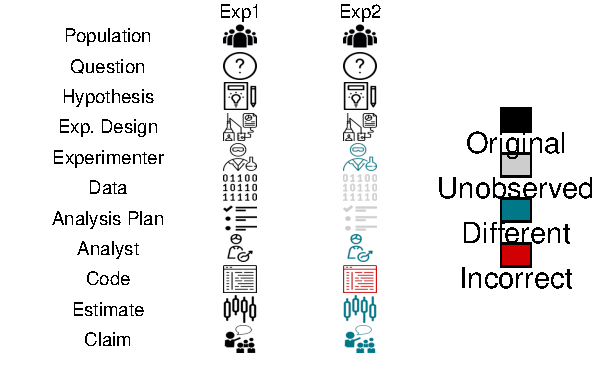
\includegraphics{sciguide_files/figure-latex/unnamed-chunk-2-1}

可重复性危机是当前科研领域里最大的问题,这里我们从空假设显著性检验(NHST)这一核心开始聊一下。NHST更常见的形式是p值,也就是在空假设成立的条件下某事件发生的概率。p值有多流行呢?根据 Jeff Leek 的\href{https://docs.google.com/presentation/d/1hzdSDaPPSE9xUYZHhOVfQIRPPdwe0A9SdE7QDsK3bOA/edit\#slide=id.g255a5ace66_3_796}{估计},如果把p值当成一篇文献,那么其被引次数已经超过300万次了,当之无愧的史上被引次数之王,甩\href{http://www.nature.com/news/the-top-100-papers-1.16224}{第二名}一个数量级。原因其实很简单,p值已经渗透到几乎所有学科的研究中了,特别是实验学科。可想而知,如果产生p值的 NHST 出了问题其影响力有多大。

如果一个假设对另一个假设来说很稀少,NHST会在很低的条件概率下拒绝掉,然后那些稀少的事情在NHST里就成了无法被检验的事情。这个例子最早是 Cohen \href{http://ist-socrates.berkeley.edu/~maccoun/PP279_Cohen1.pdf}{提出}用来说明人们在使用NHST时的问题。空假设是某人是美国人,备择假设是非美国人。我们知道某人是国会议员的概率是百万分之二,空假设里很难发生,备择假设里无法发生。空假设我们拒绝了某人是美国人,那么根据NHST,他不是美国人。但问题是议员一定要是美国人,在此类问题里,NHST永远无法认定稀有事件,也就是功效永远不足,并会给出错误答案。稀有事件总会发生,NHST总会把此类事件当成显著,即使不那么稀有,例如小概率事件如果发生了,我们就可以拒绝了。本质上是多数人在使用p值时搞混了条件概率,拿上面美国国会议员的例子来说,我们的假设 H0 在面对张三这个数据 D 时给出了拒绝 p(H0\textbar D) = 0,这个决定是构建在假设 H0 成立时出现 D 的概率太低(即p(D\textbar H0)之上,也就是说NHST下,我们默认下面的概率是成立的:
\[
p(D|H_0) = p(H_0|D)
\]
如果你修过任何基础的统计学课程都会知道这两个概率之间差了一个贝叶斯公式。通过使用贝叶斯定理,在新数据出现后原有概率是要被更新而不是直接拒绝掉的。p值给的是前者,要想知道随机生成的概率,需要知道空假设是真的的概率。通俗点说就是 NHST 属于革命派,不认可就打倒你;贝叶斯属于改良派,用新的证据更新原有理论。这个悖论的本质就是把假设下的事实与事实下的假设搞混导致的,这是NHST的一个致命问题。然而致命问题可不止这一个。

过去的100年,测量方法的精度是在不断提高的,而精度其实又会影响研究结果,很不幸,也是通过 NHST 来进行的。其实 NHST 在实验物理学里用的还是好好的,例如我去检测一个物理量,只有数据出现在其理论预测下数值四五个标准差以外才会对理论产生实质作用。此时,测量精度越高,由于测量误差导致的对原有理论的冲击就会越少,因为物理学的预测性要比化学生物等学科要好不少且此时 NHST 检测的原有理论是比较真实的。但在其他学科,特别是心理学跟医学的控制实验里,在实验开始前你几乎就可以确定空假设是不成立的,要不然你也没必要分组,此时你去搞 NHST ,几乎一定可以找到差异,此时测量精度如果不断上升,那么你会识别到一系列差异,但这些差异的效果是无法体现在p值里的,p值可能非常小,但效应却属于明显但很微弱,这样的结果也许可以发表,但对实际问题的解决几乎没有贡献。更极端的情况是如果你加大了样本量来提高统计功效,你总是能发现差异的,也就是你的空假设里原有学科理论为真也是会被方法学进步给推翻的。总结下就是 Meehl 在60年代就提出的\href{https://philpapers.org/rec/MEETIP}{悖论}:方法学的进步与增大样本数对于相对硬(理论根基深厚)的学科证伪是正面的,但对相对软(理论比较模糊)的学科则是弱化。方法学悖论的根基其实是应用学科与基础学科的矛盾,基础学科用 NHST 检验观察事实中的理论,但应用学科用 NHST 来检验的是实验设计预测下的事实,此时实验设计的那个假设与 NHST 的空假设并不对应,而 NHST 先天弱化空假设的问题就凸显了。

事实上,p值正在成为测量投资与努力而不是事实的标准,给定差异,我们总能找到足够的样本来发现这个差异(这也就是常说的功效分析)。也就是说,NHST 有时候功效不足测不到差异,有时候又一定会能测出差异,但科学事实并不会因为你使用了 NHST 而发生变化,特别是有意义的变化。而作为标准的p值其实在被样本数决定同时又综合了测定效果强度与不确定性,这样的一个标准其实有点多余,你完全可以用描述性统计与置信区间来分别表示效果强度与不确定性。p值也并不能增加新知识,考虑一个多元线性模型,我们只能在多元模型里得到参数,也就是有限检验,不能发现未知参数,但科学就是寻找未知;变量间的关系在数值改变后如何考察,正负关系如何预测,预测性也就无法实现。那么此时还有必要使用 NHST 吗?

20世纪的技术有了意义深远的进步,但更现实的问题是,科研里低垂果实已经没有了,学科从分立走向交叉,服务社会职能的出现要求科学家回答的不再是科学问题而是现实问题,或者说,科学地回答现实问题。但现实问题非常复杂,科学家要想排除影响,大都采用控制实验与随机化来验证观察研究中的事实。注意,这里的事实不再是理论假设,而是一个现象,如果本来就观察到了差异,用 NHST 根本就不会让我们知道更多的事实,我们可以用无数独立手段证明这个事实的存在然后整合进学科知识体系,但并不能产生更多的思考,理论的预测效能在 NHST 里实际是体现不出来的。而预测效果不显著在NHST里还不能说明效果不存在,到这里 NHST 基本就成了鸡肋。p值还被少数人认为结果的可重复性,但重复性是统计功效的函数,跟p值无关,p值不能传达真实与否的信息。统计功效很重要,跟样本数关系大当样本数增大时,空检验总会被拒绝,因此当空假设为感兴趣的理论时,样本数与准确性会提高理论强度,但空假设不存在时,样本数与准确性提高只会弱化理论。此外,p值控制只考虑假阳性而不是假阴性,所以对假阴性有要求的实验也要慎重使用p值。

那么我们的控制实验里对无关因素的平衡与随机如何呢?显然,平衡掉不随机的部分需要你事先知道这部分是什么,很遗憾,目前科研特别是基于观察的研究并不能事先知道,有时候就是想发现这些不知道自己不知道的东西。这种情况下基于p值或空假设的假设检验其实是不应该用的,打个比方,你发现观测数据中A基因与甲疾病相关,但究竟是不是A基因引发甲疾病还是需要用控制变量来验证的,很有可能A基因与甲疾病同样被B基因调控,但你根本就没测B基因,所以研究本身就是不完整的。

那么通过组学技术知道的不知道的我一起去测不就完整了吗?也不是,当你测量数量增加时,假设检验的个数也增加了,此时你的p值阈值如果是0.05,那么10000个测量变量中会有500个即使随机测定都会出现差异的基因。去年有人建议把p值阈值设到0.005,但p值这个问题,重要的不是把0.05降到0.005,通用阈值这个想法太偷懒,应该让研究人员充分理解p值实际意义与使用方法,毕竟在有些研究领域控制错误发现率后阈值实际比0.005\href{http://www.nature.com/news/one-size-fits-all-threshold-for-p-values-under-fire-1.22625}{低得多},改变阈值只是把需要核实的数量减少了,虽然这也有一定意义。举个例子,10000个基因中有一个是真实的,你测定后按照0.05发现了501个,按照0.005发现了51个,也就是说需要验证的数量减少了。但真实研究中,你会遇到0.05发现了501个但0.005只发现了50个的情况,真实差异由于效应量或造成的差异量不够大而被你的决策方法给漏掉了。甚至也会出现0.05发现了480个而0.005只发现了48个的情况。也就是说,当你观察的问题效应不大时,p值有可能不管怎么调整都无法发现。这个锅不在p值,在于你要研究的效应效应太低而你用了不恰当的研究方法与假设来检验这个现象。这类效应大小问题就是 type M 型错误,只要你假设检验很多,这个问题就很难规避。

同时,当你进行条件控制时,其实又掉到了高维诅咒的坑里。打比方我做了一组实验,最后发现某种药在A条件B参数面对C人群中D年龄分组里是有效的。那么问题来了,假设ABCD全是互斥的二元变量,那么我这个结果实际上是做了\(2^4 = 16\)次对比得到了一次显著性结果。然而,如果我们采用p值,那么16次随机假设检验里出现一次p值小于0.05的概率是\(1-(1-0.05)^{16} = 0.56\),也就是说这个结果在完全随机状态下也有一半可能发生。那么这个结论是否可靠呢?其实跟p值没关系,最终是跟样本量挂钩,如果你的满足条件的目标样本很大,那这个结果很可能就是对的。相反,如果这个结果是来自于小样本,虽然根据多元模型是显著的,但具体到这个条件下其实就几个样本,此时结果就不能算靠谱。探索性数据分析通常会面对这个无穷假设困境,当你不断引入协变量后,维度的增加导致样本实际是稀疏欠拟合的,最后看到现象可能就是假象。发现的价值在这里也不依赖p值,依赖效果大小与参数,进一步依赖样本量。不过条件控制中也要考虑因果关系,否则单纯增加特征值可能并不好提高模型的性能。高维诅咒实际还连着多重比较的坑,多次比较后p值是可以校正后继续用的,不过这里套的坑是无穷假设,也就是说当你比较的次数多时,有效应也看不出来了,这就要求对数据本身的结构有深入了解。当前在错误率控制上也有很多校正方法,当然也是对p值的校正,所以批评声从来也没断过。

现在只能相信强结论,也就是说无论你用哪种统计方法去进行检验,这个现象都是客观存在的,不会因为决策方法的变化而出现结论差异。不过这个提法现在看还是太理想了,因为强结论真的很强或显而易见,属于科研里低垂的果实,前人都摘的差不多了。如果一个现象足够强,p值一定会发现,贝叶斯方法也一定会发现,此时不存在效应大小问题。但更多的事实或规律是埋藏在当前认为的随机或噪音之中的,我们的分析水平也就刚刚好能把疑似信号与噪音进行区分,而这个区分是否靠谱则完全成了迷,统计学在这里帮不上忙,技术进步倒成了关键。我看到一些研究寄希望于数据挖掘技术解决学科内现象发现问题,这里我只能说对于显而易见但被忽视的现象是有帮助的,但对于高噪音数据,降低测量噪音对结论的帮助要远大于遴选能发现差异统计方法的努力。数据迷信会让你看到伪规律,而测量技术进步才会真的发现价值规律。

NHST的另一个问题在于其本身表示不了效应的方向。p值经常是双边概率取中间那一部分,所以当你看到一个很小的p值时,你并不知道这个效应的方向是更大还是更小,此时你还是需要去看效应值。在这个情况下,如果报导p值不报道效应,那么就好比我告诉你明天要变天但又不告诉你变成什么一样毫无意义。在多数实验设计中,变化几乎是一定存在的,例如我敲掉了某个基因去验证功能,基因的变化与功能肯定有区别,大都来源于观察实验,更有意义的是影响大小,这个大小更多需要专业判断而不是简单的p值。如果理科学生学了半天最后就知道用p值来判断结论,那么这个学位不给也罢。这类搞不清楚效应方向的问题是 type S 型错误,验证性实验特别需要注意。

NHST还有个问题在于p值的选择性报道或者说发表歧视,研究人员通常会尝试大量的实验条件组合但发表的论文里只有那些有显著性的结果,这导致了科研文献不科学反应研究现状。这不一定意味着结果是错的,如果这个实验条件具有广泛的数据支持而不是仅仅来自于模型推断的选择性报道,那么我们只能说推理上不严谨。不过,从这里我们可以看出,依赖p值来判断结果是存在问题的,而不使用p值,很多研究结果实际是无法简单报道的。然而,大量选择性报道可能出现一个副作用,论文的讨论很多是依赖引文,如果引文结果不靠谱,那么后续研究只有同样采用了选择性报道才能继续跟进发表,最后形成一种确认偏误,这情况比想象的要常见。甚至在系统综述过程中,对确认偏误的忽略可能通过结论影响决策者,那就成了一种自我实现。应对p值的选择性报道的方法就是公开实验完整的记录或探索性数据分析的流程,这样后来者的验证会更有针对性。而且,进行综述的科学家可以通过数据的二次分析与整合来凸显那些本来由于样本量不够而忽略的现象。

另外一种隐性p值选择性报道是通过模型选择来实现的,不同的统计模型会产生不同的假设检验结果,研究人员通常只会报道那些有阳性结果的统计模型。这个非常难识别,因为统计模型通常比较复杂且研究人员有可能是先上船后买票,也就是先发现这个模型结果有利然后根据模型组织文章。这里面会牵扯到探索性数据分析与论证的差异,如果研究人员把新模型当成了文章亮点,那读者是完全看不出来这里面的不恰当行为的。此时还是要依赖数据公开,如果大家都能下载到数据,标准化后然后同时跑多个模型,只有共存结果才有可能可靠。不过,这里面的问题在于多个模型的假设是不一样的,只有符合数据本身统计特征的模型才能被加入到评价体系里。

关于 NHST 虽然问题一大把,但系统去看,p值也有着自己的生命力,我想更多人关心的是如果我不用 NHST ,拿什么证明我的结果可靠?如果没得选,这剂毒药还是得吃啊。答案其实上面都大概提到了,你如果坚持使用p值,那么就也请同时报告参数估计与置信区间,虽然这个方法也被人喷过。如果你打算完全开一条新路,那就去学贝叶斯统计,贝叶斯统计有自己成套的处理体系,简单说就是先假设参数分布,然后用数据更新分布,后验分布计算出来就同时有点估计跟方差估计,同时多重比较问题也不存在,但随机错误无法避免,此时参数估计方差大也能体现,后续研究可以使用这次的后验数据作为下次先验数据,这样你可以实现完全的 N + 1 模式科研,其验证与预测性也很大程度依赖采样与模拟技术,之前贝叶斯方法不能流行很重要的一个原因就在于计算比较贵,现在就便宜很多了。

NHST其实是科研可重复性危机的核心,但科学家的人性也不可忽视。科学本身是构建在错误校正过程上的,但科学家评价却是人性化的,良好的评价很多时候成了科学家追求的标的。不论是对影响因子的追求还是学术明星的打造,非科学的评价与评优其实影响到了科研结果的报道。科学家正在作为一个团体来维护自己的利益与社会地位,其副作用就是对失败的低容忍度,年龄限制与成果限制使得探索必须要符合效率原则,很多年轻人在年富力强的时候做了大量排列组合而非探索性的工作来确保个人的生存无虞,这样造成的损失目前我们无法衡量。随之伴生的学术不规范、不端与造假则是层出不穷,很多人开始利用一些规则上的漏洞来实现非科研目的,例如审稿流程与评优。科学家的形象要由团体的文化来体现,阳光底下没有新鲜事,除了开放获取的研究成果,研究整体流程也应该实现透明化,这样可以很大程度防止暗箱操作。

所谓流程透明,指的是从基金申请到修改到进度报告到结题报告到文章的投稿接受与后续跟进研究及评优都要有公开的记录可以查询,文书都要经过版本控制方便返溯,所有研究人员都要实名负责对应的项目。学术团体接受公众舆论监督与同行监督,日常学术交流也要有公开的记录与反馈机制,所有的记录不直接对外公开但接受实名查询并留存查询记录。这样透明化的流程可以保证学术团体除了发表论文之外还有其他的结果展示途径,进而避免实验结果的选择性汇报与资源的过度集中。打破自我包装与人脉对科研的束缚,让结果更直白地展示给所有人。此外,关于可重复性,nature就近年来的科研可重复性危机采访了五组科学家,分别从认知、NHST、FDR、数据共享与范式转化的角度进行了\href{https://www.nature.com/articles/d41586-017-07522-z}{论述},值得一读。在医疗领域也有了一些有意思的讨论,例如认为基于人群的归纳式诊断会被个性化精准医疗所替代,此时可重复性里内含的平均律就会被彻底颠覆,分子水平的因果逻辑可能成为未来的主要知识探索方向。预印本、开放获取与审稿、科研社交媒体及数据共享等新\href{https://theoreticalecology.wordpress.com/2019/01/22/tree-species-richness-and-its-effects-on-productivity-neither-global-nor-consistent/}{趋势}也孕育着新的问题解决方法。

这次的危机能不能解决?什么时候解决?现在谁也不知道,但了解问题是解决问题的第一步,而路还很长。

\hypertarget{ux79d1ux5b66ux95eeux9898}{%
\section{科学问题}\label{ux79d1ux5b66ux95eeux9898}}

2005年《科学》杂志提出了100个科学\href{https://science.sciencemag.org/content/309/5731/78.2}{问题}。目前国家关心的科学问题由中国科协筹集,每年发布。

\begin{itemize}
\tightlist
\item
  超高精度量子惯性导航技术
\item
  空间天气的及时准确预报
\item
  岩石圈构造应力场及其作用过程
\item
  煤矿重特大灾害智能报警方法与技术
\item
  工程结构安全的长期智能监测预警技术
\item
  城市交通基础设施智能协同运营技术
\item
  基于北斗卫星和5G通信技术的新型高速铁路列车运行控制技术
\item
  高原高寒冻土地区高速铁路与公路修建关键技术
\item
  跨深大海峡通道(悬浮隧道)关键技术
\item
  面向未来交通的路网全感知技术
\item
  时速1000公里及以上低真空管道运输高速磁悬浮铁路建造关键技术
\item
  未来城市地下交通及物流系统
\item
  航天运输技术难题
\item
  飞机级系统架构设计及仿真技术
\item
  面向工程应用的高精度动态测量
\item
  高效长寿命低成本电化学电力储能技术
\item
  海洋生态系统储碳与全球变化
\item
  脆弱生境生物多样性的维持机制
\item
  高水平放射性废物安全处置
\item
  绿色安全高效的低成本制氢技术
\item
  川藏铁路建设难点
\item
  未来全球能源互联网的关键技术
\item
  绿色农药创新研究和原创性靶标的发现
\item
  固态有机废弃物生物转化及其资源梯级利用
\item
  植物工厂人工环境条件下植物的生长发育调控
\item
  基于核酸物质的基因精准调控与医药技术
\item
  细胞命运决定机制的研究
\item
  人类智能的基因调控机理
\item
  全球变化对动物的影响及应对
\item
  植物对逆境的记忆功能与进化
\item
  DNA存储技术
\item
  意识读取的前沿问题和关键技术
\item
  遗传信息的结构编码------纳米尺度遗传信息动态结构解析
\item
  记忆的物理化学基础
\item
  单分子化学反应动态过程的可视化
\item
  超临界场强的量子电动力学效应
\item
  宇宙中重元素的起源
\item
  极端条件下的可控燃烧
\item
  高性能热电材料
\item
  纳米纤维的产业化生产关键技术
\item
  核能系统高安全结构材料
\item
  高活性可见光催化材料
\item
  人工智能技术与新型智能复合材料的深度融合
\item
  类脑计算
\item
  新一代认知物联网关键技术
\item
  抗量子密码算法设计
\item
  大规模共享无人载运工具的协同智动管控仿真
\item
  工业互联网中数据集成和边缘处理技术
\item
  人与机器的情感交互
\item
  肿瘤转移机制与抗肿瘤转移新药研发
\item
  老年性痴呆的机制解析及诊治难点
\item
  精神疾病的新型治疗方法
\item
  免疫微环境分子分型及免疫治疗耐药机制
\item
  人机共融关键技术
\item
  微腔中的力光量子传感
\item
  高性能动力电池研发技术
\item
  新一代智能制造系统
\item
  基于多源信息融合的大型复杂系统健康状态监测与评估
\item
  人工智能在智能驾驶工程技术开发中的应用
\item
  先进微纳机器人技术
\item
  暗物质是种能探测到的基本粒子吗
\item
  对激光核聚变新途径的探索
\item
  单原子催化剂的催化反应机理
\item
  高能量密度动力电池材料电化学
\item
  情绪意识的产生根源
\item
  细胞器之间的相互作用
\item
  单细胞多组学技术
\item
  废弃物资源生态安全利用技术集成
\item
  全智能化植物工厂关键技术难题
\item
  近地小天体调查、防御与开发问题
\item
  大地震机制及其物理预测方法
\item
  原创药物靶标发现的新途径与新方法
\item
  中医药临床疗效评价创新方法与技术
\item
  人工智能系统的智能生成机理
\item
  氢燃料电池动力系统
\item
  可再生合成燃料
\item
  绿色超声速民机设计技术
\item
  重复使用航天运输系统设计与评估技术
\item
  千米级深竖井全断面掘进技术
\item
  海洋天然气水合物和油气一体化勘探开发机理和关键工程技术
  冠状病毒跨种传播的生态学机制是什么?
\item
  引力波将如何揭示宇宙奥秘?
\item
  地球物质是如何演化与循环的?
\item
  第五代核能系统会是什么样子?
\item
  特种能场辅助制造的科学原理是什么?
\item
  数字交通基础设施如何推动自动驾驶与车路协同发展?
\item
  调节人体免疫功能的中医药机制是什么?
\item
  植物无融合生殖的生物学基础是什么?
\item
  如何优化变化环境下我国水资源承载力,实现健康的区域水平衡状态?
\item
  如何建立虚拟孪生理论和技术基础并开展示范应用?
  如何开发新型免疫细胞在肿瘤治疗中的新途径与新技术?
\item
  水平起降组合动力运载器一体化设计为何成为空天技术新焦点?
\item
  如何实现农业重大入侵生物的前瞻性风险预警和实时控制?
\item
  信息化条件下国家关键基础设施如何防范重大电磁威胁?
\item
  硅光技术能否促成光电子和微电子的融合?
\item
  如何解决集成电路制造工艺中缺陷在线检测难题?
\item
  无人车如何实现在卫星不可用条件下的高精度智能导航?
\item
  如何在可再生能源规模化电解水制氢生产中实现``大规模''``低能耗''``高稳定性''三者的统一?
\item
  如何突破进藏高速公路智能建造及工程健康保障技术?
\item
  如何突破光刻技术难题?
\end{itemize}

\hypertarget{ux65b0ux5174ux5b66ux79d1}{%
\subsection{新兴学科}\label{ux65b0ux5174ux5b66ux79d1}}

\begin{itemize}
\tightlist
\item
  纳米材料
\item
  表观遗传学
\item
  基因修饰技术
\item
  测序技术
\item
  蛋白质结晶
\item
  组学
\item
  量子计算机
\item
  区块链
\item
  数据科学
\item
  深度学习
\item
  虚拟现实
\item
  增强现实
\item
  干细胞
\item
  气候变化
\item
  3D打印
\item
  生物入侵
\item
  物联网
\item
  可穿戴设备
\item
  无人驾驶
\end{itemize}

\hypertarget{ux70edux70b9ux5b66ux79d1}{%
\subsection{热点学科}\label{ux70edux70b9ux5b66ux79d1}}

\begin{itemize}
\tightlist
\item
  复杂性科学
\item
  脑科学
\item
  癌症
\item
  心脑血管疾病
\item
  老龄化
\item
  分析化学
\item
  材料科学
\item
  新能源
\item
  催化
\item
  全合成
\item
  育种
\item
  生物信息学
\item
  人工智能
\item
  机器人
\item
  进化
\item
  宇宙
\item
  地质
\item
  传染病
\end{itemize}

\hypertarget{ux804cux4e1aux5b66ux79d1}{%
\subsection{职业学科}\label{ux804cux4e1aux5b66ux79d1}}

\begin{itemize}
\tightlist
\item
  医学
\item
  会计
\item
  法律
\item
  工程学
\item
  建筑
\item
  计算机科学
\item
  统计学
\item
  金融
\item
  护理
\item
  营养
\item
  工商管理
\end{itemize}

\hypertarget{ux901aux8bc6ux5b66ux79d1}{%
\subsection{通识学科}\label{ux901aux8bc6ux5b66ux79d1}}

\begin{itemize}
\tightlist
\item
  博弈论
\item
  心理学
\item
  历史
\item
  文学
\item
  艺术
\item
  哲学
\item
  地理
\item
  外语
\end{itemize}

\hypertarget{thought}{%
\chapter{思维工具篇}\label{thought}}

\hypertarget{ux79d1ux5b66ux601dux7ef4}{%
\section{科学思维}\label{ux79d1ux5b66ux601dux7ef4}}

这里会侧重科学研究中比较重要的思维工具,但绝大多数讨论还是来自科学哲学。虽然做科研一般都不讨论哲学,太多形而上的东西,说也说不清道也道不明还无法证伪。但懂一点科学哲学还是很有必要的,不然很容易研究着研究着就会觉得自己做的东西是垃圾,是谋生的工具,虽然从某个角度看也没错,但科学哲学无疑是应对这种心态最好的老鸭汤。

首先,哲学是解决人与世界关系的学问,而科学在词源(scientia)上是知识学问的意思,追求的是正确的东西或真理。哲学很多时候与哲学史等同,提的问题几乎万古长存,各流派解读的保质期也很久甚至就不存在伪的可能。科学跟科学史就完全不同,是一种探索自然的理性精神,很多知识会被更新,了解科学史会更博学但并不增加科学知识本身,因为对于一件事科学上的描述几乎唯一。当我们认为自然是可知的时候,科学就是探索其原因原理的认识方式并提供方法工具。

科学方法论构建于三个基础之上:观察或实验、数学还有逻辑工具。观察与实验要做到可重复、可比及随机;数学提供量化评价工具;逻辑工具包括不限于归纳演绎、分类类比、公理化及假说演绎。科学提供的一定是系统性规律性的知识,任何学科如果没有自己的理论系统、数学模型与验证都只能算知识或经验,谈不上科学化。科学哲学主要关注哲学史里跟科学相关的世界观、认识论与方法论。

\hypertarget{ux53e4ux5e0cux814a}{%
\subsection{古希腊}\label{ux53e4ux5e0cux814a}}

哲学是爱智慧这个梗就不多说了,扯古希腊也显得俗套,反正有了古希腊人才有了理性跟逻辑的提法。古希腊前面的历史可理解成经验性知识的发展,知识多了就要有规律总结出来,逻辑和理性可看作用来生成规律的知识。其实哲学就是认识世界的知识,泰勒斯有一套,毕达哥拉斯有一套,赫拉克里特有一套\ldots\ldots 大家能自圆其说就来一套,对不对另说,不服就辩论,赢了就是真理,输了就是谬误。逻辑与理性最早就出自于这些街头巷尾的辩论,两套理论对比,总得有两方都认可的法则才有结果,理性或许就是这种普遍性知识的产物。

不过辩论有诡辩这一说的,苏格拉底看不下去了就说你们这些人都觉得自己对,但有可能是不对的,反正我自知我无知(这句是我认可最有智慧含量的句子,还有一句:天下没有免费的午餐)。苏格拉底不怎么关注解释万物,有点回归个人或社会的意思。到了柏拉图直接就理想国了,世界形物均为理型的影子。再到了亚里士多德就不怎么废话了,直接取消理型世界的存在,认为万物有因,这个因就是所有问题的因,寻找到最终因,真理就明了了。亚里士多德这个看法后来发展成第一推动问题,宗教界觉得只有全能的主有这能耐,就把亚里士多德的理论吸引到宗教哲学里去了。

同时,我们现在所提到的科学源于日本,可理解为分类的知识,而最早对人类知识体系分类的就是亚里士多德。他还很神奇的将自己的目的论揉到这个分类里去了,亚里士多德分类体系很完整,能解释的东西很多,所以后来几百年大家就都用了这个体系。其实这时候科学知识更适合分到亚里士多德所谓的自然哲学这个科目里,这个科目特指自然现象的规律及探索方法。这里需要注明的是数学更多是工具,数学化不一定就代表科学,另一个需要注意的是逻辑学,亚里士多德的三段论十分精彩,以至于要不是后来哥德尔横空出世,任谁也动不了根基。

\hypertarget{ux4e2dux4e16ux7eaa}{%
\subsection{中世纪}\label{ux4e2dux4e16ux7eaa}}

中世纪黑暗吗?如果看天气应该跟现在差不多,但这个黑暗的印象大致源于天主教对知识的垄断,而知识也反过来服务宗教,而宗教理性在一定程度上促进了我们对世界的认识,所以盲目对立宗教跟科学没必要,很多前期知识都是不少富有宗教热情的理性人士总结的。只不过知识很多种,科学在那年代连个独立的名字都没有,大体可以分为偏形而上学的自然哲学与偏事实的博物学,所以你看,牛顿写本书叫《自然哲学的数学原理》,跟现代意义上的科学没啥关系,所以你管他信仰什么呢,而博物学的英文是 nature history,只是后来伴随各学科发展基本都理论化为专门的学科了。这个时候,科学知识跟形而上学还是分不开,很多知识有严谨的数学形式但你无法证实,很多天文学知识就这德行,你去看看托勒密体系,圆环套圆环的也能解释现象,那哥白尼的日心说为什么就流行了呢?因为是真理?因为结构简单?还是因为他用了别人看不懂的语言写出来的?或者说反对者死绝了新理论就流行了?总之,没有实证的理论的流行不会是你想的那么简单,但一般来说,人们都喜欢简单且解释面广的理论,宗教也这样,毕竟他们认为美的东西都是上帝赐予的。值得注意的是这种简单为上的奥卡姆剃刀原理就是中世纪末神学家提出的,现在也经常被科研工作者提起。在科学这个提法之前,用一套知识来解释世界是各代学者所向往的,才不管验证什么的,理性重于事实。

中世纪产生了奥古斯都的教父哲学,吸收了柏拉图主义,认为理性要服从信仰,上帝只能信仰,不能认识。其后出现的经院哲学(代表人物托马斯·阿奎纳)则更多吸收了亚里士多德的思想,认为理性有助于信仰,认识提供了客观性。不过总的来说,中世纪神学成了唯一的学问与意识形态。学者吸收了古希腊哲学中形而上的部分,但对于探索自然与事物规律兴趣不大,更多放在神学经典的理论化抽象化上,例如针尖站多少天使的讨论之类,虽然也算理论问题,但对改善生活质量意义不大。

\hypertarget{ux6587ux827aux590dux5174ux4e4bux540e}{%
\subsection{文艺复兴之后}\label{ux6587ux827aux590dux5174ux4e4bux540e}}

历史的发展是伴随知识的增长的。大航海时代为人类的知识提供了一个海量来源,文艺复兴带来了人性的解放,宗教改革让生活走出了政教合一,总之,经验开始比逻辑更为人接受。英国的培根开创近代唯物论与经验论学派,提出实验是获取知识的途径,打击了经院哲学过分看重逻辑与教义而不重视现实事物的观点;而欧洲大陆的笛卡尔则开创了二元论,创立唯理论学派,其基本出发点在于如果你的存在只因为你思考与怀疑才会出现,不思考啥都不存在,所以思考就是第一推动,依赖感知世界的经验不如理性思考更接近上帝,在这里笛卡尔反对的是经院哲学里对教条的推崇,主张怀疑与思考。

虽然这两派都是反对经院哲学,但却开启了欧洲大陆的唯理论与英国的经验论的争执,争论核心在知识的构建是从理性出发还是从经验出发,这两种观点打架几百年。在经验论学者看来,经验是一切知识的来源,感性认识很重要,归纳很重要。培根的继承者霍布斯基于伽利略的力学提出了机械唯物主义。洛克则制定了经验论的认知论体系。发展到巴克莱就成了``存在就是被感知'',再往后到了休谟则发展成了彻底的怀疑论,他批判归纳方法论的循环论证,认为除了感觉什么都不可知,终结了古典经验论。而唯理论学者则认为理性来自于自明之理,可以把握事物本质,只有理性推导或演绎出来的知识才可靠。斯宾诺莎则强调了伦理道德的意义,提出几何学考察自然、心灵与情感。莱布尼茨则批判了洛克的经验论,系统化了唯理论。

到了康德的时代后,综合经验论与唯理论就很重要了。知识需要有普遍性且可以发现新内容,分析可以解释事物而综合可以把经验扩充。这样我们就需要一个科学可以成立的认知根基,一个逻辑分析可以立足且给经验扩充空间的基础认知概念。康德认为先天综合判断就是这样的根基,人的认识活动既不单纯是经验也不单纯是概念,本质是认识主体对经验概念的运用,在这个过程中依赖先天知识形成认识对象,也形成普遍必然知识。

那么什么是先天知识?可以理解为感性直观或数学,时间、空间是先天的,也是数学对象本质,时空先验保证了感觉的客观性与经验的实在性,感性世界能感知到的现象背后存在物自体。那么我们如何获得知识,需要知性或抽象能力,感性给了我们直观材料,而知性通过概念思维对象来形成具有普遍有效性的知识,从感性与知性结合角度康德提出先验逻辑,区别于只关注形式的形式逻辑,先验逻辑看重内容。而知性理论的综合就是理性,无条件、绝对、完整的东西。理性可以把知性推广到经验之外,是可以超越经验的。科学研究活跃在感性与知性之间,科学知识就是先天综合判断的结果,但物自体与绝对理性都不在科研范围之内。黑格尔在其后认为主体客体应该是辩证统一的,绝对精神统一一切,不过科学在黑格尔体系里就没什么科学,概念成了一切本原,无穷的辩证统一滚滚向前。在黑格尔哲学体系里部是自洽且不可证伪的,但很多宗教理论也是类似的,为了保证理论完整性而抛弃事实验证的哲学可以被称为形而上的理论,但跟科学已经没了关系。

到了19世纪末大家都不争了,因为实证主义一统江湖认为从经验中提取逻辑,然后再证实就OK了,那些形而上的东西就不管了,此时科学哲学抛弃掉了神学的虚构与形而上学的绝对,只关心经验现象与事实及其背后规律。这时候科学哲学才独立出来,而观察式的经验也开始让位于实验式的事实,人们不满足于被动接受知识,开始主动去寻找真相。

\hypertarget{ux903bux8f91ux5b9eux8bc1ux4e3bux4e49}{%
\subsection{逻辑实证主义}\label{ux903bux8f91ux5b9eux8bc1ux4e3bux4e49}}

当人自己把握了主动权,原有的常识知识就要被逻辑重新检验,而无法检验的就划到形而上学这一类里留给做宗教神学的人去讨论。换言之,从柏拉图开始的将现实世界与理想世界的区分被打破了,原来的哲学家都醉心于构建理想世界而不关心现实生活,而逻辑实证主义则要求通过生活的事实来寻找真相。换句话,经验事实及逻辑推理被结合用在真理的探索上了。而经验事实的崛起则伴随着归纳法的崛起,事实成为知识的唯一来源,科学开始渗入并改造哲学方法论,这一转变真正让科学有了真理探寻的光环,一举扫清神秘主义与宗教束缚,直到今天还在深刻的影响着每一个科研工作者。值得一提的是,逻辑实证主义出现时正值数学遇到集合论悖论与物理学遇到两朵乌云,实验结果矛盾造成的理论危机其实是逻辑实证主义可以发展的诱因。此外,逻辑实证主义也深受马赫的新实证主义(一元论与反对力学绝对空间)、彭加莱约定论(约定是理论与经验的产物,对约定的选择自由而不任意,由经验引导)及罗素维特根斯坦的逻辑原子论(基于原子命题与事实来构造知识,哲学主题是命题的逻辑分析)影响。

逻辑实证主义是现代科学哲学中第一个也是唯一一个完整严谨的体系。石里克是主要代表人物,其主旨在于让哲学与自然科学密切联系,在新物理学而不是亚里士多德或康德体系上构建认识论与方法论。逻辑实证主义重视证实与观察,推崇可检验性,反对原因,推崇常规性与描述性,抛弃掉以太、原子、电子等理论对象,拒斥形而上学与过度思辨,强调逻辑分析方法。

但不久大家发现不对头,因为不确定什么叫做可证实,单纯基于经验如何证实全称理论?本质上就是逻辑实证主义所采用的归纳法不如演绎法严格,得到的结论有局限性,不够严谨。在逻辑实证主义阵营里,卡尔纳普注意到了证实的经验问题,改为了确证,也即是将证实卡在当前认识水平内,只要后面有新证据出现就更好进行条件确证,类似贝叶斯定理。卡尔纳普另一思想是语义分析,严格区别语言中的语义与形式,消除误解。

逻辑实证主义后期的代表人物是亨普尔,提出了科学说明理论,认为科学是用科学定律来回答为什么的问题。亨普尔强调相关性与可检验性要求,引入概率来体现归纳规律的说明力,认为定律和现象之间的演绎有效或高概率支持。不过因为反对因果强调逻辑形式分析,导致相关性在说明上的困难,在解释历史与日常事件上也显得脱离实际。

\hypertarget{ux5426ux8bc1ux4e3bux4e49}{%
\subsection{否证主义}\label{ux5426ux8bc1ux4e3bux4e49}}

面对逻辑证实主义,波普引入了更多批判性的思考。其出发点在于认为演绎法试错作为验证手段比单纯经验证实要靠谱。大家都提假说,然后验证它,出现反例就把假说否了,不能否证就不科学,这就是证伪。一时间大家都接受了,神马佛洛依德,历史唯物主义都因为自洽但不能证伪给踹出科学圈了。证伪也可理解为试错,如果连错都理论上不存在,那就肯定不是科研可以搞的,大都是循环论证。这里奥卡姆剃刀再次登场,认为越简单的理论就越容易检验,复杂如哈奇森效应的现象与理论不值得研究。

不久又有人感觉不对了,一方面演绎法很难产生新知识,另一方面貌似假说是无穷无尽了。证实比较费事,证伪容易但很多理论就垮了。为了调和这个矛盾,否证主义给出的答案是演绎法虽不能产生新知识,但假说的产生不是无缘无故的,而知识的进步应该通过大胆猜想的确证与谨慎猜想的否证来完成,一个推翻的理论必然联系着新理论的提出,这时不断发展的,而科学的任务就是处理进步问题而非回答真理问题。形而上学也并不完全被排斥了,因为假说的提出有时就是没有事实证据的。进一步讲,波普尔将世界分成世界1,也就是物理世界,世界2,也就是精神世界,然后又分了个世界3,也就是客观知识世界。这种三分法其实是将柏拉图的理型世界进化了,同时也留下了世界2的个人空间。每个世界都在进化,这就是科学发展的轨迹。一口吃不成胖子,我们就去试错吧!猜想与批判这一否证主义的核心思想也是当下科研中比较闪光与巧妙的实验设计动机来源。

\hypertarget{ux5386ux53f2ux4e3bux4e49}{%
\subsection{历史主义}\label{ux5386ux53f2ux4e3bux4e49}}

前面那些理论的提出者大都数理化出身,推理证明构建系统很在行,但没案例不成啊,得解释得了现象啊。其中一些人翻了翻了史书,发现很多发现不是通过证伪得到认可的,也不是建立在大量归纳的基础上,而是具有``历史性''。也就是逻辑不怎么灵光,然后他们就说咱以史为鉴吧!拉卡托斯就搞出了个硬核软核的理论,大意说一个理论是有生命力的,硬核部分无须质疑,有保护带,一时半会死不了。需要缝缝补补的是外围软核,什么时候硬核也不行了,就退出历史舞台了。这个解释保全了科学理论体系,也就是堵了民科的路,要知道民科最喜欢证伪,一个错误就否了整体,现在拉卡托斯说不成,得慢慢来,有历史的。理论是互相连接成一个纲领的,出现了反常并不可怕,可以理论自身发展来接纳反常。当一个纲领无法发展或出现另外的纲领可以解释更多事实时,此时会逐渐淘汰掉退化纲领,其分界标准在于对新事实的预见性。

不久又有人感觉不对了,我怎么知道现在的硬核到底对不对?拉卡托斯这时就呵呵了,交给历史评价吧!库恩在这个背景下提出了范式,他本身有较强的历史功底,手头案例多,所以有了科学共同体这个说法。大意就是一个时代的真理主流说了算,这伙人挂了而接任的更多采取了另一种解释现象更多的理论,那这个理论就上位了,就革命完成了。前面那个时期比较压抑就叫前科学,后面上位了就是常规科学。之后又有新现象解释不了了就有了危机,这时候新理论又出现了,再搞一次革命就OK了。范式是来区别前科学与常规科学的,范式通常是一套当前时代科学共同体所使用的理论体系,而这个理论体系要比之前的更能解释更多的问题也更严格。这理论比拉卡托斯那一套通俗易懂,那年代搞政治的一看有革命二字纷纷表示深有体会,大力推广之,所以范式着实火了好一段时间,不过此时理性主义已经让位于非理性主义。

库恩的范式革命是格式塔式的转换,历史上一共也没发生几次,真正有益的是他对范式定义时要求要有自称科学的学科要有自己的理论体系与假设且对现实世界产生作用,这个理论自身并不要求科学家的态度是客观的,但范式自身要是客观的。这时候,大家都不愿搭理真理性这茬了,因为都清楚对错问题是历史性的。同时范式也把形而上学彻底请回到科学体系中了并认为对科学的发展是有益的,要知道波普尔虽然不拒斥形而上学但本质还是批判形而上学的,所以历史主义的强调使得真理相对化。

\hypertarget{ux65e0ux653fux5e9cux4e3bux4e49}{%
\subsection{无政府主义}\label{ux65e0ux653fux5e9cux4e3bux4e49}}

事实上你沿着这个思路走下去发现貌似科学发展跟三国演义差不多,不在于对不对而在于认可的多不多,有没有跟你闹革命的。当然因为实证主义的余威,理性与逻辑在科学研究中是绕不开的。这时候来了个更霸气的费耶阿本德,一拍桌子,科学跟别的知识没啥区别,不能特殊对待。 后来流传到世上的就是那句 anything goes 。他信奉无政府主义,认为科学在无政府主义下比起理论上的法则与规律更鼓励进步,更极端点就成了达达主义,不对科学设定任何边界,也不坚持逻辑一元论,提倡非理性的科学观,以自由名义反对科学主义。很多人认为这货终结了科学哲学的发展。从20世纪初到六七十年代这个学科就完蛋了,这就是科学哲学的学科危机。

\hypertarget{ux5b9eux7528ux4e3bux4e49}{%
\subsection{实用主义}\label{ux5b9eux7528ux4e3bux4e49}}

逻辑委实打不过历史,原来那些搞科学哲学研究的还没死就没饭碗了,生存是硬道理。他们发挥了科学共同体的作用,把费耶阿本德斥为异类、后现代。但他说的话又绕不过去,这时候劳丹提出要回归理性,提倡进步性,而进步性应该是解决问题能力的增强,此时追求真理已经不再重要。而美国人想来想去想到了有用两个字,然后大家纷纷鼓掌。理性,历史都打不过生存这个命题。有用是硬道理,有用解释一切,然后就没有然后了。

\hypertarget{ux5176ux4ed6}{%
\subsection{其他}\label{ux5176ux4ed6}}

除此之外,由于逻辑讲求语义明确而严格,但要是日常交流用一堆符号估计谁也受不了,所以科学哲学也在语义学方面继续发展。英国人的经验论也促进了新实验主义与主观贝叶斯学派的发展,慢慢地科学哲学也开始接受一些非实在论的观点,而科学实在论是穿插在上述命题中的。

科学哲学从实证主义发展到今天,被各种新命题与发现折腾的够呛,从里面提一个片段就可以看到很多,科学是什么?它跟哲学啥关系?又对哲学发展有什么样的影响?总之,我们没有停下探索真理的脚步,答案在哪里也毫无头绪,只要不满足于现状,知识就存在进步的可能,同时须知人生苦短,自知无知是很重要的。

就科研本身而言,最开始属于观察现象然后总结规律的经验方式,后来慢慢形成学科体系与知识框架来设计实验预测解释事实,现在其实更多是逻辑与经验的混合来解决科学问题。也就是说,学科知识是基础,但问题总出在前沿也就是知识覆盖不到或部分覆盖的地方,经验论与唯理论的斗争时常出现,单纯看经验或者说观察与实验会推动问题的解决,但有时候也推不动:很多规律不一定经得起检验,还有很多规律需要的限定条件太多进而导致应用上矫枉过正,还有些学科提出规律本身产生的反馈会导致规律失效(也就是反身性,在观察研究学科中比较多)\ldots 规律不代表真相,只是事实的一种描述,所有规律都要接受且长期接受事实检验,直到被描述更精确全面的规律取代。科学靠谱很大程度是规律性进行的保障,规律保证了可预测性,但其实很多规律描述同一问题的话恰恰说明这个问题很复杂,没有简单规律。规律要有数学背书才会严格,但数学本身不代表科学。规律间互相支撑就可以构建学科的知识体系,如果一个学科没有被广泛认可的规律,那么共识就无法建立。

\hypertarget{ux6570ux5b66ux601dux7ef4}{%
\section{数学思维}\label{ux6570ux5b66ux601dux7ef4}}

数学是关于数量关系与空间形式的学科,是数与形的学问,核心是培养数学思维。数学思维主要是证明与计算,前者锻炼逻辑推演思维,特别是基于公理体系的推演,后者锻炼计算与算法构造思维。数学不是科学学科但为科学提供思维与工具,无法数学化的科学知识很难独立为一门学科。

数学早期有很强的实用目的,例如计数与算术,古希腊时期逐渐过渡到几何公理体系。古希腊数学代表人物有泰勒斯(半圆直角定理)、毕达哥拉斯(万物皆数、黄金分割、无理数)。在雅典时期出现了芝诺(无限概念)、巧辨学派的三大作图问题(立方倍积、化圆为方、三等分角)、雅典学院(不懂几何莫入)与吕园学派(亚里士多德三段论)。到了亚历山大时期,欧几里得写出了《几何原本》,给出了世界上第一个公理体系。阿基米德提出类似积分的平衡法。后来中世纪降临,女数学家希帕蒂亚之死与亚历山大图书馆被焚标志着希腊数学的终止。

古代中国用图形数字标示规律是河图洛书。《墨经》里也出现了理论思辨的萌芽。《周髀算经》与《九章算术》是早期的数学经典,涉及了负数、无理数、方程术等概念。几何上赵爽弦图给出了勾股定理的证明,刘徽提出割圆术,祖冲之计算了较为精确的圆周率,虽然其学术作品《缀术》失传了。宋元期间有贾宪三角与正负开方术、秦九韶的大衍求一术、沈括内插法、天元术及四元术等。印度早期有巴克沙利手稿而阿拉伯世界大力发展了代数学并翻译了大量古希腊经典。数学知识伴随贸易与战争从各文明起源地逐渐汇拢到了西欧。

文艺复兴时期,斐波那契写了《算经》,介绍了印度-阿拉伯计数法。韦达的《分析引论》确定了代数符号体系与代数运算。绘画发展促进了透视与立体几何的研究。到了笛卡尔,他注意到几何与代数无法互补,同时经院哲学无法发现新知识,进而在《几何学》提出了通用数学的概念,首先把任何问题都抽象成数学问题,然后数学问题代数化,联立方程求解,求解过程用几何方法辅助。

到了大航海时代,贸易与航海的需求让很多计算问题有了实际的对应,例如瞬时速度、切线、函数极值、重心引力计算等。在此基础上,微积分的发明就尤为重要,牛顿跟莱布尼茨的优先权之争背后是英国经验主义与欧洲大陆理性主义的借鸡下蛋。然后达朗贝尔、欧拉、拉格朗日等进一步严格化微积分。后来偏微分方程论与微积分的共同发展形成了现在的分析学。不过,在18世纪末出现了悲观主义,认为数学到分析学只剩下细枝末节了。

不过19世纪,代数学又开始了新发展,从研究方程和具体的数到了抽象集合的运算规律,开了新天地。几何学也不在纠结第五公设,直接进入非欧几何的新世界,高斯功不可没。后来,几何学统一到了克莱因埃尔朗根纲领下,成为研究几何图形对于某类变换群保持不变的性质的学问。人们对几何的认识,从三维到高维,从平面到弯曲,从刚性到影射,只要数理逻辑上成立,皆可研究。到了19世纪末,除了集合论相容性问题,分析的严格化几乎完成。

进入二十世纪,希尔伯特公理化方法尝试了更高更基础的统一性。在此基础上,出现了纯数学、泛函分析、抽象代数、拓扑学、概率论、动力系统、随机过程、代数几何等研究方向。不过,集合论悖论及哥德尔不完全性定理给了数理逻辑进一步发展的可能。这个时期的主要进展有两个,一个是数学难题的攻克,另一个则是应用数学空前繁荣,渗透到了几乎所有知识领域。应用学科中,数理统计、运筹学、控制论、博弈论、计算机科学等都算是相对独立的学科了。数学自身正在致力于解决难题,相当一部分难题是纯粹抽象的,跟科学关系不大了。然而,科学正在不断整合借用数学工具与思维,探索世界的规律。

数学的学科发展跟科学有密切关系但本质是不一样的。科学是要做真假判断与验证的,哪怕知道这会被推翻。数学则有自己相对完备的逻辑世界,可以做到一定程度的纯公理演绎。数学基础理论无法证伪而科学理论一定存在被推翻的可能,被数学化的科学如果无法与事实接轨只能被看作假说,例如弦论就存在逻辑自洽的多个版本。科学是一个不断发展的过程,需要实验与观察来更新自己,数学可以不依赖这些。

\hypertarget{ux7edfux8ba1ux601dux7ef4}{%
\section{统计思维}\label{ux7edfux8ba1ux601dux7ef4}}

统计思维包括但不限于抽象、似然度、回归、因果、残差等。这里推荐《统计七支柱》、《为什么》与《女士品茶》作为统计思维的理解读物。统计思维可能是科研中最重要的一部分,更多数据分析内容见第五章。

\hypertarget{ux62bdux8c61}{%
\subsection{抽象}\label{ux62bdux8c61}}

最原始的统计需求就是对客观世界的抽象,跟农业最相关的天文观察要求所有测量要准确,但问题每次测出来都会有差异,那么就需要一个方法来描述相似但不一样的测量值,这就是统计聚合思想的来源。科幻小说中有照相机记忆的人是无法分析事物的,他们只能记住所有细节,而这个负担是非常重的,此时抽象的意义就很大了。所谓大数据就好比这个人,细节丰富但需要抽象,不然就是一堆数字的堆砌。这里最常见的统计学术语就是众数、中位数还有均值,都是聚合抽象描述的体现。

创立统计量是第一步,需要背景知识的辅助与对数据本身分布的描述。数据分布是非常基础的统计量构建工具。例如正态分布是随机数的集合;对数正态分布是随机数乘积的分布,为正数,单对数坐标轴是正态分布;幂律分布是出现在双对数坐标轴的直线,产生于优先连接模型或马太效应,另一种解释是自组织临界现象,例如林火模型等灾难的积蓄发生,社交从众增加了不平等,更多机会尝试会有更大方差结果出来等等。背景知识是对分布的逻辑解释,这对预测或工程应用也许意义不大,但科研需要知道为什么。

当我们形成一个统计量,其实是丢掉了一些信息的,但更有意思的是对同一个事物的描述,即便测量的准确性上没有差别,后来的观察贡献的信息并不如早期多,信息量与观测数的开方正比而不是观测数。举例来说,早期造币按批次称重,误差r,10个一起称的误差就并不是10r,100个一起称也不是100r,你称10个得到的误差与称100个得到的误差精度最多高一倍,也就是后面90个硬币提供的信息大概等同于前10个提供的信息,这个现象也是统计学里很常见的,基于此我们可以去搞采样及基于分布的理论而不至于担心丢失太多信息。

在分布属性中,方差值得特别关注,因为方差体现了数据的变动或者说异质性,而数据的变动直接影响结论的可靠性。方差分析的核心思想就是检验数据的异质性,看你设计的分类是否让组内是均质的而组间是异质的,如果我们方差分析做的足够好,应该可以把整体数据拆成一个个可解释的符合数学描述的分布。同时方差作为衡量变动区间的一个指标对于风险控制与区间估计也很有意义,关注方差就比只看单一描述提取更多的信息。

\hypertarget{ux4f3cux7136ux5ea6}{%
\subsection{似然度}\label{ux4f3cux7136ux5ea6}}

另一个统计思想是似然度,有了测量就可以进行比较,最通常的比较就是跟随机事件比,有了随机事件就可以谈概率了。此时特定分布下概率就是似然度,看看某件事在大背景下出现的可能。p值理论的根基就是似然度概率且最初的p值概念里就是仅仅去看空假设下的发生概率。1920年Fisher提出,如果A代表科学目标,X代表数据,那么定义似然度函数L(A\textbar X)为出现X的A的概率密度函数,X已知,找这个函数最大时的A,一阶导数为0找到参数,二阶导数描述准确性,但这里面最大的问题在于对于方差估计是有偏的,特别是数量少时,而维度高了这个问题就很严重了。

抛开这个,基于概率的推理本身就是统计学很特殊的世界观,简单说就是只要概率不为零,一切皆可能。休谟认为奇迹是违反自然法则不能发生的,但 Price 用贝叶斯理论推导认为即使发生概率很小,多次实验后也会发生奇迹,在这里经验法则跟统计规律就出现了对立。传统世界观是决定论的、逻辑的,但统计世界观是概率的,不可知的或可更新的,值得注意的是,这种不可调和的差异也存在与量子力学与经典力学的世界观之间。很难说那种是世界本来面目,只能说这是两种认知角度,可以矛盾地存在于同一个人身上。

有了面向背景目标的似然度,统计学可以解决外部比对问题,也就是跟预设分布去比较。然而,现实问题更多是数据内部的异质性所要求的内部比较,很多耳熟能详的统计方法例如t检验,方差分析,Bootstrap等都是用来解决内部比较问题的。1908年, Gosset 用 Cushny-Peebles 数据展示单样本t检验,他考虑了样本方差在样本数较少且总体方差未知时如何估计,引入了自由度与样本方差,得到一个近似正态分布的t分布,这篇论文印错了数、分类也错了、引用年份也错了,但最后结果还可以有历史意义的。但这篇论文出版后很长时间无人问津,Fisher在1912年毕业后写信给 Gosset 后来转给 Pearson 但都没看懂,后来 Fisher 提出双样本t检验并结合相关系数与方差分析写在了1925年教科书 《Statistical Methods for Research Workers》 中,到这里这个相对通用的内部比较方法才开始真正流行。再往后Tukey 提出了jackknife,Efron 提出了Bootstrap,都是从样本内部进行比较来估计差异变化。值得注意的是数据量越大,内部比较出现的随机相关就越多,特别是时间序列,这是很容易遇到的研究错误。此外,涉及时间的随机过程,最简单是二项分布,一维随机游走会穿过原点,距离符合幂律分布,如果概率占优,应该少量多次而不是一把梭哈。随机行走可用来判断网络规模,如果随机行走回原点概率很高,那么网络规模就不大。

\hypertarget{ux56deux5f52}{%
\subsection{回归}\label{ux56deux5f52}}

回归思想应该是统计学作为世界观最直接的体现,一般人看世界是发展的或静止的或规律决定的,但统计学家看世界是自带回归视角的,也就是说,凡事都会回归到本来的样子,规律性是松弛有度的。

用进化论来说,最初其理论体系是不完整的,里面假设了同一个亲代会产生不同的子代,如果不断产生,这个变异累计会无穷大,出现怪物,实际代际间差异并不大。这里的矛盾是3法则(a/b = c/d)例如身高体重比如果稳定可以知三得一,这样子代的高身高一定意味着高体重,但现实数据并非符合这个强规则。

这个问题最早被高尔顿钉板所发现:如果关注极端小部分 会发现其主要来源是不极端的部分;相反不极端的部分也会有来自极端部分的回归。然后研究身高时,高尔顿发现孩子身高会有向父辈身高均值回归的现象:每个人的身高都有固定部分跟变动部分,固定部分是都一样的,这样代际变化可以用亲代子代的不完全相关来解释,达尔文的自然选择就可以构建在遗传上了,至此人口平衡与代际变异就可以有统计模型来和谐相处了。否则不论是强相关还是不相关都不能解释现实数据,回归思想可以说是统计学的中庸之道。

这个将效应区分为固定跟临时两部分的思想也构成了经济学里消费函数的根基,人们消费固定部分是收入而不是短期刺激,因而政府短期加大开支并不能刺激消费,这个指导思想帮助弗里德曼拿了诺奖。

多元问题在多元统计方法之前都是用几何学跟数据分析来解,最多两元,Galton提出相关系数后,Pearson等人发扬光大为多元分析。而贝叶斯统计先假设参数分布与这个参数下出现数据的似然度 求出现这个数据的参数,这种推断比较依赖假设,初始值变了就都变了。而统计学的另一个分支因果分析就是基于强假设进行推断。

\hypertarget{ux56e0ux679cux5206ux6790}{%
\subsection{因果分析}\label{ux56e0ux679cux5206ux6790}}

任何学科都应起源于悖论。高尔顿板常用来解释正态分布,但当年高尔顿设计这个是为了展示一个遗传悖论:如果第一代的后代会产生一个分布,那么多代之后这个分布会越来越宽。打个比方,父母身高170,孩子180,孙子185,那么如果存在长高遗传的话,总有个N代孙子身高一层楼,毕竟每一代都会产生一个均值为这一代身高的分布,你肯定找的到更高的下一代,如此反复就应该出现巨人子孙。现实则是不论哪一代,身高分布基本稳定,人群中很高的人后代也高但不会那么高,很矮的人后代也矮但不会那么矮,这就是向群体均值回归与两代人身高相关的现象。高尔顿为此迷惑不解,主要是遗传意义上讲不通,高了后还是高,但没那么高,后者暗示遗传上的因果并不完全成立。但他学生皮尔逊则很简单认为这种回归也好或相关也好就是概率的,因果关系是相关的一个特例,统计学不能也不应该讨论因果性,进而奠定了后面研究中相关不代表因果的基调,用严谨性与概率锁死了观察研究,这个表述到今天还活跃在科学研究的各个领域。

因果问题一直是统计禁区,从学统计第一天我们就知道相关不代表因果,那么问题来了:如果相关性是个逻辑死胡同,知识如何增长?打个比方,我看到人群中某个基因的高表达与某种疾病的发病率存在相关性,怎么解释?是发病导致基因突变还是基因突变导致发病?一般到这一步就需要控制实验了,也就是说我们把控制实验当成因果关系的确认而对观测数据持谨慎态度。但这实验怎么做?找一组人,用 RNAi 沉默掉他们的基因看是不是得病?现代伦理不允许。用动物模型?物种差异咋办?。仿真?我们搞清楚分子层面的构建机制了吗?目前相对公认的结果来自分析流行病学,金标是队列研究、临床实验与病例对照实验。严格意义上只有临床实验最靠谱,但那就真成了拿人做实验了,治疗目的问题不大,但研究目的就存在伦理危机。自然科学里控制实验容易些,很多时候因果性不言而喻(也因为这个缺乏了统计思维)。社会科学与医学就必须解决从观察结果中发现因果性的问题,不然永远只能讨论现象,因果分析就来源于此。

其实皮尔逊虽然从概率角度澄清了单一因素在解释现象的局限性,但他自己也发现了很多伪相关或随机相关,更麻烦的是他的学生赖特在豚鼠研究中构建了多因素路径模型来解释遗传问题。赖特在豚鼠遗传问题上假设了遗传、发育、环境与随机四种来源并用路径代数分析估计了各自影响的比重,虽然赖特自己并不认为他在用相关推导因果,但 Juder Pearl 认为这是第一次用图论来进行因果关系的探索。赖特定量算出了豚鼠子代体重增长中遗传的贡献,然而这个方法在之后的50年里被统计学界打压了。统计学家认为赖特的方法只能就事论事构建逻辑关系来进行考察,但当时的统计学主流是用``固定程序''解决问题,而大量的精力耗费在了``固定程序''的理论与细节构建。统计学家在跟别人合作时通常会让对方把数据转化为他们能处理的分布进而应用标准方法来分析,但这严重忽视了现实世界的复杂性并造成了大量统计方法的误用。现在我们知道赖特实际做的是把专业知识形成的假设因果关系进行了定量分析,而脱离专业知识的统计学正是其目前被应用导向的计算机科学超越的一个原因。在我看来,因果分析是联系统计学、专业知识与计算机科学的一个关键方法与思维工具,科研里探索的就是因果与机制,定量考察因素影响的因果分析方法是一个重要步骤。

到此我们回顾下相关,如果不能说明因果,又能说明什么?两个因素之间因果也就是一个到另一个,但相关之所以说明不了因果,其实是因为存在第三种因素或更多。但简化下三个因素之间的关系其实大概就下面这四种:

\begin{itemize}
\tightlist
\item
  A导致B,B导致C A-\textgreater B-\textgreater C
\item
  A导致B跟C A-\textgreater B, A-\textgreater C
\item
  A跟B共同导致C,控制C后A跟B相关 A-\textgreater C B-\textgreater C, ( C ): A -\textgreater{} B
\item
  随机相关
\end{itemize}

这里我先不画因果图,只用箭头表示因果,用括号表示控制。第一种很明显就是直接因果关系,这里因果关系是传递的,如果你控制了中间那一个,因果关系就阻断了,这是所谓的中介效应;第二种我们会观察到B与C相关,然而这种相关在控制A后会消失,A就是我们经常提到的公因或混杂因素,例如巧克力消费量与诺奖得主数相关,背后是因为他们都跟国家经济发展水平相关,当国家经济发展水平一致时,巧克力与诺奖间的相关性就会消失。这两种接受过统计学教育的都比较容易理解,第三种就不那么直观了。糖尿病会导致血糖高,吃糖多也会导致血糖高,正常我们是看不到糖尿病与吃糖多相关的,因为这是两回事,健康人吃糖多也会血糖高。然而,当我们控制一个高血糖浓度区间去看糖尿病发病率与吃糖行为时,他们就相关了,也就是高血糖的人既可能是病人也可能临时糖吃多了,如果我们只看一个时间点,很容易发现吃糖与糖尿病的相关。也许你会说吃糖就是导致糖尿病,但如果我们看的是I型糖尿病(遗传)呢?你也会发现相关。这种相关只在控制了血糖后出现,不控制两个没有相关性,这种相关是共果或对撞关系在控制后导致的。很多人做研究喜欢在模型里加上尽可能多的协变量,这个方法可以处理第二种情况,但协变量如果是第三种情况控制后会把不相关的两个因素搞成相关的,这个情况很多研究人员意识不到会导致错误结论的出现。第四种情况也存在,特别是高维数据,这就是因果分析与p值问题的连接点,多重检验里如果排除随机相关或显著性已经是当前学术界意识到的问题了。

也就是说,当我们看到两个变量相关,除了因果与公因,还存在共果与随机相关,共果是不恰当控制变量导致的而随机相关则对高维数据是一个灾难。因果分析所要做的就是区分这些并正确估计或探索变量间的关系,理清楚了这些基本关系,也就可以通过演绎法探索相关背后的因果了。

这里有个概念要说清楚,那就是控制。什么是控制?控制就是让某个因素恒定,在线性模型里就是加上一个变量,此时拟合后其他变量的拟合系数就是控制了这个因素后的效果。当然,如果存在非线性关系例如交互作用,控制就会复杂些。控制的神奇之处在于我们不需要事先处理而仅仅是分析时加入考虑即可。在《为什么》里,Juder Pearl 引入了 do 演算的概念来补充概率论里条件概率对控制干预的先天不足。P(A\textbar B)与P(A\textbar do(B))实际计算可能是一回事,但在因果图里就很不一样了,do 表示一种单向干预而概率论里的条件概率没有方向性。举个例子:

A -\textgreater{} B -\textgreater{} C, D-\textgreater A, D-\textgreater C

现在我们想知道A与C的关系,目前走 ABC 路径是通的,AC路径会因为公因也是通的,那此时你就无法认定A与C之间是否是因果关系,这个时候要做的就是对D进行控制,阻断AC的公因途径;对B进行控制,阻断ABC的中介途径。这样之后看A与C间的关系就知道剩下的因果关系了。其实更严谨的方法是RCM,也就是 Donald Robin 提出的因果分析框架,不过用因果图更直观些。这个过程叫做 do 分离,用 do 的控制行为隔离掉非因果影响。当我们根据推测的变量间关系画出因果图后,do 分离就可以很直观的看出来。例如:A -\textgreater{} B -\textgreater{} C \textless- D -\textgreater{} E 这五个变量的关系中A与E间的通路被C阻断了,所以我们什么都不用做可以直接相关判断因果。然而,如果我们对C进行控制,B与D因为公果控制相关,此时路径就通了,此时我们无法直接考察A与E的因果关系,但如果我们接着控制了B或D,路径再次被阻断就又可以讨论了。也就是说,如果我们打算考察两个变量因果关系,首先要根据实际情况画出因果图,然后 do 分离掉所有两个变量间的路径,此时两者的相关就是因果。这个方法很直观,当变量间关系很复杂时,我们依然可以通过考察通路来找出控制方法。由于神奇的贝叶斯定律可以让你调转条件概率的方向,所以代数上你可以在一定条件下将控制过程转为条件概率,这也就实现了从观测数据里提取因果关系的目的,这套演算过程就是 do 演算,配合因果图使用非常方便。从图里手工推导 do 演算的公式对科研人员要求过高,不过现在软件已经可以代劳,你只要画出因果图,软件就可以告诉你两个变量间因果关系推导的条件概率公式,代入你的数据就可以看到结果了。

下面我们看下因果分析的案例。先看代际遗传,高尔顿的因果图就是 遗传 -\textgreater{} 身高并且认为相关系数是1,但如果身高同时被遗传与环境决定,那么相对稳定的环境贡献了回归现象而遗传则解释了相关性。科研实验中的控制变量法或随机本质上就是对所有可能的公因变量或中介变量进行控制来阻断考察变量间的非因果关系,然而此时我们也明白了如果控制的是共果变量,那么实际上我们有可能打通原来不相关变量间的通路。在这里 do 的含义一定是基于因果的而不仅仅是无条件控制,这个洞见非常有价值。

我们再来看吸烟与肺癌的案例,虽然很多人都知道我们最终是通过Cornfield不等式与希尔标准来接纳的因果关系,但用因果图来理解的话其实就是 Fisher 认为存在遗传因子即导致吸烟,也导致肺癌。Cornfield 不等式的实质就是认为如果存在这个遗传因子,那么其与吸烟的相关性应该与肺癌的相关性同步增加,然而现实数据中肺癌风险在吸烟者那边高了9倍,也就是说这个基因在吸烟者那边也得高9倍。在那个年代其实没有找到这个基因,有意思的是后来真的找到了这个促进吸烟的基因,只不过对风险贡献没那么大。一个更典型的案例出现在观察数据中,研究人员发现吸烟母亲的低出生体重婴儿存活率比不吸烟母亲的要高,好像吸烟提高了低体重婴儿的出生率。这里因果图是 吸烟 -\textgreater{} 出生体重 -\textgreater{} 婴儿死亡率,当我们控制了出生体重后,吸烟降低了婴儿死亡率,这明显反常识了。这个问题其实是五年前才解决的,研究人员提出了一个先天缺陷作为出生体重与死亡率的公因,此时吸烟与先天缺陷都会导致出生体重低,如果我们控制出生体重,相当于打通了 吸烟 -\textgreater{} (出生体重) \textless- 先天缺陷的路径,又因为先天缺陷跟婴儿死亡率相关,所以吸烟与婴儿死亡率间存在了一条控制后的非直接因果通路。具体来说,如果先天缺陷比吸烟对低体重影响更大,造成高死亡率,那么我们只看低体重婴儿的话就容易把原因归结到吸烟而不是先天缺陷之上,到此观察数据的矛盾就解决了。本质上因果图可以帮我们探索新知识,而传统统计分析则更多就事论事而导致矛盾。不过直观归直观,其实 RCM 在推导上更严谨,不过我估计外学科理解因果分析还是会收敛到因果图上,直观可视化在技术推广上总是占优。不过这个阶段工具很关键,哪个软件简单易用,其背后的模型就可能最终胜出。

接下来就是辛普森悖论了。当我们整体看两组数据时会有差异,然而当我们将数据分层后这个差异就会消失或逆转。具体到辛普森悖论就是一组新药对人群整体有益,然而当我们按性别区分时,这个药对男性也好女性也好都没了益处。现在比较流行的解释是基于一个数学事实:部分的比例之和与整体的比例之间没有必然联系。在辛普森悖论中,对照组发病率女性为1:19,男性为12:28,服药组女性为3:37,男性为8:12,这样我们看到 1:19\textless{} 3:27,12:28\textless8:12,然而我们不看性别时,整体是13/47\textgreater11/49。这里形成悖论的关键在于人们会理所当然认为部分比例的差异结果会传递到整体,其实 A/B\textless C/D, E/F\textless G/H,但(A+E)/(B+F)跟(C+G)/(D+H)间是不能传递这种关系的,数学上就不成立。不过这只是解释,不解决最初的问题,到底这药有用没用。这里就又牵扯到因果图了,我们得知道性别对服药与结果的影响,也就是说得知道性别的角色。首先,性别不是服药与发病结果的结果,毕竟不是变性药;其次,性别是否决定服药?经过调查发现,女性确实比男性更容易记得服药;最后,性别是不是会导致结果,调查也发现男性容易患病。OK,这样分析后性别就是服药与患病的公因,因此服药与患病间不形成 do 分离,我们需要控制性别。怎么控制呢?很简单,就是分开性别讨论然后按性别在人群中比例加权,最后的结果就是辛普森悖论中的新药对整体其实是有害无益的,悖论解决。我们回顾下这个过程会发现,悖论的解决实际上是依赖了因果图构建过程中外部信息的整合,单纯看数据不看背景知识的纯统计探索在这种场景下会陷入悖论。所以说因果图或因果分析其实就是当前数据科学三个背景中那个专业知识与统计学的重叠区工具,只是当前懂专业知识的与懂统计学的还没进行很好的学科融合。

不过性别不总是共同原因,也可能是中介。这个也比想象的常见,简单说就是下面的结构:

A -\textgreater{} X -\textgreater{} B

当我们打算估计 A 到 B 的净效应时,X也作为中介在起作用。比较经典的案例就是伯克利录取问题,整体上呈现对女性的性别歧视,然而分院系看却大都是女性占优势。这个案例经常跟辛普森悖论放到一起讨论,但因果图上是不同的。辛普森悖论里性别是共因,伯克利录取里,A是性别,B是录取结果,而院系则是作为中介存在的。性别不同的学生会选择不同的院系,而不同院系录取率本来也不同。通常关于这个现象的解释是女性会选择难录取的院系,这件事造成了整体与结果的不同。不过解法上倒是类似,因为控制了 X 之后就中断了这个路径而可以直接估计 A 与 B 的关系。但控制 X 相当于得到的是这个 X 下的录取率,要想知道全局影响,还是要加权平均。传统分析里直接效应间接效应的讨论无法区别中介与共因,因果图则可以很好区别出来进行解释。不过中介问题的复杂性不在这里,如果存在一个对中介与结果的公因,对中介进行控制就是错的。举例来说,如果居住地会影响院系与结果,例如某个州大学的甲院系就是只录取本州男性与外州女性而乙院系则只录取本州女性与外州男性,那么我们对院系的控制实际上打开了性别与居住地的后门路径而造成了错误估计:

A -\textgreater{} X -\textgreater{} B, C -\textgreater{} X, C -\textgreater{} B

这里C是居住地,此时我们控制 X 会导致 A -\textgreater{} (X) \textless- C -\textgreater{} B 这条路径打通,结果就是A对B的估计中还是存在混杂。这里我们也能看到悖论的魅力,如果条件发生改变,解决悖论的方法也要随之改变而不是简单控制就能搞定的。有时候完全不控制可能就是最好解决方案而过多的控制会让结论无法被理解,这点对机器学习里 y = f(x) 的简单逻辑框架来说是灾难性的,更多的特征值不见得拟合效果更好,反而让你说不清楚结果与变量的关系。当然,现在主流似乎也不打算说清楚。

既然说到辛普森悖论,我就顺道聊下这个悖论的变体。最古老的变体是田忌赛马,为了保证整体上取胜,我们可以在部分作战采取放弃策略,这个在军事学发展中阵地战战术中比较常用,说白了就是在战力不占优的条件下通过兵力在防线上的掉配来取得一定效果,这个太古典了,现代战争的变体是海陆空高科技兵种配合作战,早就脱离了电视剧里对着砍的策略(但对着砍有戏剧性与视觉冲击力),当前作战形式基本都是地面小队配合空中扫荡与坦克掩护,你要是敢把几千人排到一个开阔阵地上等对砍搞决斗,就等着无人机包饺子吧。我猜测这是互相博弈的一个结果,因为双方将领如果都明白辛普森悖论原理,那么肯定会最大化自己的优势去打对方的弱势,而现代战争是科技战,人数啥也说明不了而更多是劣势,所以不超过10人的小队突击在对战中灵活性最高且容易发挥科技领先优势。现代公司发展中,很多大公司采用传统上的多级体制其实就是在搞阵地战,技术上如果信息流通顺畅,小组制应该是整体取胜策略,我们已经看到很多互联网爆款产品最初其实都是来自小组而不是靠人数,当然后期巩固成果是完全另一类可持续策略了。扯远了,我们再看下政治学里的辛普森悖论:杰利蝾螈。这个概念指的是通过划分选区来操纵选举结果的一种策略,通过把铁票仓分到对方的边缘选区可以在代议制选区民主里赢得多数票,民主的一人一票不代表整体不能被操纵,这对大杂居小聚居的西方移民国家尤其重要,如果争夺中间派不切实际,那就把极端分子渗透到中间派选区搞事情。

前面说的都是辛普森悖论的分类变量比例版,很自然,这个悖论也存在线性模型版。也就是说,一组数据做回归,变量系数是正的,但是我们把数据切成两部分,其同一变量的系数就会变成负的。这个线性版的成因除了跟前面比例版一样外还存在另一个成因,那就是噪音。当参与回归的变量只能解释数据变异中一小部分时,其回归估计参数的不确定性会被未知变异所主导,如果分割数据的方法与未知变异混杂,那么变量的方向就会不稳定。这里还是要强调下参数估计一定要包含不确定性,如果不确定性高不代表结果不靠谱而更可能是数据结构还没搞清楚或数据量不够。其实这种信噪比不够的问题更多还来连接 Gelman 关心的那两类错误的讨论(方向S与数量级M估计错误),也许我们花大力气估计清楚了一个微弱变量的效益,这是否值得?学术上当然值但现实意义就不好说了。

辛普森悖论并不是个案,除了我上面提到的,经济生活中也有,例如股票指数走高里不代表每个板块都高,这就联系到风险控制与对冲了。近期美国被动基金规模超过了主动基金,有人就怀疑这会是下一次衰退的动因,过大的被动指数规模收缩了个体风险但也收缩了整体金融行业的多样性,如果个体衰退信号最终被被动基金放大,那就是整体的崩盘。被动基金好比把鸡蛋放到不同篮子里,篮子被不同公司的被动基金产品放在自家的货车里,但其实所有货车都是铁索连环在一起保持稳定。而与之对应的主动基金则是小汽车运鸡蛋,风险高容易翻车而货车阵列比较稳,但所有的车都跑在路上,如果路被台风破坏,小汽车的鸡蛋自然报废但规模不大,连环大货车要是翻了就火烧赤壁大家的鸡蛋都得烤熟了。现在的问题是1)是否存在这样的巨大风险与2)连环阵列分摊风险也传递了风险,这种组织结构是不是靠谱。前一个问题答案其实是存在的,例如气候变化带来的巨灾频率增加、水资源短缺与全球政府的债务问题等,后者就需要具体量化研究了。但有个很简单的判断,如果过去总是少数人拿到经济发展的大头利益而被动基金是打算分这一杯羹,那最终是一定会有一场政治经济博弈发生的,完全的自由与完全的管制都等达到可持续平衡,但部分自由与部分管制会提供更多的机会。辛普森悖论告诉我们存在整体收益而部分损失的可能与部分都受益但整体依旧损失,整体与部分数学上其实没关系,数据上就要看背景了,最好用因果分析来探索下究竟是什么导致的差异及加权后整体究竟怎样,当然,如何加权,用什么加权,逻辑通不通其实有时是艺术而不是科学:你把因果箭头反着来能说通也会产生一个估计,自圆其说不解决科学求真的问题。

前面我一直在说加权,感觉好像搞清楚因果关系后剩下的就是加权平均的计算,其实实际也是这样。因果分析还有种做法就是通过计算个体因果效应后计算整体平均因果效应(ACE)来做的,这个平均过程也可看出某种加权,就是做了跟不做后的净效应。不过这仅仅是计算层面,不包含因果假设。

\[ACE = E[Y{i,1}] −E[Y{i,0}]\]

因果图另一个直观应用例子是工具变量。当然工具变量在计量经济与公共卫生里有不同的表述,但本质上就是如果我观察 A -\textgreater{} B 时存在 C 同时影响 A 与 B,那我们就找一个不受 C 的变量 X,这个变量直接作用于 A,此时我们计算 A 与 X 的相关性与 B 与 X 的相关性,根据下面的因果图:

X -\textgreater{} A -\textgreater{} B, C -\textgreater{} A, C -\textgreater{} B

X 与 B 之间没有直接因果,在效应计算中,X 与 B 的相关只会来自于 A 的中介,也就是 A 与 X 的相关性与 A 与 B 的相关性乘积,如果我们打算估计 A 与 B 因果效应,就是用 B 与 X 的回归系数去除 A 与 X 的回归系数。这个过程中因为 C 跟 X 间没有因果通路,所以相当于跳过了混杂因素的讨论。这个路径影响等于回归系数乘积的代数技巧使得计算上非常清晰,但还是牢记工具变量的选择不是探索的而是因果的,需要背景知识。有了工具变量,研究人员就从无穷的相关与混杂中解放出来而可以通过因果图构建来求解目标因果关系。当因果图很复杂时,你需要去控制一些变量或引入工具变量实现你关心变量的 do 分离,进而估计净效应。

因果图天然与贝叶斯分析有联系,且不论条件概率的转化,因果图跟贝叶斯网络就存在内生联系。构建因果图需要的背景知识可以类比成贝叶斯预设的网络层级,因此在求解上类似。复杂因果图实际也常常跟结构方程模型放在一起讨论,因为这两个解决的问题基本就是一回事,不过结构方程模型里并不存在控制而更多侧重参数求解,因果图除了可以玩控制变量 do 分离外,也可以接纳非线性关系。在有明确定义的结构因果模型(也就是复杂因果图)里,可解释性被放在了第一位,也就是说数据驱动的假设被模型驱动所取代,这放在机器学习领域里看起来像是开倒车了。不过因果图很难直观表示交互作用而更多用在线性模型里,所以看起来结构方程模型似乎是目前因果图用的最多的地方。

统计学家 Juder Pearl 从一开始就打算从哲学层面也就是道的角度来推动因果分析的。在他看来,当前的机器学习也好,人工智能也好,都卡在了因果分析的第一层,也就是关联这一层,到处都是相关且多数人似乎放弃了模型的解释性而一味追求预测与关联。他进而提出了因果关系的第二层(干预层)与第三层(反事实层)。其实这有点类似科学哲学的发展,第一层类似归纳分析与观察的实证主义,第二层则可以对应实验主义,第三层则是则类似证伪的思路,进而构想出一个不同于现实世界的客观知识的世界(波普的世界三)。不同于主流对模型可解释性的放弃,因果分析从一开始就构建在因果关系之中,解释起来相对容易(自然要加持因果图),不同数据间存在自己的数据逻辑结构,高层级的算法要能通过干预与反事实假设来发现结构,只有这样的算法才能实现强人工智能,因为人的思考就是因果的。 Juder Pearl 的哲学观里因果不是相关的特例而是反过来,相关里浸润着不同的因果,因果分析就是对这些东西的关系加以区分。

这个观点确实像是开历史倒车,但也可能是一次对当前科研的矫正。太多研究人员在大数据浪潮下放弃了可解释性而追求预测精度,且因为算力的加强,原来很多理论求解几乎全变成了数值求解。同时深度学习等神经网络的应用也让解释模型越来越变成一个笑话,不过如果我们真的不研究认识问题,那人类是否还能发现新理论与新机制?另外这真的靠谱吗?以极端天气为例,现在这个领域有两个派别,一个是走物理模型预测,另一派则是统计模型,前者被偏微分方程推导搞得痛苦不堪,后者则在忽略地形信息时经常搞出在两条河流隔大山的情况下预测出两条河在台风过境时贯通的结果。从来都没有单纯的数据驱动的研究,所有的数据驱动背后都有对问题的建模,当模型假设错了以后,数据再多也是缘木求鱼。不过是不是物理或化学模型就没问题了?也不是,理化生的知识大都是构建在还原论上的,理论会被设定在理想环境之下,这也对现实脱了节。自下而上与自上而下不存在哪个是真理的问题而仅仅就是个历史问题,因果分析可能是相互连接的一个工具。不过目前因果分析更多是应用在偏软科学与数据优先的学科里,理论优先的学科从一开始就是在讨论因果,但因为使用的是统计工具,所以内在的相关不能定因果的观念事实上是被学科自己的理论给压制了,但这也造成了对统计工具的滥用与误用。因果革命可能在两方面实现突破:一是统计学家对实际问题背景知识的接纳与考量而不是研究纯理论细节;另一方面是科学家对统计工具的重新理解,从因果图角度探索自己科学问题的解决方案。但无论如何,因果革命都是很有前景的,因为这个工具是为思考服务的,现代人缺的就是这一块。

\hypertarget{ux6b8bux5dee}{%
\subsection{残差}\label{ux6b8bux5dee}}

残差本质上科学就是通过解释剩余现象进步,而当今其实理论体系里留给重大发现的空间是有限的,所有人都在精进1\%,不过都是在80\%-90\%的基础上的,也就是大家伙都在噪音里探索信号的模式。具体到统计模型就是对模型解释不了的部分与模型诊断的思想,有了这个部分统计学就有了不断发展的动力与自我审视的原则。

\hypertarget{ux6a21ux578bux601dux7ef4}{%
\section{模型思维}\label{ux6a21ux578bux601dux7ef4}}

模型思维是一种一对多的思维方法,从相似的事实中提炼出逻辑规律,用规律来指导认知世界,这种思维的优势在于逻辑或者说理性起决策主导参考作用。当一个模型出错时,我们可以运用其他模型来研究某个事实,因为所有的模型都存在简化,所以知道模型越多越有利于理解世界里发生的事。模型都有自己的准确度与适用范围,一般而言,高准确度的模型适用范围比较精确且会形式化为公式,而低准确度模型类似万金油,无所不包但含义模糊。模型化思考是首先抽离出变量,然后确定变量间关系,最后运用逻辑推理来进行思考的过程。模型终点可能是循环的、平衡的、随机的与不确定的,要用概率角度而不是决定论去看结果。

模型主要有两种,一种是基于公式的,另一种则是基于单元的仿真模型,前者需要你清楚的了解模型机理,后者则需要假定单元的活动空间与行为方式,然后通过模型运转来了解整体变化。下面首先讨论让模型思维可以落地的可编程思维,然后讨论个体常用的决策模型,之后是个体与整体关系及动力学模型,最后研究下常见的真实问题求解模型。这些模型思维对于科研是很重要的工具。这方面书可参考斯科特·佩奇的《模型思维》。

\hypertarget{ux53efux7f16ux7a0b}{%
\subsection{可编程}\label{ux53efux7f16ux7a0b}}

可编程是计算机科学的核心概念,当一件事可编程时,我们就可以设计出相对的硬件与软件来自动化这个过程,这个是模型思维在可执行角度的重要体现。对于科研人员,硬件方面一般较少涉及,软件编程却是日趋日常化。因此,我们有必要了解编程语言的一些基本概念与思想。

程序是编程的结果,一般包含一条或一组执行运算的指令,这里运算并不仅仅指数学运算,也包括所有可通过电子电路完成的运算。要实现一次运算,我们至少需要输入值、运算与输出值。运算至少要能实现数值运算、顺序执行、条件执行与循环。因此,如果你打算进行编程,你就需要通过计算机语言让计算机知道输入输出与运算过程。

计算机语言不同于日常交流的自然语言(虽然可以处理自然语言),其核心特质在于描述上的准确性。不论操作符、数据类型还是函数定义,不同的计算机语言都有自己的规范来确保人要求的抽象化与机器能听懂人的要求之间达到平衡。底层语言例如汇编语言机器非常容易懂,但人不容易将需求转化为汇编语言。高级语言需要编译成底层语言来执行,不过人相对容易将需求进行编程。这个编译过程会损失效率,所以一般学习的语言越容易,效率与准确性往往会受影响。

科研里一般用程序来处理数据,所以科研编程的语言选择往往是实现效率、处理方法与编程难度的平衡。一般来说,数据处理方法源于统计学知识,编程难度取决于学科现实问题的抽象模型而实现效率属于纯计算机科学问题,科研人员可根据自己知识背景进行选择。对于非计算机科学专业的科研人员,建议关注学科内主流编程语言,否则后期会有很多交流上的困难,或者一步到位实现程序的应用化,让用户在少量编程知识的背景下就可以应用。

学习编程语言一般首先要掌握变量类型、赋值、表达式语法、保留词、注释等基本概念,然后就是大量的交互式案例训练来熟悉用法。编程语言一般会自带 REPL (Read--Eval--Print Loop;读取-执行-打印循环) 程序,在这个程序下会识别该编程语言的语法与操作符,互动地输入输出数据与结果。在编写程序代码时,最基础的要求是搞清楚编程语言的优先级,例如括号\textgreater 指数\textgreater 乘除法\textgreater 加减法,一般执行顺序是从左到右。

另一种使用编程语言的方式是通过独立程序实现特定功能来完成的,运行程序可以直接得到输出,人机互动是在应用层上的。 REPL 方式其实比较符合数据分析的需求,后一种方式则反映了软件工程,涉及了程序的设计、构架与封装。目前科研应用中侧重交互式数据分析而业界则更看重程序编写与功能实现,前者存在试错且探索为主,后者则更侧重目标。这个区别专业程序员或软件工程师经常体会不到,觉得用 REPL 的科研数据分析是初学者,不能算编程。但其实科研数据分析的核心就是计算与需求的互动,REPL 只是其中一种,将需求从REPL过度成程序也是很重要。

也就是说,交互式与独立程序之间往往还有一个中间态,可以是脚本,也可以是自定义函数。一段代码一般是以输入为始,以输出为终,中间有函数来处理数据。在固定模式的数据处理中,一个函数的输出往往可以是另一个函数的输入,将输入输出代码按顺序、条件、循环排好就可以产生一个新的组合函数。事实上很多高级语言就在逻辑上抽象出一些常用函数来方便程序员直接调用。

同时,为了实现具体的功能,函数的输入除了数据外还有一些参数,有些是经验值,有些则可能要来自于功能本身定义。在输出上,有些函数的输出可以返回数值,有的可能就是打印到屏幕上就结束了,根据实际需求来。此外,多数语言的函数内部变量是只在内部可生产或可调用的,内部没有就可能从当前环境里找,最好不要设计这样的程序。函数或脚本对数据分析最大的意义在于减少重复工作与理清分析思路,对于软件工程则属于搭建工程部件,无论如何都是件功在当代利在千秋的事。

如果程序设计有问题,编程语言也会有对应 debug 的过程,大多数情况下是编程者的需求与机器的执行不对应导致,可以从这里入手思考修改代码。常见的错误包括但不限于语法错误、语义错误与例外。

下面重点讨论下编程思维中一些常见现象与术语,侧重理解并最好通过联系来强化理解。

\begin{itemize}
\item
  条件分支:函数中出现需要对数据子分类进行不同运算时的设计,不同子分类用不同条件语句进行逻辑判断,例如数值求绝对值要先判断正负。
\item
  循环:同样的操作要对不同的可索引或满足特定条件的数据进行运算,这种情况要设计循环结构,例如按数据行/列求值。有些循环循环数是知道的,有些则要对数据运行结果进行判断,满足特定条件时可跳出或继续循环。
\item
  递归:比较特殊的条件与循环结构,当数据不满足某条件时就执行函数本身直到满足条件,例如求解斐波那契数列之和就可以设计递归结构循环执行本身直到数据可计算的起点。递归的效率一般不高,但递归结构有助于简化思考问题的步骤。
\item
  正则表达式:正则表达式是字符串处理时常用的模式识别工具,灵活使用正则表达式与条件分支可以有效处理真实数据中的混杂,强烈推荐\href{https://zh.wikipedia.org/zh-hans/\%E6\%AD\%A3\%E5\%88\%99\%E8\%A1\%A8\%E8\%BE\%BE\%E5\%BC\%8F}{学习}掌握。
\item
  数据结构:通常不同数据按照实际需求会有不同的格式,不同格式的数据处理方式会不一样,一般函数都会先验证数据结构,如果不能处理则返回错误。
\item
  数据表:常见的数据处理格式,一般不同行表示不同样品,不同列表示不同样品属性且数据类型一致,数据值可以是数值、字符或逻辑值但不能是数据表。由于数据处理算法大都基于数据表开发,这类格式数据比较容易找到现成的算法函数/库/扩展包来进行处理。
\item
  字典:很多程序语言支持字典,字典是一种对应关系,字典中的元素是键值-数值对,通过键值索引数值,也可以反查。数据表中搜索元素是按照数值索引顺序索引的,字典则可以用哈希表快速索引。字典可以在编程中用来构建基于输入的数据库,方便进一步查询。
\item
  列表:列表属于数据表与字典的泛化,列表元素可以是数据表或列表,因此列表的数据结构不是平行的而是具备层级,有的元素可以进一步展开。列表常用来表示一组关联概念且可以数值索引,例如在回归分析的返回值中,就会包括拟合值、回归系数、残差等数据表或数值。
\item
  类型:通常列表可被定义成一种新通用类型,算法可基于这个类型进行开发或泛化,例如当你调用画图程序时,其程序会首先判断你输入数据的类型,如果有对应方法则直接调用,没有则用通用方法或返回错误。有些语言中列表是不能直接操作的,这样设计就是为了防止类型不兼容而强制定义格式。
\end{itemize}

其他一些概念例如并行运算、云计算、单元测试、集成测试、GPU加速、功能模块化、环境容器化、接口调用、功能移植、数据库检索、前端设计、数据加密、移动端兼容等都很有了解的必要,但这是建立在牢靠的基础上的。一个简单的判断标准就是根据你的需求你会觉得存在某种设计,然后一搜索发现果然有这样的领域,从需求出发回到需求中去是编程思维的要诀,不要在屠龙之术上花费太多时间。更多内容可参考\href{https://benlauwens.github.io/ThinkJulia.jl/latest/book.html}{这里}

\hypertarget{ux51b3ux7b56ux6a21ux578b}{%
\subsection{决策模型}\label{ux51b3ux7b56ux6a21ux578b}}

个体行为都是有自己决策过程的,决策模型分为多准则决策与概率决策,前者可以定性分析,也可以打分定量分析,可以使用空间量表可视化多维选择。概率决策是构建在事件及其后续事件发生可能性基础上的,赋值后根据决策树反推不同选择下的期望结果。基于概率决策树可以对信息定价,推算在有无信息下的期望差就是信息的价值。

人的思维过程跟物理世界运行规则是不一样的,有严格按规则办事的,有看心情办事的行为模式,还有理性行动者。后者会不断按目标函数寻优,经济学里的理性人假设就是如此,但存在边际效用递减的情况,理性不意味自私,跟个人目标或价值认同符合,有时则需要考虑群体最优。行为模式的人会有风险厌恶、对未来不如现在看重的双曲贴现、思维惯性拒绝改变与容易受眼前事件影响等不符合理性的行为。按规则办事的人可以靠规则来预测,例如博弈论里的分析与随机选择,决策越简单越容易执行。真实世界的人三种思维模式都存在,不同场合不同组合。很多时候基于规则会经验可能是最符合现状的,既不会绝对理性,也不会过于随意,大概取个中间值。

规则模型里比较常见的是分类模型与线性模型。分类模型就是把相似的东西归到一类里去,分类越能捕捉群体里的差异,模型就会越符合现实,其实就是组内方差最小化与组间方差最大化的体现。线性模型则是通过构建拟合两个变量的线性关系来进行预测,通常优于专家表现。线性模型中,R方可以用来描述模型解释度,系数正负可以告诉你效应方向,系数的量级可以表现系数的重要程度,系数的p值可以告诉你出错的概率。现实数据可以拆分成不同线性阶段,这样非线性就可以线性考察。重要系数的筛选属于循证研究,首先构建模型,然后收集数据,然后确定重要变量,然后改变变量来看影响,进而找出影响大的变量。线性模型也存在局限,例如不能识别因果,对于反馈作用无法预测,例如早先设计ABS系统是因为车距过近容易出事故,但有了ABS后实际车距反而缩小了,因为人们把ABS的影响反馈到行为里去了。

除了线性模型外,非线性模型可以看成线性模型的组合,这样就会存在临界点,不过要区分指数模型,内在动因不同,临界点前后量化属性会发生变化。SIS模型(易感者感染易感者)、SIR模型(感染者终身免疫)、SIRS模型(治愈后暂时免疫)。扩散模型中两人接触后发生传染的概率等于传染率乘人群中患者比率与人群中健康人比例,再乘以人群中接触率。扩散过程不存在临界点,但会存在概率快速上升的阶段。SIS模型中存在治愈患者,治愈后不会患病,这样接触率感染率的乘积与治愈率进行比较就是基本传染数。当基本传染数大于1,疾病会流行,小于1,疾病无法流行,基本传染数决定是否是流行病。免疫过程会降低基本传染数,麻疹为15,疫苗比例超过14/15时才不会流行。当疫苗免疫率不够临界值时,不打疫苗风险很高,超过后就可以不打了。在传染病模型中,临界点就是基本传染数。临界点的测量可以通过多样性指数或熵来比较,多样性指数就是不同类型概率平方和的倒数,越高多样性越高。熵则是概率与概率对数的乘积和的负数(信息可加和并考虑概率),越高越混乱,需要信息越多。

\hypertarget{ux4e2aux4f53-ux6574ux4f53ux6a21ux578b}{%
\subsection{个体-整体模型}\label{ux4e2aux4f53-ux6574ux4f53ux6a21ux578b}}

当人聚到一起后,整体就会有自己的属性,系统的表现取决于环境、个体间关系与系统组织结构,与个体属性关系就不大了。单一行为的聚合模型可以考虑中心极限定理;单一规则的聚合模型可以考虑细胞自动机,此时已经有系统高层次动态了;个体的偏好聚合后就会出现系统高层次矛盾,例如博弈论、投票、群体非理性等。

在整体中,对个体而言,决策价值判断分为两种,一种是无个体最优的价值属性,例如颜色偏好,一种是越多越好或越少越好的个体与群体取向一致的属性,例如幸福度、效率质量。前者相关模型多用于政治学,例如中间选民理论里持温和派观点的候选人往往能得到多数票,但这只在单一维度上成立,也就是为了意识形态而放弃理性时会成立,当多维度出现时,中间选民需满足径向对称(radial symmetry)才胜出,否则就是无胜出结果(Plott's no-winner result),任何可能都会出现。现实世界中,单一维度模型往往能解释大多数情况,但政客也经常通过反复无常来应对民意的波动。在单一维度模型时,提议者要尽量争取中间派,而中间派关注自己立场与现状与新政的距离,只有新政距离中间派距离小于现状与中间派距离才能争取到。同理,现状越极端,新政越有可能通过,这是现状与中间派权力间的博弈。多层级政府里法案的通过需要多方认可,这种有利于权力制衡,但阻碍效率。Voronoi 图可用来可视化选择域。个体与群体取向一致的属性上,可采用上述决策模型,但现实世界中通常混杂个人偏好与群体取向。在一个市场里,如果竞争充分,客户价格敏感度往往比较高,如果竞争不充分,调价空间就很大,非实用品质因素例如品牌等个人偏好的因素往往主导目标人群的决策。就具体商品而言,个体选择(无最优)、社会功用(最优)与资源稀缺性(现状)都是定价要考虑的,单独考虑一个会产生系统偏见。

社会有时为了整体利益会奖励个体的行为,荣誉、品牌、学历等社会信号就是这类机制。这些信号可能对个体生存没有意义,但可以塑造社会地位。无私的捐赠、浪费式消费与精美的手工艺品都属于这类信号,奢侈品的营销策略就如此,通过营造氛围让普通商品玩不起这个游戏,也就是有钱不如有闲。我们可以利用社会信号这一非生存需求设计规则来募捐或促进社会公益事业发展,各取所需而不是简单嘲讽或批判。个体的进步可以来自自我认同,也可以来自社会认同,一个纯自我认同的个体很可能对社会公益毫无兴趣,此时要设计机制让其了解社会认同的优点,内部激励靠钱带来的个人欲望,外部激励靠名带来的模仿效应。

个体行为在群体中有两种形态,一种是同群效应,也就是被群体同化,细分也有两种,一种是直接服从整体,另一种是在周围环境压力达到自己设定时被同化,例如起立鼓掌模型;另一种则是物以类聚,也就是只跟自己相似的人聚集,如果被群体排斥就离开,例如谢林模型,这里微观的动机不同于宏观的表现。这两种状态宏观上都会造成隔离,但形成原因差异很大,一个是入乡随俗,另一个是回归舒适区。存在引导群体行为的策略,入乡随俗的可以加强引导而回归舒适区的可以强调区别,传销的人两种方法是交替使用的。在一个群体中,个人阈值的分布很重要,如果阈值多样性大且是正反馈的,那就容易出现爆炸或崩溃,然而,当是负反馈时,个体多样性阈值会让系统趋于平衡或循环,两者都有就会是复杂的。谢林的《微观动机与宏观行为》值得作为这个问题的参考。

个人群体的另一个重要模型是关于外部性或公共物品的,公共物品非排他也非竞争,其总效用函数是递减的,也就是后来的人可以享受公共物品但不用贡献,这会导致公共物品在人口增加后会紧缺但个人贡献意愿却因为后来者低贡献而降低。如果没有利他主义的人存在,公共物品或外部危机就会让群体不能持续维持正常运转。最常见的外部性解决方案就是税收或法律,如果不同群体间存在不同的税率会出现隔离与割裂,例如阶级固化后富人区内部大方而对外割裂,穷人区因为没有公共物品其法制也无法贯彻。单纯提供外部性并不一定会提高整体收益,存在反馈,更多的路引入了更多的车,阻塞问题可能依旧,系统分析是很有必要的,找出本质问题而不是解决表面问题。最麻烦的外部性问题是资源类问题,当资源开采速率超过一定速率后,平衡将不可逆走向崩溃,复活节岛就是一个例子,这类问题需要优先预防监控,不能等事情发生。当然,预防的悖论在于你做的越好,实际地位就越不重要。

群体间可通过机制设计来维持稳定,没有法律,社会会乱,下棋没有规则,游戏没有乐趣。机制要平衡个人多样性需求来实现整体最优,其中自愿、自发、低成本运行的机制(芒特-赖特尔图)是理想的,有些问题需要复杂规则设计来实现目的。例如在石头剪子布中,纳什均衡并不会有唯一解,有时纳什均衡不是整体最优。多数人投票中也存在这个问题,会出现投票中的独裁者,但拥王者机制则可实现整体最优,随机选一个人作为``拥王者'',这个人指定一个王来给出最终选择。又比如广告位拍卖,理性价位是价高者得的次高价,所以规矩就是如实报价然后按第二高价格卖给出价第一高的人。但事实上,不同拍卖规则下如果参与者都是理性的,最后实际价位应该是一样的,不过结果一致但听上去感受可能会不同,机制设计者要充分权衡。

文化差异也存在模型,文化是使群体生活与个人生活能进行的事物,国家文化差异客观存在,个体通过与他人协调与自己行为磨合形成,文化交汇会促进相似但不是一致。一致性会形成路径依赖与偏好加强,最后形成临界点。事物的发生靠技能也靠随机性,技能接近看的是运气。

关于个体与个体,个体与整体,整体与整体间行为的模型构建,博弈论给出了系统答案与解决策略。投票、选举、拍卖、联盟、反悔等一系列问题都是博弈论议题,说白了就是讲两方势力在一件事上为了自己的最大利益所采取的行动或决策的理论,是重要的模型思维工具。

\hypertarget{ux52a8ux529bux5b66ux6a21ux578b}{%
\subsection{动力学模型}\label{ux52a8ux529bux5b66ux6a21ux578b}}

事情的发展可以用马尔可夫模型来模拟,当状态有限且发生概率恒定时,事情就会进行状态改变直到收敛。概率转移矩阵就可以计算最终平衡时比例,因为是动态平衡,经常反线性直觉。这个过程跟初始状态无关,跟过程也无关,通过随机性达到平衡,但如果转移矩阵改变了,就可能不收敛了。

另一个事物发展模型是李雅普诺夫函数,它存在一个最大值或最小值,在没达到时会不断逼近,平衡时会停止波动,可根据构建的模型来估计逼近所需要的周期并优化。行为没有外部性会最终平衡,考虑外部性会复杂或随机,这个模型依赖路径与初始条件来达成平衡,平衡点固定不随机。例如美国所有州政府都倾向于削减社会项目支出的行为,因为会吸引外州穷人。

系统的发展会存在反馈与路径依赖,例如正反馈加强的波利亚过程,出现任何情况的概率是相同的,出现看似极端的情况并不意外。而均衡过程则不会产生路径依赖,是一种制衡。 路径依赖不同于临界点,熵的减少是均匀的而不是突然的。在系统中,有充足时间尝试的自组织会达到均衡。在构建系统动力学模型时,要考虑源头与汇,还有存量、流量、速率与常数。

\hypertarget{ux542fux53d1ux6cd5}{%
\section{启发法}\label{ux542fux53d1ux6cd5}}

启发法的较正式的解释是非最优非理性快速解决问题或作决策的方法,包括试错、经验法还有拟设(类似假设检验),类似直觉经验判断的混合体。一般包括两步,随机寻找与爬坡,随机寻找进行尝试,根据结果向着期望方向寻找直到达成目标或时间用尽。此时,使用者知道如何检测结果但不知道如何生成出现结果的机制。与启发式相对的是解析式问题(例如梯度优化),此时我们知道问题原因,可以根据原因来求解,例如有函数我们可以求导来算极值,而启发式则是只知道要求极值但函数未知,常用来解决黑箱难题。

启发法里也存在一组制衡:探索(exploration)与利用(exploitation)权衡。探索侧重复杂空间例如完全随机搜索,利用强调快速求解例如爬坡。启发法中一个关键步骤就是探索完一次得到继续探索信号后如何生成新参数,微小的参数改变有利于寻找方向而较大的改变有利于摆脱局部最优。也就是说在资源有限条件下,想更多探索解决方案空间就没法获取很高的求解精度,反之,在局部解决方法上反复优化就没法探索更大的解决方法空间。

不过,启发法本身的设计却可以很艺术的去探索两者的平衡。模拟退火算法的核心思想是在随机寻优结果是负面的时候也会以一定概率接纳,负面越高越不接纳,也就是尽可能引入改变来防止局部最优。禁忌搜索(tabu search)算法会预先设定一个列表,最优的结果都存到里面,存入后就不再考虑对应的参数修改方式,这个过程反复进行填满列表后最早的就可以踢出去重新考虑了。这也是防止局部最优的策略。迭代式局部搜索则从时间上做文章,先进行一段时间爬坡找到局部最优,然后进行较大的随机行走,在新位置上爬坡找最优,跟之前对比留下好的,然后继续迭代。

上面这些策略都可以用,也可以组合使用。除了这类单一状态优化外,另一类启发法则是从种群角度进行计算的,同时进行多组扰动,根据结果探索变化方向。这个思路来自生物学里的进化算法,包括遗传算法与进化策略。基本思路是设置初始种群,计算适应度,然后选一部分个体进行一代遗传,遗传过程伴随突变,之后重新计算适应度,最后留下适应度高的继续遗传。

种群初始化时要尽量多保持多样性,可以用哈希表来存储独立个体。在进化策略上,计算完个体适应度后只保留部分高适应度个体进行遗传,下一代数目与初始种群一致,例如每代10个个体,但只选2个最高适应度的遗传突变,下一代数量还是10个。当然,也可以在下一代里把第一代也都考虑进去进行筛选,如果一代不如一代,至少还保留了上一代的优良基因。突变率依赖正态分布的方差,经验法则就是如果多于五分之一子代表现更好,需要增加方差防止局部最优,如果少于则减少方差,等于则不变。

在遗传算法中,子代生成是有父母贡献一半进行杂交然后加上突变的,这里面多一个随机翻硬币来决定子代那一部分交换的步骤,此时遗传部分的可能性空间是确定的,另外杂交过程也可以对连续变量进行线性插值。在进行适应度选择上,可以根据概率去选,也可以用非参方法排序来进行选择。

在启发法特别是基于种群的启发法中,并行计算特别重要,你可以并行多组启发算法,或者在同一台机器多线程计算适应度,或者用分布式计算来分散汇总结果。如果需要多目标优化,就设计一个由多目标加权组合的新适应度指标。启发法也可以用在组合优化问题例如背包问题或邮差送信问题。此时可以先构建出一个组合,然后在有限时间内进行组分调整计算适应度,最后留下好的。蚁群优化则是先构建一组备选方案,然后计算适应度,记录各个组分的表现(信息素),重复这个过程,然后根据各组分信息素多少来选择最终组合。这个过程信息素可以挥发,备选方案也可以进行一定的爬坡,也可以用禁忌搜索来禁用掉一部分组分。同时随机数生成对于启发法也很重要。

多臂老虎机就是实际问题求解一个常见场景,多个备选方案与有限尝试次数是实际问题中常遇到的情况。我们可以利用贝叶斯方法先给每种方案一个先验收益,然后每尝试一次,更新一次期望收益,根据新的期望收益决定下一步尝试的方案,不断迭代。多臂老虎机可用来求解最佳方案,但算法实现需要足够尝试,否则新方案永远不会有出头之日。

了解启发法的相关算法对科研是有帮助的,因为科学问题的求解通常面临资源有限的情景,此时预实验或探索性数据分析就要借鉴启发式算法的思想,不仅仅优化自己熟悉成熟的解决策略,还有留足够的随机行走空间。时至今日,很多科学问题可以通过仿真手段来验证与求解,怎么设计一个探索性仿真策略也需要对启发式算法有一定的理解。

但最重要的是,启发法其实与认知偏误有时是伴生的,很多直觉性尝试都埋伏了认知偏误而容易导致陷入局部最优而不自知,而完全随机尝试的启发法其实是反直觉的。如果所有人都在用一套解题策略来攻克一个科学问题,那么尝试下从所有思路里随机选择可能会发现更好的解题策略,也就是要试错。不知道从什么时候开始,流行文化里对正确与成功的故事给予了很高的认可,很多人不能也不敢犯错,按部就班走流程排列组合在科研论文中形成了新八股的趋势。我们只能看到漂亮且显著的结果而不知道论文背后的试错过程,很多研究事实上脱离实际且不易重复,这种趋势会把科研人员的思路锁在那些四平八稳不犯错的研究而不是真正解决问题,把科学沦为了技术。

\hypertarget{exp}{%
\chapter{实验}\label{exp}}

\hypertarget{ux5b9eux9a8cux8bbeux8ba1ux539fux5219}{%
\section{实验设计原则}\label{ux5b9eux9a8cux8bbeux8ba1ux539fux5219}}

试验设计一般是面向高年级本科生与研究生开的课程,但讲的都比较抽象。什么随机化、均匀性什么的道理都明白,但真到科研里面基本还是要依赖查表与软件分析。也正是因为如此很多人都是照葫芦画瓢来做,软件告诉哪个好就用哪个,在这种情况下软件实际充当了水晶球,你信就是了。当科学发展到实验科学年代,统计学就要去解决刻意观察获得规律的方法。这里面随机化是一个核心观念,用来确保除了你关心的变量,其余的都能随机或符合某个分布。1874在《科学原则》这本书里首次提到了控制变量法,一次测一个。但在统计学大放异彩的20世纪,Fisher 认为一次回答一个问题是错的,因为自然问题从来都是复杂的不能只回答一个,提出了加性模型。这里统计学要为复杂现象提供合理的设计工具,时至今日,在数据概念满天飞的时代数据收集似乎不是问题,很多人就会说更重要的是提出问题。这倒没错,但如果没有统计学思维加持,很多问题是无法对应实际数据的,我想A/B测试就是一个很好的例证,如果设计不当或有偏,拿到的现象就会产生误导。

《Statistics for experimenters》的第一章是值得所有试验学科人读一下的,因为George Box 在第一章里没有扯什么随机化、均匀性,而是聊了下认识论。开篇第一句就是``知识就是力量'',解决问题实际就是一个认识模型演进的过程。具体来说是一个归纳-演绎不断往复的过程,数据起了中介作用。例如下面这个认识过程:

(模型)每天都一样

(演绎)今天车会停在原位

(数据)车不在

(归纳)有人偷车

(模型)车丢了

(演绎)车不在原位

(数据)车又回来了

(归纳)有人偷了车还回来了

不得不说我还是头一回发现认知过程可以这样描述的,具体到试验,这个过程就成了(模型)想法 -\textgreater(演绎)实验设计 -\textgreater(数据)结果分析 -\textgreater(归纳)结论或新想法。这大概是试验设计能上升到的最高理论高度了。

现实生活中需要试验设计的场景一般都是多因素多水平寻优问题,翻译成人话就是 \(y = f(x)\) 中,y代表了你期望最优的东西,x代表了会对y产生影响的自变量,如果你的问题可以抽象成 \(y = f(x)\),那就可以通过构建模型来解决。试验设计主要关心的是方差分析这个视角,简单说就是y的变异可以拆分成不同x之间的独立变异或交互作用的线性组合。通过方差分析可以找到对y影响最大的x或所有x的影响方式,了解了影响方式,寻优什么的就比较简单了。

一般而言,想找出多因素的最优组合,第一步是要确定哪些因素重要而哪些因素不重要,这是PB设计的应用场景。在不考虑交互作用的前提下,通过PB设计的表头进行两水平试验,然后进行方差分析并可视化就可以筛选出重要因素了。PB设计的试验次数一定是4的倍数,而且最大适合因子数会比试验次数少1。打个比方,我打算找出9个因素中哪个影响目标最大,那么我的试验次数至少选12,下面是个演示,这里我们使用 \texttt{FrF2}包:

\begin{Shaded}
\begin{Highlighting}[]
\KeywordTok{suppressMessages}\NormalTok{(}\KeywordTok{library}\NormalTok{(FrF2))}
\KeywordTok{pb}\NormalTok{(}\DecValTok{12}\NormalTok{, }\DataTypeTok{nfactors =} \DecValTok{9}\NormalTok{)}
\end{Highlighting}
\end{Shaded}

\begin{verbatim}
##     A  B  C  D  E  F  G  H  J
## 1  -1  1 -1  1  1 -1  1  1  1
## 2   1 -1  1  1 -1  1  1  1 -1
## 3   1  1 -1  1  1  1 -1 -1 -1
## 4  -1  1  1 -1  1  1  1 -1 -1
## 5   1 -1  1  1  1 -1 -1 -1  1
## 6  -1 -1  1 -1  1  1 -1  1  1
## 7   1  1 -1 -1 -1  1 -1  1  1
## 8  -1 -1 -1 -1 -1 -1 -1 -1 -1
## 9  -1 -1 -1  1 -1  1  1 -1  1
## 10  1  1  1 -1 -1 -1  1 -1  1
## 11  1 -1 -1 -1  1 -1  1  1 -1
## 12 -1  1  1  1 -1 -1 -1  1 -1
## class=design, type= pb
\end{verbatim}

这里面1与-1分别代表两个水平,当然试验设计牵扯到分辨率问题,可以理解为对该试验设计的评价,分辨率高,能区分的影响就更细致,可以用\texttt{FrF2}包中的\texttt{GR}函数来计算。需要注意的是,\texttt{FrF2}包也可以用 \texttt{FrF2} 函数来进行两水平试验设计,这里是分辨率高时是可以考察交互作用的。

那么当你收集了数据,该如何分析呢?\texttt{FrF2}包实际继承了 \texttt{DoE.base} 包的S3对象类型,你只需要用 \texttt{add.response} 增加你的试验结果到设计出的S3对象上,然后就可以用方差分析或线性回归进行分析了。结果同样可以用\texttt{MEPlot}函数来进行可视化。当然,也可以用\texttt{halfnormal}函数来评价因子影响。

\begin{Shaded}
\begin{Highlighting}[]
\NormalTok{plan.annotated <-}\StringTok{ }\KeywordTok{pb}\NormalTok{(}\DecValTok{12}\NormalTok{, }\DataTypeTok{nfactors =} \DecValTok{9}\NormalTok{)}
\NormalTok{response <-}\StringTok{ }\KeywordTok{c}\NormalTok{(}\DecValTok{35}\NormalTok{, }\DecValTok{36}\NormalTok{, }\DecValTok{38}\NormalTok{, }\DecValTok{39}\NormalTok{, }\DecValTok{37}\NormalTok{, }\DecValTok{36}\NormalTok{, }\DecValTok{39}\NormalTok{, }\DecValTok{37}\NormalTok{, }\DecValTok{41}\NormalTok{, }\DecValTok{32}\NormalTok{, }\DecValTok{42}\NormalTok{, }\DecValTok{37}\NormalTok{)}
\NormalTok{plan.resp <-}\StringTok{ }\KeywordTok{add.response}\NormalTok{(plan.annotated, response)}
\KeywordTok{MEPlot}\NormalTok{(plan.resp, }\DataTypeTok{abbrev =} \DecValTok{5}\NormalTok{, }\DataTypeTok{cex.xax =} \FloatTok{1.6}\NormalTok{, }\DataTypeTok{cex.main =} \DecValTok{2}\NormalTok{)}
\end{Highlighting}
\end{Shaded}

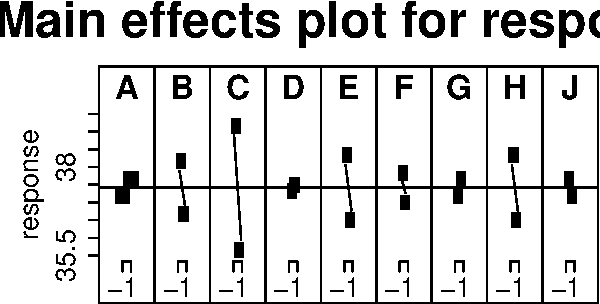
\includegraphics{sciguide_files/figure-latex/pba-1}

\begin{Shaded}
\begin{Highlighting}[]
\KeywordTok{summary}\NormalTok{(}\KeywordTok{lm}\NormalTok{(plan.resp))}
\end{Highlighting}
\end{Shaded}

\begin{verbatim}
## Number of observations used: 12 
## Formula:
## response ~ A + B + C + D + E + F + G + H + J
## 
## Call:
## lm.default(formula = fo, data = model.frame(fo, data = formula))
## 
## Residuals:
##      1      2      3      4      5      6      7      8 
##  1.167  1.333 -1.167  1.333 -1.333 -1.167  1.333 -1.333 
##      9     10     11     12 
##  1.167 -1.333  1.167 -1.167 
## 
## Coefficients:
##             Estimate Std. Error t value Pr(>|t|)    
## (Intercept) 37.41667    0.88585  42.238  0.00056 ***
## A1          -0.08333    0.88585  -0.094  0.93363    
## B1           0.25000    0.88585   0.282  0.80430    
## C1          -0.08333    0.88585  -0.094  0.93363    
## D1           0.25000    0.88585   0.282  0.80430    
## E1          -0.58333    0.88585  -0.659  0.57788    
## F1          -0.08333    0.88585  -0.094  0.93363    
## G1          -1.41667    0.88585  -1.599  0.25089    
## H1          -0.08333    0.88585  -0.094  0.93363    
## J1           1.58333    0.88585   1.787  0.21579    
## ---
## Signif. codes:  
## 0 '***' 0.001 '**' 0.01 '*' 0.05 '.' 0.1 ' ' 1
## 
## Residual standard error: 3.069 on 2 degrees of freedom
## Multiple R-squared:  0.7614,	Adjusted R-squared:  -0.3126 
## F-statistic: 0.7089 on 9 and 2 DF,  p-value: 0.7068
\end{verbatim}

在这里PB设计实际上是一种预选法,如果结果显示某些变量影响显著,那么事实上就可以针对这些变量进行进一步的精细筛选,其余的变量可以直接固定为一个水平进行进一步设计。PB法在工业届用的比较多,但你应该想到了,如果只是进行变量选择,为啥不用随机森林或lasso?其实都可以,但这些方法不是设计而更多是数据分析通用方法,设计上除了最重要的随机性也是要考虑各因子贡献或者说重复数尽量平衡些的,否则会过分偏重某个因子,或者干脆配对或组成区组。像这样不做预设去设计对各个因子都公平,如果有预设或现实条件不允许,也可以裂区设计。

当选出重要因素时,下一步常见是正交试验或响应面分析,用来优选参数。正交表这玩意我在书中没找到,文献里用得多的也是亚洲人,老外统一用析因试验来进行考察。其实正交表的设计原理就是用尽量少的步骤遍历掉因子空间,这样进行一定次数试验就可以发现最优组合。R中的实现基本都在\texttt{DoE.base} 包里,这个包内置了一堆可以直接调用的正交表,可以根据需求进行查询。例如我有6个因素,水平数分别是2,3,3,2,2,6,然后我只打算做不超过54次试验,这时可以直接调用\texttt{show.oas}函数进行查询,给出的正交表随意选一个就可以继续。

\begin{Shaded}
\begin{Highlighting}[]
\KeywordTok{show.oas}\NormalTok{(}\DataTypeTok{nruns =} \KeywordTok{c}\NormalTok{(}\DecValTok{0}\NormalTok{, }\DecValTok{54}\NormalTok{), }\DataTypeTok{nlevels =} \KeywordTok{c}\NormalTok{(}\DecValTok{2}\NormalTok{, }\DecValTok{3}\NormalTok{, }\DecValTok{3}\NormalTok{, }\DecValTok{2}\NormalTok{, }\DecValTok{2}\NormalTok{, }\DecValTok{6}\NormalTok{), }\DataTypeTok{showmetrics =} \OtherTok{TRUE}\NormalTok{)}
\end{Highlighting}
\end{Shaded}

\begin{verbatim}
## no suitable  resolution IV or more  array found
## 5  orthogonal  arrays found
##                name nruns lineage   GR GRind regular SCones
## 78 L36.2.13.3.2.6.1    36         3.00  3.00   FALSE      6
## 81 L36.2.10.3.8.6.1    36         3.18  3.18   FALSE      0
## 83  L36.2.9.3.4.6.2    36         3.00  3.00   FALSE     17
## 87  L36.2.3.3.9.6.1    36         3.18  3.00   FALSE     12
## 88  L36.2.3.3.2.6.3    36         3.00  3.00   FALSE     37
##       A3    A4   A5    A6      A7      A8
## 78  45.3 158.4  426  1010  1753.2  2306.8
## 81 130.3 737.2 3063 11096 31380.8 68828.1
## 83  82.3 338.2 1025  2828  5507.5  7780.0
## 87  73.8 300.2  912  2404  4354.2  5793.4
## 88  35.6  73.1  120   125    63.5    13.9
\end{verbatim}

这里我们选分辨率略高的\texttt{L36.2.10.3.8.6.1},从名字上看,这是一个36次试验表,可以包含10个两水平,8个三水平与1个六水平因子,这也是唯一一个分辨率高于3,可以排除交互作用的设计方法。这里我反复提到分辨率,实际上就是一种考察试验设计合理性的指标,分辨率3一般指只能区分没有交互作用的各因子贡献差异,高于3就可以区分一定的因子交互作用,可以用\texttt{GR}去计算一个广义分辨率并用\texttt{oa.design}来进一步优化这个设计,因为其实符合正交表只是众多选择的一个子集,不过根据优化方法的不同,优化时间也不太一样。

\begin{Shaded}
\begin{Highlighting}[]
\KeywordTok{oa.design}\NormalTok{(L36.}\DecValTok{2}\NormalTok{.}\DecValTok{10}\NormalTok{.}\DecValTok{3}\NormalTok{.}\DecValTok{8}\NormalTok{.}\FloatTok{6.1}\NormalTok{, }\DataTypeTok{nlevels =} \KeywordTok{c}\NormalTok{(}\DecValTok{2}\NormalTok{, }\DecValTok{3}\NormalTok{, }\DecValTok{3}\NormalTok{, }\DecValTok{2}\NormalTok{, }\DecValTok{2}\NormalTok{, }\DecValTok{6}\NormalTok{), }\DataTypeTok{columns =} \StringTok{"min34"}\NormalTok{)}
\end{Highlighting}
\end{Shaded}

\begin{verbatim}
##    A B C D E F
## 1  1 1 3 2 1 4
## 2  2 2 1 2 2 3
## 3  1 2 3 1 1 1
## 4  2 2 1 2 1 5
## 5  1 1 1 1 1 1
## 6  2 1 1 2 1 2
## 7  1 2 2 2 2 2
## 8  2 3 3 1 2 3
## 9  1 3 1 1 1 3
## 10 1 2 1 1 2 4
## 11 1 3 2 2 1 2
## 12 2 1 2 1 2 4
## 13 2 3 1 1 1 4
## 14 1 1 2 2 2 3
## 15 1 2 2 1 1 3
## 16 2 1 3 2 2 1
## 17 1 2 3 2 2 5
## 18 1 1 3 1 2 2
## 19 1 3 2 1 2 6
## 20 1 1 2 1 1 5
## 21 2 1 1 1 2 5
## 22 2 3 2 2 1 1
## 23 2 3 2 2 2 5
## 24 2 2 2 1 2 1
## 25 2 1 2 1 1 6
## 26 2 2 2 2 1 4
## 27 1 1 1 2 2 6
## 28 2 3 3 2 1 6
## 29 2 2 3 1 1 2
## 30 2 2 3 1 2 6
## 31 1 3 3 1 1 5
## 32 2 1 3 2 1 3
## 33 2 3 1 1 2 2
## 34 1 3 1 2 2 1
## 35 1 3 3 2 2 4
## 36 1 2 1 2 1 6
## class=design, type= oa
\end{verbatim}

使用这个函数你就不用费力去套正交表了,直接可以用输出的设计方案,记得要说明你的分辨率优化方案。如果你坚持套正交表,一定要理解如何去套,因为正交表的排列是很讲究的,特别是你要考虑交互作用的影响。如果一个表最多14个因子而你就设计了14个因子,那么分辨率不会超过3。正交设计的分析与前面PB设计是一致的,都是沿用添加响应,然后方差分析或线性分析随意来就是了,\texttt{DoE.base} 包为\texttt{design}这个对象类型设置了\texttt{lm}与\texttt{aov}方法。

在进行数据分析时,有时会遇到方差分析与线性回归的区别问题,打比方你用线性回归来做分析,会有审稿人问你lack of fit检验有没有做。这个检验实质上也是个F检验,用来衡量线性模型之外残差里分组变异与纯误差变异的比值,如果分组变异还是比较大,那么线性假设可能就不合理。

不过,目前试验设计结果分析更精细的会用响应面分析。顾名思义,响应面有点梯度下降迭代寻优的意思,而且如果是曲面通常考虑了二阶甚至更高阶的交互作用。在R中的实现是通过 \texttt{rsm} 包来进行的,这个包也是囊括了设计与分析两个部分,设计部分也有常见的 Box-Wilson Central Composite Designs 与Box-Behnken designs,分析部分自然还是基于\texttt{lm}的。同样,对于CCD设计,也提供了\texttt{ccd.pick}来选择好的设计,这里好自然意味着一些表征设计均衡的统计量。因为\texttt{rsm} 包小品文写的很清楚了,我就略过演示了。如果你面临多响应同步优化问题,那么\texttt{desirability}包考虑一下有没有,这个包其实是定义了一个多响应的联合满意度作为目标统计量,然后用响应面分析进行寻优,对于组学研究是有启发的。另外说个小八卦,狭义正交表也就是田口设计其实最初是两响应优化,只不过另一个响应是无法控制的噪音,田口搞了个信噪比来解决问题,熟悉了这套统计量构建策略,你也应该能做到根据实际情况构建指标体系。

其实试验设计分析是可以用所有符合\(y = f(x)\)的模型来操作的,说白了就是参数寻优。但试验设计更独特的点就在设计上,更广义地讲,A/B测试等纯计算试验也可以套用试验设计原理,这里要区分清楚设计与分析,设计不合理,分析会很头痛。如果再扩展些,观察研究的试验设计相比控制实验更关注配对或策略抽样。总之试验设计并不是什么水晶球,其原则从来都很清楚,只是后来流派出的太多,术语也越来越晦涩。然后你就会在网上看到哪个软件能做哪个分析的讨论了,其实这情况在工科可能更严重些,例如混料配比的\href{https://support.minitab.com/zh-cn/minitab/18/help-and-how-to/modeling-statistics/doe/supporting-topics/mixture-designs/what-is-a-mixture-design/}{三角坐标系设计}就完全是另一套,不过万变不离其宗,说白了还是个响应面分析。

\hypertarget{ux5b9aux6027ux5b9eux9a8c}{%
\section{定性实验}\label{ux5b9aux6027ux5b9eux9a8c}}

\hypertarget{ux4fe1ux5ea6ux6548ux5ea6}{%
\subsection{信度效度}\label{ux4fe1ux5ea6ux6548ux5ea6}}

\hypertarget{ux5747ux8d28ux5f02ux8d28ux6027}{%
\subsection{均质异质性}\label{ux5747ux8d28ux5f02ux8d28ux6027}}

\hypertarget{ux5b9aux91cfux5b9eux9a8c}{%
\section{定量实验}\label{ux5b9aux91cfux5b9eux9a8c}}

\hypertarget{ux57faux7ebf}{%
\subsection{基线}\label{ux57faux7ebf}}

祖母的身高缩水、罗马俱乐部与基线不明,营养改善现状

\hypertarget{ux6307ux6807ux5316}{%
\subsection{指标化}\label{ux6307ux6807ux5316}}

现代人的物质与能量需求核算 单人一年十平概念下需要多少生存成本 用巨无霸指数换算

汉堡王老干妈与指标

\hypertarget{ux9884ux5b9eux9a8c}{%
\section{预实验}\label{ux9884ux5b9eux9a8c}}

\hypertarget{ux601dux60f3ux5b9eux9a8c}{%
\section{思想实验}\label{ux601dux60f3ux5b9eux9a8c}}

\begin{itemize}
\tightlist
\item
  \href{https://www.vox.com/technology/2016/6/23/12007694/elon-musk-simulation-cartoon}{人是否在仿真中}
\end{itemize}

\hypertarget{data}{%
\chapter{数据处理}\label{data}}

数据处理是科研中很重要的一环,同样的数据不同的人处理会得到不同的结论。事实只有一个,但解释可以有很多,数据处理方式本身就会对解释产生影响。这里重点讨论几个常见的数据处理问题。

\hypertarget{ux63a2ux7d22ux6027ux6570ux636eux5206ux6790ux4e0eux53efux89c6ux5316}{%
\section{探索性数据分析与可视化}\label{ux63a2ux7d22ux6027ux6570ux636eux5206ux6790ux4e0eux53efux89c6ux5316}}

\hypertarget{ux591aux91cdux6bd4ux8f83}{%
\section{多重比较}\label{ux591aux91cdux6bd4ux8f83}}

方差分析解决的是分类变量对响应变量的影响问题,通常是用分类变量所解释的变异比上分类变量以外的变异去进行F检验。换句话讲,如果分类变量可以解释大部分响应变量的变异,我们就说这种分类变量对响应变量的解释有意义。例如下面这组数据:

\begin{quote}
1, 1, 1, 1, 1, 2, 2, 2, 2, 2, 3, 3, 3, 3, 3
\end{quote}

总变异为10, 如果我们分组为按照相同的数放到一起,那么组内变异就是0,组间变异为10,这时我们就说这种分组有效的解释了响应变量,F值趋向正无穷。如果我们完全随机分组,组内与组间的变异差不多,那么这种分类方法并不解释响应变量,反映到F值上就是1。

但是仅仅知道是否受影响是不够的,如同上面的例子,我们知道的仅仅是存在一种分类方法可以解释响应的全部变化,其内部也是均匀的,但不同分类水平间的差异我们并不知道,这就是多重比较的起源。实际生活中如果差异很明显往往统计学工具不用出场,所以你应该预想到多重比较或仅仅是均值比较适用的场景往往差异我们不能直观感受,需要统计学工具来帮忙。

同时要注意,如果我们对两组数据做置信度0.05的t检验,我们遇到假阳性的概率为5\%。但如果面对多组数据例如3组,进行两两比较的话就有\[choose(3,2)\]也就是3组对比,那么我们遇到假阳性的概率就为\[1-(1-0.05)^3\],也就是14.3\%,远高于0.05的置信度。组越多,两两对比就越多,整体上假阳性的概率就越来越大,到最后就是两组数据去对比,无论如何你都会检验出差异。

那么多重比较如何应对这个问题呢?有两种思路,一种思路是我依旧采取两两对比,进行t检验,但p值的选取方法要修改,例如Bonferroni方法中就把p的阈值调整为进行多重比较的次数乘以计算得到的p值。如果我们关心的因素为2,那么计算得到的p值都要乘2来跟0.05或0.01的边界置信度进行比较;另一种思路则是修改两两比较所用的统计量,给出一个更保守的分布,那么得到p值就会更大。不论怎样,我们这样做都是为了降低假阳性,但同时功效不可避免的降低了。

我们设计一个实验考察一个因素对响应变量的影响,结论无过于有影响,没影响。多重比较的前提是有影响,给出的答案是对影响的估计:影响有多大。那我们重复这个实验所要考虑的问题就是能否重现影响,影响的方向与大小是否与文献报道一致。

就方向而样,虽然我们都不承认0假设(要不然还做什么实验),但当我们默认设定为双尾检验时,假阳性就被默认发生在两个方向上了,这样的多重比较必然导致在其中一个方向上的错误率被夸大了。

就影响大小而言,如果我们每次重复都选择效应最强的那一组,重复越多,预设的偏态就越重,换言之,我们的零假设因为重复实验的选择偏好而发生了改变。

这是多重比较里常见的错误类型:

\begin{itemize}
\tightlist
\item
  type I 假阳性

  \begin{itemize}
  \tightlist
  \item
    per-comparison error rate (PCER) 进行多次对比得到的假阳性的概率
  \item
    familywise error rate (FWER) 将多组比较看作一个大组,这时造成的错误率
  \item
    false discovery rate (FDR) 控制假阳性与总拒绝率的比例
  \item
    一般而言 PCER ≤ FDR ≤ FWER FWER更容易不拒绝空假设,更保守
  \end{itemize}
\item
  type II 假阴性
\item
  type III 有差异 方向错误
\end{itemize}

多重比较的方法类型

\begin{itemize}
\tightlist
\item
  Single-step procedures 单步法 只考虑对H0的影响,不考虑其他影响
\item
  Stepwise procedures 逐步法 考虑其他假设检验对单一检验的影响

  \begin{itemize}
  \tightlist
  \item
    Step-down procedures 排序后先对比第一个,有差异对比下一个,当出现无差异时停止对比
  \item
    Step-up procedures 排序后对比,有差异时停止对比,之后均认为有差异
  \end{itemize}
\item
  两两比较 不同组之间进行均值比较,最常见
\item
  对比 除了考虑不同组间均值比较,还考虑均值间线性组合的新均值的差异性,F检验有时是因为对比而不是两两比较产生的显著性
\end{itemize}

\hypertarget{ux5355ux6b65ux6cd5ux7b49ux65b9ux5dee}{%
\subsection{单步法等方差}\label{ux5355ux6b65ux6cd5ux7b49ux65b9ux5dee}}

\emph{Tukey's HSD(两两比较)}

\begin{itemize}
\tightlist
\item
  基于t范围分布
\item
  等方差同数目,如果数目不同则使用Tukey-Kranmer方法
\item
  两两比较最佳,数目相同功效弱于下降法
\end{itemize}

\emph{Bonferroni(两两比较)}

\begin{itemize}
\tightlist
\item
  切割α,如果进行了c次推断,整个错误率为cα
\item
  通用方法,应用在任一个推断
\item
  方法简单,但十分保守
\item
  只对比部分的话可自定义c值
\item
  适用于指定对比数情况,此时功效高于Tukey
\end{itemize}

\emph{DST(两两比较)}

\begin{itemize}
\tightlist
\item
  对Boneferroni方法的改进,功效更高
\end{itemize}

\emph{GT2 test(两两比较)}

\begin{itemize}
\tightlist
\item
  功效高于Dunn-Sidak方法
\end{itemize}

\emph{Gabriel(两两比较)}

\begin{itemize}
\tightlist
\item
  分组数目相同等同于GT2,不同时功效高,但不保证α
\item
  易于可视化
\end{itemize}

\emph{Scheffe test(两两比较)}

\begin{itemize}
\tightlist
\item
  两两比较中功效最弱
\end{itemize}

\emph{Tukey's HSD(对比)}

\begin{itemize}
\tightlist
\item
  涉及2~3个均值时功效最高
\end{itemize}

\emph{Bonferroni(对比)}

\begin{itemize}
\tightlist
\item
  指定对比数
\end{itemize}

\emph{DST(对比)}

\begin{itemize}
\tightlist
\item
  指定对比数,功效高于Bonferroni
\end{itemize}

\emph{Scheffe test(对比)}

\begin{itemize}
\tightlist
\item
  保证α,两两比较功效最高
\end{itemize}

\hypertarget{ux5355ux6b65ux6cd5ux5f02ux65b9ux5deeux5bf9ux6bd4ux4e0eux4e24ux4e24ux6bd4ux8f83}{%
\subsection{单步法异方差(对比与两两比较)}\label{ux5355ux6b65ux6cd5ux5f02ux65b9ux5deeux5bf9ux6bd4ux4e0eux4e24ux4e24ux6bd4ux8f83}}

\emph{GH procedure}

\begin{itemize}
\tightlist
\item
  不保证整体错误率,有时会超过,保守但功效高
\end{itemize}

\emph{C}

\begin{itemize}
\tightlist
\item
  保证整体错误率
\end{itemize}

\emph{T3}

\begin{itemize}
\tightlist
\item
  保证整体错误率
\end{itemize}

Brown-Forsythe-Scheffe

\begin{itemize}
\tightlist
\item
  功效最高
\end{itemize}

\hypertarget{ux5355ux6b65ux6cd5ux7a7aux767dux5bf9ux6bd4}{%
\subsection{单步法空白对比}\label{ux5355ux6b65ux6cd5ux7a7aux767dux5bf9ux6bd4}}

\emph{Dunnett}

\begin{itemize}
\tightlist
\item
  用于对比controls的变化
\item
  其他组对比不考虑
\end{itemize}

\emph{Hsu's MCB}

\begin{itemize}
\tightlist
\item
  对比均值与其他最好(自定义,可最大,亦可最小)
\item
  目的寻找比其他好的而不是不同的
\item
  对比次数最少,功效强,但低于Dunnett
\end{itemize}

\hypertarget{stepdown-procedures}{%
\subsection{Stepdown procedures}\label{stepdown-procedures}}

\begin{itemize}
\tightlist
\item
  基于Tukey法
\item
  先比较最大最小,q值取分组数
\item
  比较最大第二小,q取分组数-1
\item
  继续直到出现无差异停止
\item
  当不需要置信区间且样本数相同时使用
\item
  不推荐SNK与Duncan,推荐REGWF或REGWQ方法
\end{itemize}

\emph{SNK}

\begin{itemize}
\tightlist
\item
  不保证α
\end{itemize}

\emph{Duncan}

\begin{itemize}
\tightlist
\item
  不保证α
\end{itemize}

\emph{Ryan-Einot-Gabriel-Welsch-Fisher(REGWF)}

\begin{itemize}
\tightlist
\item
  F检验加强版,保证α
\end{itemize}

\emph{Ryan-Einot-Gabriel-Welsch-Q(REGWQ)}

\begin{itemize}
\tightlist
\item
  q值法加强版,保证α
\end{itemize}

\hypertarget{step-up-procedures}{%
\subsection{step-up procedures}\label{step-up-procedures}}

\begin{itemize}
\tightlist
\item
  Welsch
\item
  Hochberg
\item
  Dunnett and Tamhane
\end{itemize}

\hypertarget{ux591aux91cdux6bd4ux8f83ux7b80ux7565ux9009ux62e9ux6307ux5357}{%
\subsection{多重比较简略选择指南}\label{ux591aux91cdux6bd4ux8f83ux7b80ux7565ux9009ux62e9ux6307ux5357}}

\emph{总体控制错误率}

\begin{itemize}
\tightlist
\item
  两两比较用Tukey法
\item
  对比用Scheffe test
\item
  指定对比数考虑 Gabriel \textgreater{} GT2 \textgreater{} DST \textgreater{} Bonferroni
\item
  跟control比较用Dunnett
\item
  方差不相等用GH,C,T3等方法
\end{itemize}

\emph{错误率}

\begin{itemize}
\tightlist
\item
  保证α用Tukey Scheffe Dunnett
\item
  不保证用其他的
\end{itemize}

\emph{探索与确认}

\begin{itemize}
\tightlist
\item
  事前分析确定对比数用 Gabriel GT2或Scheffe
\item
  事后确定对比用Tukey或各种stepwise方法
\end{itemize}

\hypertarget{ux53c2ux8003ux8d44ux6599}{%
\subsection{参考资料}\label{ux53c2ux8003ux8d44ux6599}}

\begin{itemize}
\tightlist
\item
  Rafter, J.A., Abell, M.L., Braselton, J.P., 2002. Multiple comparison methods for means. Siam Review 44, 259--278.
\item
  \url{http://cos.name/cn/topic/142002}
\item
  多重比较问题 \url{https://www.nature.com/articles/nbt1209-1135}
\item
  Bretz, F., Hothorn, T., Westfall, P., 2010. Multiple Comparisons Using R. CRC Press.
  Gabriel, K.R., 1978. A Simple Method of Multiple Comparisons of Means. J. Am. Stat. Assoc. 73, 724. \url{https://doi.org/10.2307/2286265}
\item
  Gelman, A., Hill, J., Yajima, M., 2009. Why we (usually) don't have to worry about multiple comparisons. ArXiv09072478 Stat.
\item
  Plotting of multiple comparisons? {[}WWW Document{]}, n.d. URL \url{http://stackoverflow.com/questions/2286085/plotting-of-multiple-comparisons} (accessed 11.9.13).
\item
  Rafter, J.A., Abell, M.L., Braselton, J.P., 2002. Multiple comparison methods for means. Siam Rev.~44, 259--278.
  Stoline, M.R., Ury, H.K., 1979. Tables of the Studentized Maximum Modulus Distribution and an Application to Multiple Comparisons among Means. Technometrics 21, 87. \url{https://doi.org/10.2307/1268584}
\item
  \href{https://zh.wikipedia.org/wiki/\%E5\%A4\%9A\%E9\%87\%8D\%E6\%AF\%94\%E8\%BC\%83\%E8\%AC\%AC\%E8\%AA\%A4}{多重比较谬误}
\end{itemize}

\hypertarget{ux591aux91cdux68c0ux9a8c}{%
\section{多重检验}\label{ux591aux91cdux68c0ux9a8c}}

各种组学分析技术的进展导致了我们在收集数据时更侧重数据信息的保存,然而我们收集的数据最终也会根据我们的想探索的问题来寻找答案,甚至有时候我们在实验设计分组时就打算考察某一个变量而为了获取更多的相关信息而采用了组学技术。这点是尤其要强调的,科研人员一定是面向科学问题解决科学问题,而不要为了应用新技术而应用新技术。当然,现实的情况是新技术特别是组学技术的发展为我们提供了大量的可同时测定的生物学指标(例如基因表达水平、蛋白表达水平、代谢产物表达水平)数据,大到我们事先也不知道会有什么模式会出现,这样就需要数据挖掘,特别是统计学知识来帮助我们发现新知。然而,组学技术产生的这类高通量数据是具有一些特质的,数据里确实会有我们关心分组的差异表达,但同时也有大量测量值对于我们设定的分组不敏感,然而当我们去对比组间差异时就会被这些数据干扰。

举例而言,我对两组样品(暴露组跟对照组)中每一个样品测定了10000个指标,每组有10个样品,那么如果我想知道差异有多大就需要对比10000次,具体说就是10000次双样本t检验。那么如果我对t检验的置信水平设置在0.05,也就是5\%假阳性,做完这10000次检验,我会期望看到500个假阳性,而这500个有显著差异的指标其实对分组不敏感也可以随机生成。假如真实测到了600个有显著差异的指标,那么如何区分其中哪些是对分组敏感?哪些又仅仅只是随机的呢?随机的会不会只有500个整呢?

这就是多重检验问题,做经典科研实验时往往会忽略,深层次的原因是经典的科研实验往往是理论或经验主导需要进行检验的假说。例如,我测定血液中白血球的数目就可以知道你是不是处于炎症中,其背后是医学知识的支撑。然而,再组学或其他高通量实验中,研究实际是数据导向的,也就是不管有用没用反正我测了一堆指标,然后就去对比差异,然后就是上面的问题了,我们可能分不清楚哪些是真的相关,哪些又是随机出现的。

当然这个问题出现也不是一天两天了,在\href{http://yufree.cn/blogcn/2013/12/16/rgabriel-package.html}{多重比较}问题上就已经被提出过,只不过在多重比较里对比数因为排列组合比较多而在多重检验里纯粹就是因为同时进行的假设检验数目多。那么其实从统计角度解决的方法也基本来源于此。

对于单次比较,当我们看到显著差异的p值脑子里想的是空假设为真时发生的概率,当我们置信水平设定在0.95(I型错误率0.05)而p值低于对应的阈值,那么我们应该拒绝空假设。但对比次数多了从概率上就会出现已经被拒绝的假设实际是错误的而你不知道是哪一个。整体错误率控制的思路就是我不管单次比较了,我只对你这所有的对比次数的总错误率进行控制。还是上面的例子,对于10000次假设检验我只能接受1个错误,整体犯错概率为0.0001,那么对于单次比较,其I型错误率也得设定在这个水平上去进行假设检验,结果整体上错误率是控制住了,但对于单次比较就显得十分严格了。下面用一个仿真实验来说明:

\begin{Shaded}
\begin{Highlighting}[]
\CommentTok{# 随机数的10000次比较}
\KeywordTok{set.seed}\NormalTok{(}\DecValTok{42}\NormalTok{)}
\NormalTok{pvalue <-}\StringTok{ }\OtherTok{NULL}
\ControlFlowTok{for}\NormalTok{ (i }\ControlFlowTok{in} \DecValTok{1}\OperatorTok{:}\DecValTok{10000}\NormalTok{) \{}
\NormalTok{    a <-}\StringTok{ }\KeywordTok{rnorm}\NormalTok{(}\DecValTok{10}\NormalTok{)}
\NormalTok{    b <-}\StringTok{ }\KeywordTok{rnorm}\NormalTok{(}\DecValTok{10}\NormalTok{)}
\NormalTok{    c <-}\StringTok{ }\KeywordTok{t.test}\NormalTok{(a, b)}
\NormalTok{    pvalue[i] <-}\StringTok{ }\NormalTok{c}\OperatorTok{$}\NormalTok{p.value}
\NormalTok{\}}
\CommentTok{# 看下p值分布}
\KeywordTok{hist}\NormalTok{(pvalue)}
\end{Highlighting}
\end{Shaded}

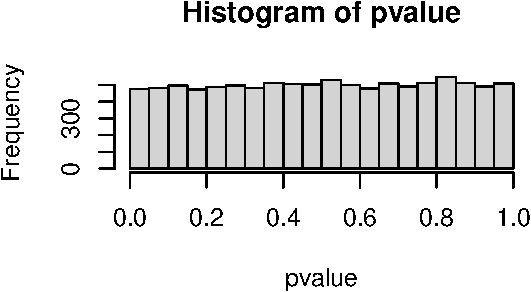
\includegraphics{sciguide_files/figure-latex/unnamed-chunk-5-1}

\begin{Shaded}
\begin{Highlighting}[]
\CommentTok{# 小于0.05的个数}
\KeywordTok{sum}\NormalTok{(pvalue }\OperatorTok{<}\StringTok{ }\FloatTok{0.05}\NormalTok{)}
\end{Highlighting}
\end{Shaded}

\begin{verbatim}
## [1] 477
\end{verbatim}

\begin{Shaded}
\begin{Highlighting}[]
\CommentTok{# 小于0.0001的个数}
\KeywordTok{sum}\NormalTok{(pvalue }\OperatorTok{<}\StringTok{ }\FloatTok{1e-04}\NormalTok{)}
\end{Highlighting}
\end{Shaded}

\begin{verbatim}
## [1] 0
\end{verbatim}

这样我们会看到进行了整体的控制之后,确实是找不到有差异的了,但假如里面本来就有有差异的呢?

\begin{Shaded}
\begin{Highlighting}[]
\KeywordTok{set.seed}\NormalTok{(}\DecValTok{42}\NormalTok{)}
\NormalTok{pvalue <-}\StringTok{ }\OtherTok{NULL}
\ControlFlowTok{for}\NormalTok{ (i }\ControlFlowTok{in} \DecValTok{1}\OperatorTok{:}\DecValTok{10000}\NormalTok{) \{}
\NormalTok{    a <-}\StringTok{ }\KeywordTok{rnorm}\NormalTok{(}\DecValTok{10}\NormalTok{, }\DecValTok{1}\NormalTok{)}
\NormalTok{    b <-}\StringTok{ }\NormalTok{a }\OperatorTok{+}\StringTok{ }\DecValTok{1}
\NormalTok{    c <-}\StringTok{ }\KeywordTok{t.test}\NormalTok{(a, b)}
\NormalTok{    pvalue[i] <-}\StringTok{ }\NormalTok{c}\OperatorTok{$}\NormalTok{p.value}
\NormalTok{\}}
\CommentTok{# 看下p值分布}
\KeywordTok{hist}\NormalTok{(pvalue)}
\end{Highlighting}
\end{Shaded}

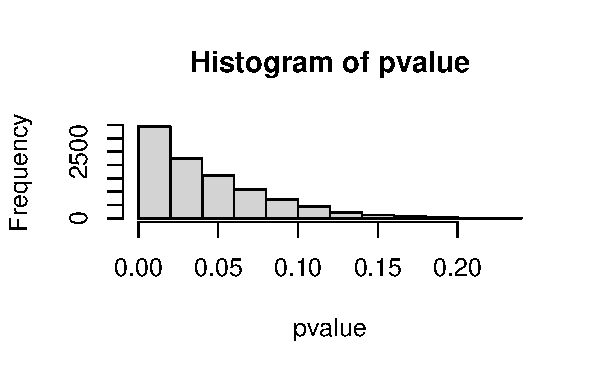
\includegraphics{sciguide_files/figure-latex/unnamed-chunk-6-1}

\begin{Shaded}
\begin{Highlighting}[]
\CommentTok{# 小于0.05的个数}
\KeywordTok{sum}\NormalTok{(pvalue }\OperatorTok{<}\StringTok{ }\FloatTok{0.05}\NormalTok{)}
\end{Highlighting}
\end{Shaded}

\begin{verbatim}
## [1] 6559
\end{verbatim}

\begin{Shaded}
\begin{Highlighting}[]
\CommentTok{# 小于0.0001的个数}
\KeywordTok{sum}\NormalTok{(pvalue }\OperatorTok{<}\StringTok{ }\FloatTok{1e-04}\NormalTok{)}
\end{Highlighting}
\end{Shaded}

\begin{verbatim}
## [1] 45
\end{verbatim}

上面我们模拟了10000次有真实差异的假设检验,结果按照单次检验0.05的阈值能发现约7000有差异,而使用0.0001却只能发现不到100次有显著差异。那么问题很明显,或许控制整体错误率可以让我们远离假阳性,但假阴性也就是II型错误率就大幅提高了,最后的结果可能是什么差异也看不到。

下面我们尝试一个更实际的模拟,混合有差异跟无差异的检验:

\begin{Shaded}
\begin{Highlighting}[]
\KeywordTok{set.seed}\NormalTok{(}\DecValTok{42}\NormalTok{)}
\NormalTok{pvalue <-}\StringTok{ }\OtherTok{NULL}
\ControlFlowTok{for}\NormalTok{ (i }\ControlFlowTok{in} \DecValTok{1}\OperatorTok{:}\DecValTok{5000}\NormalTok{) \{}
\NormalTok{    a <-}\StringTok{ }\KeywordTok{rnorm}\NormalTok{(}\DecValTok{10}\NormalTok{, }\DecValTok{1}\NormalTok{)}
\NormalTok{    b <-}\StringTok{ }\NormalTok{a }\OperatorTok{+}\StringTok{ }\DecValTok{1}
\NormalTok{    c <-}\StringTok{ }\KeywordTok{t.test}\NormalTok{(a, b)}
\NormalTok{    pvalue[i] <-}\StringTok{ }\NormalTok{c}\OperatorTok{$}\NormalTok{p.value}
\NormalTok{\}}
\ControlFlowTok{for}\NormalTok{ (i }\ControlFlowTok{in} \DecValTok{1}\OperatorTok{:}\DecValTok{5000}\NormalTok{) \{}
\NormalTok{    a <-}\StringTok{ }\KeywordTok{rnorm}\NormalTok{(}\DecValTok{10}\NormalTok{, }\DecValTok{1}\NormalTok{)}
\NormalTok{    b <-}\StringTok{ }\KeywordTok{rnorm}\NormalTok{(}\DecValTok{10}\NormalTok{, }\DecValTok{1}\NormalTok{)}
\NormalTok{    c <-}\StringTok{ }\KeywordTok{t.test}\NormalTok{(a, b)}
\NormalTok{    pvalue[i }\OperatorTok{+}\StringTok{ }\DecValTok{5000}\NormalTok{] <-}\StringTok{ }\NormalTok{c}\OperatorTok{$}\NormalTok{p.value}
\NormalTok{\}}
\CommentTok{# 看下p值分布}
\KeywordTok{hist}\NormalTok{(pvalue)}
\end{Highlighting}
\end{Shaded}

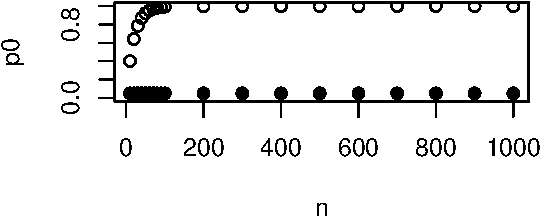
\includegraphics{sciguide_files/figure-latex/unnamed-chunk-7-1}

\begin{Shaded}
\begin{Highlighting}[]
\CommentTok{# 小于0.05的个数}
\KeywordTok{sum}\NormalTok{(pvalue }\OperatorTok{<}\StringTok{ }\FloatTok{0.05}\NormalTok{)}
\end{Highlighting}
\end{Shaded}

\begin{verbatim}
## [1] 3499
\end{verbatim}

\begin{Shaded}
\begin{Highlighting}[]
\CommentTok{# 小于0.0001的个数}
\KeywordTok{sum}\NormalTok{(pvalue }\OperatorTok{<}\StringTok{ }\FloatTok{1e-04}\NormalTok{)}
\end{Highlighting}
\end{Shaded}

\begin{verbatim}
## [1] 21
\end{verbatim}

此时结果就更有意思了,明明应该有5000次是有差异的,但阈值设定在0.05只能看到约3500次,而0.0001只能看到24次。

上面的模拟告诉我们,降低假阳性会提高假阴性的比率,而且似乎本来0.05的阈值对于真阳性也是偏小的。同时,面对假设检验概率低于0.05的那些差异,我们也没有很好的方法区别哪些是真的,哪些是随机的。

其实很多人都知道整体错误率控制是比较严格的,但也不是完全没人用,例如寻找生物标记物做重大疾病诊断时就不太能接受假阳性而可以接受一定的假阴性,此时如果标准放宽就会找到一大堆假信号,到时候标记不准就会对诊断产生负面影响。

下面介绍下常见的两种整体错误率控制方法。

\hypertarget{bonferroni-ux65b9ux6cd5}{%
\subsection{Bonferroni 方法}\label{bonferroni-ux65b9ux6cd5}}

思路很简单,就是控制显著性,例如单次检验假阳性比率\(\alpha\)控制在0.05,那么n次检验假阳性比率控制为\(\frac{\alpha}{n}\)。这样实际是对整体采用了个体控制的控制思路:

\[
P(至少一个显著)=1-P(无显著差异) = 1-(1-\alpha/n)^n
\]

我们来看下\(\alpha = 0.05\)随比较数增加的效果:

\begin{Shaded}
\begin{Highlighting}[]
\NormalTok{n <-}\StringTok{ }\KeywordTok{c}\NormalTok{(}\DecValTok{1}\OperatorTok{:}\DecValTok{10} \OperatorTok\StringTok{ }\DecValTok{10}\OperatorTok{^}\NormalTok{(}\DecValTok{1}\OperatorTok{:}\DecValTok{2}\NormalTok{))}
\NormalTok{p0 <-}\StringTok{ }\DecValTok{1} \OperatorTok{-}\StringTok{ }\NormalTok{(}\DecValTok{1} \OperatorTok{-}\StringTok{ }\FloatTok{0.05}\NormalTok{)}\OperatorTok{^}\NormalTok{n}
\NormalTok{p <-}\StringTok{ }\DecValTok{1} \OperatorTok{-}\StringTok{ }\NormalTok{(}\DecValTok{1} \OperatorTok{-}\StringTok{ }\FloatTok{0.05}\OperatorTok{/}\NormalTok{n)}\OperatorTok{^}\NormalTok{n}
\CommentTok{# 不进行控制}
\KeywordTok{plot}\NormalTok{(p0 }\OperatorTok{~}\StringTok{ }\NormalTok{n, }\DataTypeTok{ylim =} \KeywordTok{c}\NormalTok{(}\DecValTok{0}\NormalTok{, }\DecValTok{1}\NormalTok{))}
\CommentTok{# Bonferroni方法控制}
\KeywordTok{points}\NormalTok{(p }\OperatorTok{~}\StringTok{ }\NormalTok{n, }\DataTypeTok{pch =} \DecValTok{19}\NormalTok{)}
\end{Highlighting}
\end{Shaded}

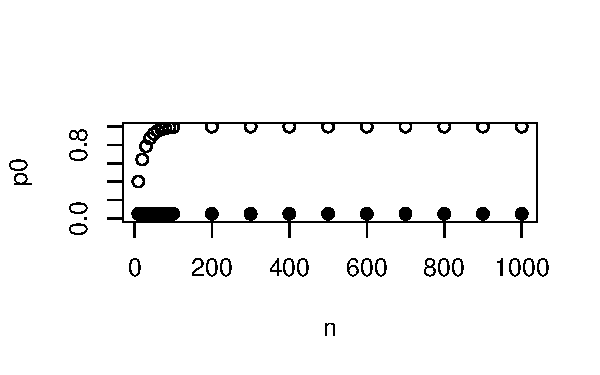
\includegraphics{sciguide_files/figure-latex/unnamed-chunk-8-1}

其实,这样的控制得到的整体错误率是略低于0.05的,并且数目越大,整体错误率越低。这个方法十分保守,有可能什么差异你都看不到,因为都变成假阴性了。在实际应用中一般不调节p值的假阳性比率而直接调节p值,取原始p值跟整体检验数目的乘积与1的最小值作为调节p值,还可以用0.05或0.01进行判断,不过这时候控制的整体而不是单一检验了。

当然这只是最原始的Bonferroni方法,后来Holm改进了这种一步法为逐步法,此时我们需要首先对原始p值进行排序,然后每个原始p值乘上其排序作为调节p值。例如三次多重检验的p值分别是0.01、0.03与0.06,其调节后的p值为0.03,0.06,0.06。如果我们控制整体假阳性比率低于0.05,那么调解后只有第一个检验可以拒绝空假设。值得注意的是Holm的改进是全面优于原始方法的,也就是说当你一定要去用Bonferroni方法控制整体错误率,优先选Holm的改进版。

\hypertarget{sidak-ux65b9ux6cd5}{%
\subsection{Sidak 方法}\label{sidak-ux65b9ux6cd5}}

上面那种方法其实有点非参的意思,其实数学上我们是可以精确的把假阳性比率控制在某个数值的:

\[
P(至少一个显著)=1-P(无显著差异) = 1-(1-\alpha')^n = 0.05
\]

求解可得到\(\alpha' = 1-0.95^{\frac{1}{n}}\),此时我们就可以比较精确的控制整体错误率了,但是,这个方法有个前提就是各个检验必须是独立的,这在生物学实验里几乎不可能,所以这个方法的应用远没有Bonferroni方法广。

\hypertarget{ux9519ux8befux53d1ux73b0ux7387false-discovery-rateux63a7ux5236}{%
\subsection{错误发现率(False Discovery Rate)控制}\label{ux9519ux8befux53d1ux73b0ux7387false-discovery-rateux63a7ux5236}}

刚才的模拟中我们可以看到,控制整体错误率比较严格,假阴性比率高,那么有没有办法找到假阴性比率低的呢?要知道我们其实只关心有差异的那部分中那些是真的,哪些是假的,无差异的可以完全不用考虑。那么我们可以尝试控制错误发现率,也就是在有差异的那一部分指标中控制错误率低于某一水平。

\begin{Shaded}
\begin{Highlighting}[]
\CommentTok{# 所有有差异的}
\NormalTok{R <-}\StringTok{ }\KeywordTok{sum}\NormalTok{(pvalue }\OperatorTok{<}\StringTok{ }\FloatTok{0.05}\NormalTok{)}
\CommentTok{# 假阳性}
\NormalTok{V <-}\StringTok{ }\KeywordTok{sum}\NormalTok{(pvalue[}\DecValTok{5001}\OperatorTok{:}\DecValTok{10000}\NormalTok{] }\OperatorTok{<}\StringTok{ }\FloatTok{0.05}\NormalTok{)}
\CommentTok{# 错误发现率}
\NormalTok{Q <-}\StringTok{ }\NormalTok{V}\OperatorTok{/}\NormalTok{R}
\NormalTok{R}
\end{Highlighting}
\end{Shaded}

\begin{verbatim}
## [1] 3499
\end{verbatim}

\begin{Shaded}
\begin{Highlighting}[]
\NormalTok{V}
\end{Highlighting}
\end{Shaded}

\begin{verbatim}
## [1] 225
\end{verbatim}

\begin{Shaded}
\begin{Highlighting}[]
\NormalTok{Q}
\end{Highlighting}
\end{Shaded}

\begin{verbatim}
## [1] 0.06430409
\end{verbatim}

上面的计算显示虽然我们漏掉了很多阳性结果,但错误发现率并不高。事实上如果我们控制错误率到0.01,错误发现率会更低:

\begin{Shaded}
\begin{Highlighting}[]
\CommentTok{# 所有有差异的}
\NormalTok{R <-}\StringTok{ }\KeywordTok{sum}\NormalTok{(pvalue }\OperatorTok{<}\StringTok{ }\FloatTok{0.01}\NormalTok{)}
\CommentTok{# 假阳性}
\NormalTok{V <-}\StringTok{ }\KeywordTok{sum}\NormalTok{(pvalue[}\DecValTok{5001}\OperatorTok{:}\DecValTok{10000}\NormalTok{] }\OperatorTok{<}\StringTok{ }\FloatTok{0.01}\NormalTok{)}
\CommentTok{# 错误发现率}
\NormalTok{Q <-}\StringTok{ }\NormalTok{V}\OperatorTok{/}\NormalTok{R}
\NormalTok{R}
\end{Highlighting}
\end{Shaded}

\begin{verbatim}
## [1] 999
\end{verbatim}

\begin{Shaded}
\begin{Highlighting}[]
\NormalTok{V}
\end{Highlighting}
\end{Shaded}

\begin{verbatim}
## [1] 34
\end{verbatim}

\begin{Shaded}
\begin{Highlighting}[]
\NormalTok{Q}
\end{Highlighting}
\end{Shaded}

\begin{verbatim}
## [1] 0.03403403
\end{verbatim}

其实出现这个问题不难理解,空假设检验里p值是均匀分布的而有差异检验的p值是有偏分布且偏向于较小的数值,所以假阳性控制的越小,有偏分布占比例就越高,但同时会造成假阴性提高的问题。

那么错误发现率会不会比整体错误率的控制更好呢?这里通过两种常见的控制方法进行说明。

\emph{Benjamini-Hochberg方法}

这个方法跟Holm方法很像,也是先排序,但之后p值并不是简单的乘排序,而是乘检验总数后除排序:

\[
p_i \leq \frac{i}{m} \alpha
\]

举例来说就是假设三次多重检验的p值分别是0.01、0.03与0.06,其调节后的p值为0.03,0.45,0.06。那么为什么说这种方法控制的是错误发现率呢?我们来看下\(\alpha\)是如何得到的:p值乘总数m得到的是在该p值下理论发现数,而除以其排序实际是该p值下实际发现数,理论发现数基于在这里的分布是均匀分布,也就是空假设的分布,这两个的比值自然就是错误发现率。下面我用仿真实验来说明一下:

\begin{Shaded}
\begin{Highlighting}[]
\NormalTok{pbh <-}\StringTok{ }\KeywordTok{p.adjust}\NormalTok{(pvalue, }\DataTypeTok{method =} \StringTok{"BH"}\NormalTok{)}
\NormalTok{ph <-}\StringTok{ }\KeywordTok{p.adjust}\NormalTok{(pvalue, }\DataTypeTok{method =} \StringTok{"holm"}\NormalTok{)}
\KeywordTok{plot}\NormalTok{(pbh }\OperatorTok{~}\StringTok{ }\NormalTok{pvalue)}
\KeywordTok{points}\NormalTok{(ph }\OperatorTok{~}\StringTok{ }\NormalTok{pvalue, }\DataTypeTok{col =} \StringTok{"red"}\NormalTok{)}
\end{Highlighting}
\end{Shaded}

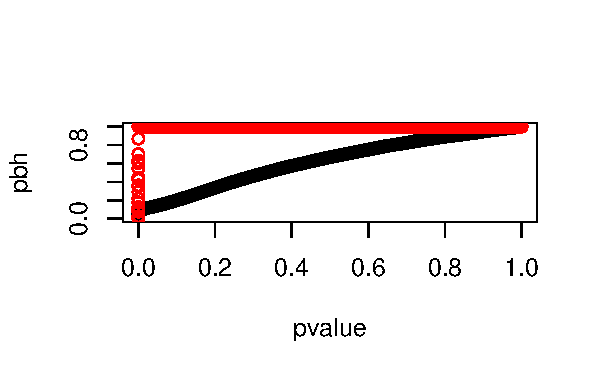
\includegraphics{sciguide_files/figure-latex/unnamed-chunk-11-1}

从上面图我们可以看出,如果控制整体错误率(红色),那么p值很容易就到1了,过于严格。而如果用BH方法控制错误发现率,那么原始p值越大,调节后的错误发现率也逐渐递增,这就符合了区分真实差异与随机差异就要假设真实差异更可能出现更小的p值这个现象。当然至于这个方法的推演细节,可以去读原始论文。值得注意的是这个错误发现率求的是有差异存在的情况,不然零发现就出现除数为零了。

\emph{Storey方法(q值)}

如果说BH方法还算是调节了p值,那么Storey提出的方法则直接去估计了错误发现率本身。刚才介绍BH算法时我提到总数m与p值的乘积是基于这里的分布是均匀分布,但实际上按照错误发现率的定义,这里应该出现的是空假设总数。直接使用所有检验数会造成一个问题,那就是对错误发现率的高估,为了保证功效,这里应该去估计空假设的总体比例。这里我们去观察混合分布会发现在p值较大的时候基本可以认为这里分布的都是空假设的p值,那么我们可以用:

\[
\hat\pi_0 = \frac{\#\{p_i>\lambda\}}{(1-\lambda)m}
\]

估计这个比例\(\hat\pi_0\),其中参数\(\lambda\)的跟\(\hat\pi_0\)的关系可以用一个三阶方程拟合,然后计算出整体假阳性比例。有了这个比例,我们再去按照BH方法计算p值,然后两个相乘就会得到q值,而q值的理论含义就是在某一概率上低于这个概率所有数里假阳性的比重。打个比方,我测到某个指标的q值是0.05,这意味着q值低于这个数所有检验中我有0.05的可能性得到的是假阳性。。但我们会发现当空假设比重较高时BH结果跟q值很接近,而比重很低的话q值会变得更小,功效会提高,基本也符合我们对错误发现率的预期。

\begin{Shaded}
\begin{Highlighting}[]
\KeywordTok{library}\NormalTok{(qvalue)}
\NormalTok{q <-}\StringTok{ }\KeywordTok{qvalue}\NormalTok{(pvalue)}
\CommentTok{# Q值}
\KeywordTok{plot}\NormalTok{(q}\OperatorTok{$}\NormalTok{qvalues }\OperatorTok{~}\StringTok{ }\NormalTok{pvalue, }\DataTypeTok{col =} \StringTok{"blue"}\NormalTok{)}
\end{Highlighting}
\end{Shaded}

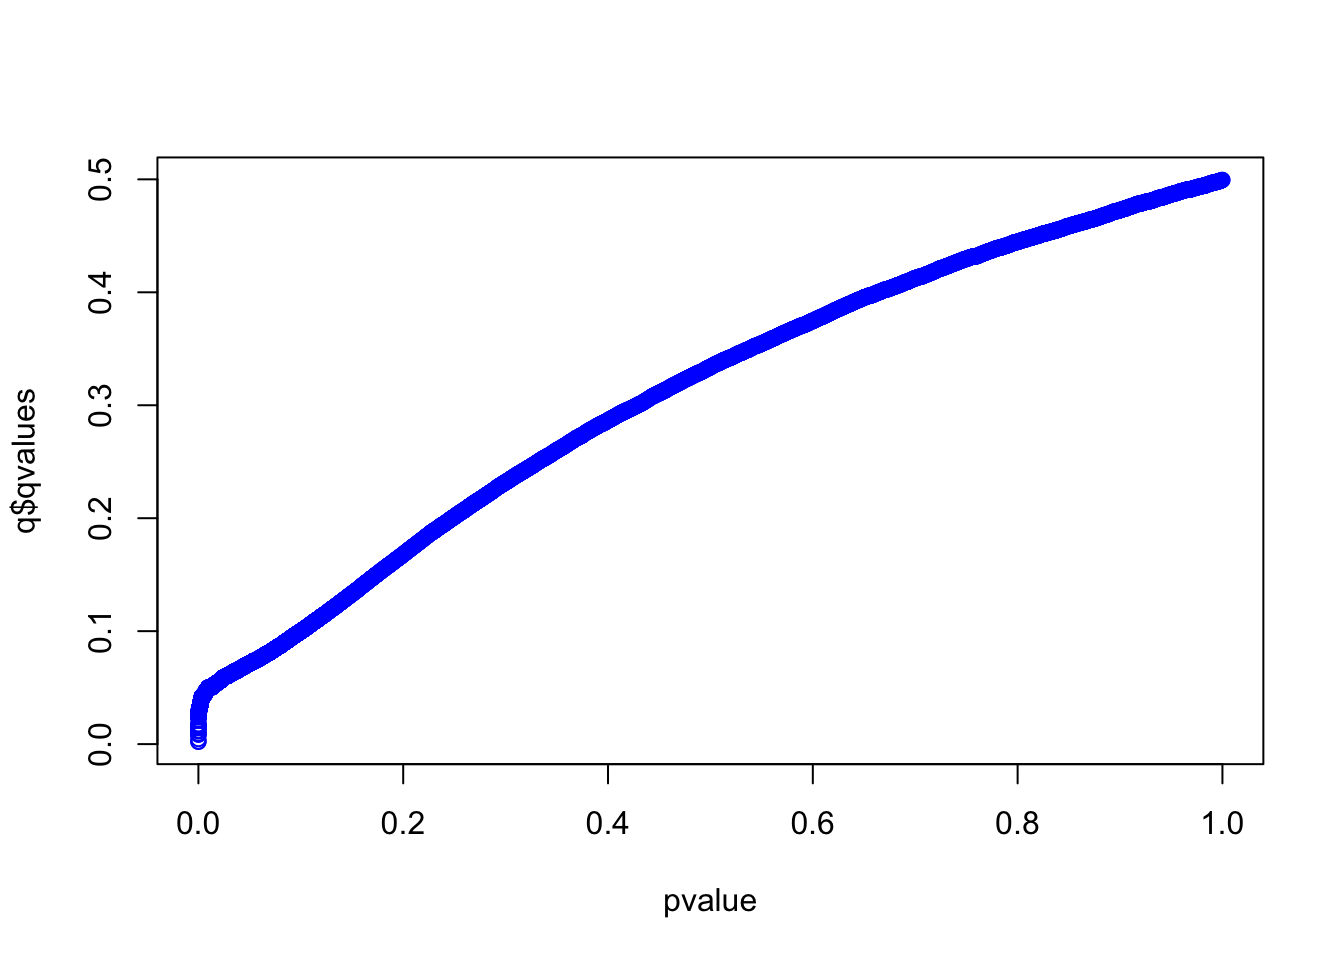
\includegraphics{sciguide_files/figure-latex/unnamed-chunk-12-1}

如上图所示,q值增大后会最终逼近到0.5,而我们的模拟中空假设的比例就设定就是50\%。我们重新模拟一个空假设比例5\%的实验:

\begin{Shaded}
\begin{Highlighting}[]
\KeywordTok{set.seed}\NormalTok{(}\DecValTok{42}\NormalTok{)}
\NormalTok{pvalue <-}\StringTok{ }\OtherTok{NULL}
\ControlFlowTok{for}\NormalTok{ (i }\ControlFlowTok{in} \DecValTok{1}\OperatorTok{:}\DecValTok{500}\NormalTok{) \{}
\NormalTok{    a <-}\StringTok{ }\KeywordTok{rnorm}\NormalTok{(}\DecValTok{10}\NormalTok{, }\DecValTok{1}\NormalTok{)}
\NormalTok{    b <-}\StringTok{ }\NormalTok{a }\OperatorTok{+}\StringTok{ }\DecValTok{1}
\NormalTok{    c <-}\StringTok{ }\KeywordTok{t.test}\NormalTok{(a, b)}
\NormalTok{    pvalue[i] <-}\StringTok{ }\NormalTok{c}\OperatorTok{$}\NormalTok{p.value}
\NormalTok{\}}
\ControlFlowTok{for}\NormalTok{ (i }\ControlFlowTok{in} \DecValTok{1}\OperatorTok{:}\DecValTok{9500}\NormalTok{) \{}
\NormalTok{    a <-}\StringTok{ }\KeywordTok{rnorm}\NormalTok{(}\DecValTok{10}\NormalTok{, }\DecValTok{1}\NormalTok{)}
\NormalTok{    b <-}\StringTok{ }\KeywordTok{rnorm}\NormalTok{(}\DecValTok{10}\NormalTok{, }\DecValTok{1}\NormalTok{)}
\NormalTok{    c <-}\StringTok{ }\KeywordTok{t.test}\NormalTok{(a, b)}
\NormalTok{    pvalue[i }\OperatorTok{+}\StringTok{ }\DecValTok{500}\NormalTok{] <-}\StringTok{ }\NormalTok{c}\OperatorTok{$}\NormalTok{p.value}
\NormalTok{\}}
\NormalTok{pbh <-}\StringTok{ }\KeywordTok{p.adjust}\NormalTok{(pvalue, }\DataTypeTok{method =} \StringTok{"BH"}\NormalTok{)}
\NormalTok{ph <-}\StringTok{ }\KeywordTok{p.adjust}\NormalTok{(pvalue, }\DataTypeTok{method =} \StringTok{"holm"}\NormalTok{)}
\NormalTok{q <-}\StringTok{ }\KeywordTok{qvalue}\NormalTok{(pvalue)}
\KeywordTok{plot}\NormalTok{(pbh }\OperatorTok{~}\StringTok{ }\NormalTok{pvalue)}
\CommentTok{# Holm 方法}
\KeywordTok{points}\NormalTok{(ph }\OperatorTok{~}\StringTok{ }\NormalTok{pvalue, }\DataTypeTok{col =} \StringTok{"red"}\NormalTok{)}
\CommentTok{# Q值}
\KeywordTok{points}\NormalTok{(q}\OperatorTok{$}\NormalTok{qvalues }\OperatorTok{~}\StringTok{ }\NormalTok{pvalue, }\DataTypeTok{col =} \StringTok{"blue"}\NormalTok{)}
\end{Highlighting}
\end{Shaded}

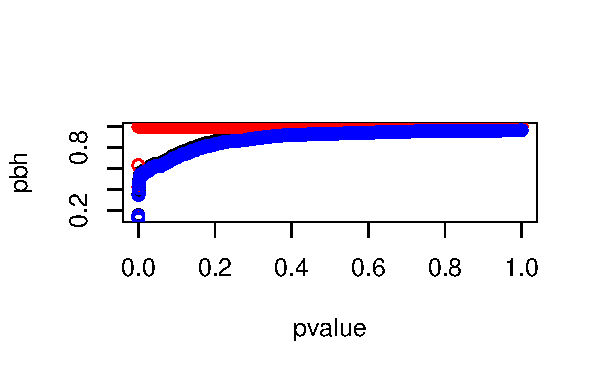
\includegraphics{sciguide_files/figure-latex/unnamed-chunk-13-1}

此时我们可以看到两者结果较为接近,q值理论上更完备,功效也更强,但算法上对\(\hat\pi_0\)的估计并不稳定,特别是比例靠近1的时候,所以BH方法可能还是更容易让人接受的保守错误发现率控制。详细的估计方法还得去啃Storey的\href{http://www.pnas.org/content/100/16/9440.full}{论文}。

多重检验问题是高通量数据里逃不掉的问题,要想找出真正的差异数据就要面对假阳性跟假阴性问题,这是一个不可兼得的过程,看重假阳性就用整体错误率,看重功效就用错误发现率控制。并不是说哪种方法会好一些,更本质的问题在于你对实际问题的了解程度及统计方法的适用范围。例如你选基因芯片时实际也进行了一次选择,改变了整体检验的p值分布,而不同的p值分布对应的处理方法也不太一样,有兴趣可以读下\href{http://varianceexplained.org/statistics/interpreting-pvalue-histogram/}{这篇}。有时候你的实验设计本身就会影响数据的统计行为,而这个恰恰是最容易被忽视的。

\hypertarget{ux7ebfux6027ux6a21ux578b}{%
\section{线性模型}\label{ux7ebfux6027ux6a21ux578b}}

\begin{itemize}
\tightlist
\item
  从lasso到岭回归,惩罚项在回归分析中的应用
\item
  截断回归与缺失值处理
\item
  线性混合模型
\item
  线性模型中非考察变量的判定与消除
\item
  分层模型 \url{https://www.nature.com/articles/nbt.1619}
\item
  线性判别分析与特征发现
\item
  logistic回归与剂量效应曲线
\item
  相关性分析与工具变量 \url{https://www.nature.com/articles/nbt0309-255}
\item
  偏最小二乘分析在结构效应关系研究中的应用
\item
  非线性模型包括凸函数与凹函数
\item
  最常见凸函数是指数函数,掌握72法制,也就是72除以速率大概就是翻倍用的时间
\item
  最常见凹函数是收益递减函数,平均价值大于价值的平均,具有风险规避特性
\item
  劳动力和资本凹函数,新的投资得到的收益会越来越低
\end{itemize}

\hypertarget{ux8ba1ux7b97ux65b9ux6cd5}{%
\section{计算方法}\label{ux8ba1ux7b97ux65b9ux6cd5}}

\hypertarget{ux5e76ux884cux8ba1ux7b97}{%
\subsection{并行计算}\label{ux5e76ux884cux8ba1ux7b97}}

\hypertarget{ux96c6ux7fa4ux8ba1ux7b97}{%
\subsection{集群计算}\label{ux96c6ux7fa4ux8ba1ux7b97}}

\hypertarget{ux5bb9ux5668ux6280ux672f}{%
\subsection{容器技术}\label{ux5bb9ux5668ux6280ux672f}}

\hypertarget{ux4e91ux8ba1ux7b97}{%
\subsection{云计算}\label{ux4e91ux8ba1ux7b97}}

\hypertarget{ux4effux771fux6a21ux62df}{%
\subsection{仿真模拟}\label{ux4effux771fux6a21ux62df}}

\begin{itemize}
\tightlist
\item
  bootstrap思想
\item
  ABM
\item
  MCMC方法
\end{itemize}

\hypertarget{ux5e38ux89c1ux7b97ux6cd5}{%
\section{常见算法}\label{ux5e38ux89c1ux7b97ux6cd5}}

\begin{itemize}
\item
  MCMC方法 \url{https://www.nature.com/articles/nbt1004-1315}
\item
  聚类与主成分分析 \url{https://www.nature.com/articles/nbt0308-303} \url{https://www.nature.com/articles/nbt1205-1499}
\item
  列联表分析与流行病学研究
\item
  人工神经网络与黑箱计算 \url{http://www.nature.com/doifinder/10.1038/nbt1386}
\item
  支持向量机的回归与分类 \url{https://www.nature.com/articles/nbt1206-1565}
\item
  从决策树到随机森林 \url{http://www.nature.com/doifinder/10.1038/nbt0908-1011}
\item
  经验贝叶斯与近似贝叶斯计算(ABC)及贝叶斯网络 \url{https://www.nature.com/articles/nbt0106-51}
  \url{https://www.nature.com/articles/nbt0806-959}
  \url{https://www.nature.com/articles/nbt0904-1177}
\item
  时间序列分析
\item
  结构方程模型
\item
  动态规划 \url{https://www.nature.com/articles/nbt0704-909}
\end{itemize}

\hypertarget{lib}{%
\chapter{文献}\label{lib}}

\hypertarget{ux6587ux732eux7ba1ux7406}{%
\section{文献管理}\label{ux6587ux732eux7ba1ux7406}}

文献管理方面主要包括文献收集、整理、分析与追踪,目的是获取当前研究趋势。用认知过程阶段可以分成三个:从无到有、从有到精与从精到用,从无到有是指刚进入一个新领域时的状态,绝大多数研究生跟转行的科研人员都要通过这个阶段构建自己的文献知识库;从有到精指维护与整理与追踪新文献;从精到用阶段指文献知识库体系直接参与科研过程形成产出的过程。

\hypertarget{ux4eceux65e0ux5230ux6709}{%
\subsection{从无到有}\label{ux4eceux65e0ux5230ux6709}}

刚开展研究工作的第一步就是背景知识的了解,除非你研究生转行,一般本科阶段的学习应该已经掌握了学科基础,这个是共通的背景知识。基于此你要从教科书上相对确定的知识走向文献资料中相对不那么确定的知识,此时最好的开端是一本英文教材,一方面锻炼英文,另一方面英文教材的更新比国内要快(你大概率可以从图书馆借到,而且多数图书馆都有根据你需求订书的服务,不要浪费)。如果你精力足够,甚至可以联系作者问下是否可以翻译,这样一举多得,不过我没操作过,只是建议。另一个思路是通过 MOOCs 来系统学习,国内外很多高校放到网上的课程授课老师都属于接受新思想比较快的人,讲义也比较前沿,系统性比较高。还有一个不太通用的方法是阅读近些年的博士论文,其文献部分一般都是相关信息,不过能不能找到就不好说了。这个阶段一般要两三个月,不要心急,先把基础打好。前面掉的坑越多,后面跳坑就更有经验。

一般而言,一项学术成果要先发表,然后被综述评论,然后进入研究生课程讨论班,然后进入本科生课程讲义,最后才进入学科经典教材的更新。所以你可以倒着去走这个流程,越往后可能越不容易懂,但循序渐进总比一下读前沿论文被搞晕要好。有了相对前沿的教材或讲义作为知识框架,你的脑子里此时应该比较清楚导师让你做的东西或自己打算做的东西在学科中的定位,解决的是什么科学或工程问题,此时可以进行基于关键词检索的文献收集了。

一个良好的搜索返回的结果应该在10篇以内,首先要是综述,然后关键词检索方面建议学点逻辑运算符来过滤掉不相关信息,如果你上一阶段看的书是5年前更新的,那就只去关注最近5年的综述;如果你做的领域实在太新,那就把关键词信息的同义词跟近义词也加到搜索里;如果你能找到一篇写的特别好的综述或者有高人指点的论文,那是最高效的方法,可遇不可求。这10篇论文请按年为单位每1-2年选一篇综述去看,一月内读完,要求是精读,也就是论文里提到的研究都加到你的文献库里并阅读细节,同时可参考综述章节对文献库进行分组。一定要做笔记,而且要进行结构化的笔记或思维导图,这个阶段时间可能比较长也比较累,成果是当你去听系里的报告时,你大概能将报告定位到你的笔记框架里。到此文献库就从无到有了。

\hypertarget{ux4eceux6709ux5230ux7cbe}{%
\subsection{从有到精}\label{ux4eceux6709ux5230ux7cbe}}

有了文献库不代表就不用读了,你要建立一个体系来整理并追踪最新文献,这一阶段希望你早就了解 RSS 是怎么回事并且使用过 RSS 阅读器。如果没有,邮件订阅也不失为一个良方。这里我要提示一下,一般文献库管理工具都提供针对单篇文献的笔记功能,不要用。请自建按研究主题的笔记,把新的有意思的新论文连同你以后可能引用的语句直接摘到相关主题的笔记里,而且要让你的笔记可以反链到数据库或通过 doi 可以直接找到原文(推荐后者)。没别的意思,我希望你的笔记稍加整理就可以作为综述发表,省的你次次重返工。建议文献追新频率每周一次,固定时间,看到好的文章就马上消化掉。

\hypertarget{ux4eceux7cbeux5230ux7528}{%
\subsection{从精到用}\label{ux4eceux7cbeux5230ux7528}}

文献信息的收集与整理不是为了写笔记,是为了需要用的时候瞬间能够用到,例如写一个技术报告,给别人审稿,还有最重要的:写科技论文。科技论文不同于其他文体一个最显著的特点就是参考文献体系的支撑:所有的讨论都要起于前人的发现,参考文献事实上经常是考察作者知识面的关键,对前人工作的遗漏会严重降低文章的系统性与创新性,经常会被审稿人一票否决,哪怕其实你做的跟前人是不一样的。另外的使用就是报告幻灯片跟其他学术交流场景,如果你能做到在大脑或笔记中快速定位到一个观点或现象然后几句话说清楚,这个习惯能帮你离开学术界后在其他行业直接展开降维打击。绝大多数离开学术界的人都不会继续保持了解前沿动态的习惯而更多依赖过往经验,一个人的经验如何去抗衡一堆参考文献背后成百上千人的经验?当然有些东西那些成百上千人也许都不知道,特别是工程上的。不过这种``学院派''的研究习惯最大的好处就是让人更谦逊些,知道一山更比一山高,处处重峦叠嶂。那些上来就趾高气昂且沉醉于自己小圈子的人,不管在学术界还是其他行业,九成以上是鼠目寸光之辈,请远离这些人。

谈文献管理,我希望不要掉到工具选择的坑里,要构建完整的知识管理体系,哪怕是基于便签的只要能实现头脑知识的更新换代就可以了,如果能方便写作投稿,那就更好了。切不可舍本逐末,单纯把文章发表作为目标去优化,毕竟所有的短期目标都要最终整合成你学术生涯的一部分,可以抽时间去想想一些简单的问题:

\begin{itemize}
\tightlist
\item
  我的研究究竟有没有实际意义?
\item
  我的发现是否有助于学科发展或写入教科书?
\item
  我现在纠结的事10年20年后会不会纠结?
\end{itemize}

以人之渺小,所有的时间都是浪费,但你要为自己浪费的时光赋值。

\hypertarget{ux4fe1ux606fux6536ux96c6}{%
\section{信息收集}\label{ux4fe1ux606fux6536ux96c6}}

文献信息要采用被动收集来获得实时更新,被动收集就是通过加入邮件列表、新闻组或订阅期刊或数据库关键词的 RSS 来完成。信息收集有三个层次,最低就是关键词相关文献,这个主要依赖 RSS 或追踪重点课题组,关注这个可以保证对自己研究方向的掌握,不仅是期刊论文,预印本与会议论文也要关注到;中间层就是专业类顶级期刊,关注这部分信息可以对学科发展趋势有所了解;如果还有时间精力,可以关注综合类期刊,例如nature、pnas、science、NEJM、JAMA等,了解重大科学问题。

阅读文献时,要合理分配时间,科技文献已经\href{https://www.alternet.org/news-amp-politics/science-has-outgrown-human-mind-and-its-limited-capacities-process-information}{超越}了人脑处理信息的能力了。一般而言都要读题目, 20-50\%读摘要,5-10\%看图,1-3\%读全文。网上一般都可以找到摘要,如果需要全文,可以在 twitter 上用 \#icanhazpdf 找、可以用\href{https://github.com/ropensci/fulltext}{fulltext}包找、可以用 \href{https://unpaywall.org/}{unpaywall} 的 API \href{https://cran.r-project.org/web/packages/roadoi/vignettes/intro.html}{找}、可以用\href{https://openaccessbutton.org/}{Open Access Button}的 API 来找、当然也可以找作者要或者找有权限的朋友帮忙。

文献管理软件方面有收费的也有免费的,一般而言可通过咨询自己所在科研机构的图书馆来获取是否购买了相应的软件,一般图书馆也提供使用培训。早期文献管理软件之间差异还是明显的,但到今天基本同质化了。

\hypertarget{ux6587ux732eux5f15ux7528}{%
\section{文献引用}\label{ux6587ux732eux5f15ux7528}}

文献的收集是为了使用,科研中最主要使用文献的场景就是论文写作,当你想参考别人的研究结论或研究数据时,一般会在相应位置插入参考文献(引文)。然后,在论文的结尾或章节页面结尾要对引用过的参考文献进行列表,方便读者按图索骥。引文与列表要有定位功能,引文要有对应列表展示题录信息,列表要保证读者可以根据期刊、作者等信息可检索到原始文献。现在很多出版商都会提供富文本的论文,里面的参考文献都可以直接链接到原文网页,当然作者不必要实现这个功能,但作者一般要保证自己初稿是符合待投期刊格式的,这些在投稿指南中都会写的很清楚。

如何保证引用符合格式要求是研究人员要注意的,期刊格式要求其实主要就是限定页面布局与参考文献格式,主流期刊会提供 Word 文档模版与 LaTeX 宏包两种方式,前者很难限定参考文献格式,后者使用难度很高,都是要配合文献管理软件的对应插件来实现。文献排版的底层逻辑是在插入文献时在论文里生成一个针对该文献的锚点,当编译或格式化时,通过锚点查找你文献库(一般是独立的文件保存,不同文献管理软件不一样,bib文件相对通用性好些)里的题录信息,然后按照特定格式要求生成论文里的引文与文末的文献列表。引文有时是数字,有时是人名与年份,一般都很简短;文献列表信息量更大些,更方便读者查找源头,格式与排序不同期刊的要求也差距很大。

其实,每篇文章的题录都可以生成特定值,甚至直接就是原文链接,具象化的产物就是 DOI ,你可以通过文章的 DOI 指纹与在线数据转换接口快速得到更丰富的信息。现代科研里,文献列表的信息越来越不如网站链接便利,可以设想未来的期刊应该主要是网页版,且引文可以通过超链接互通,这样的学术交流效果应该是最好的。不过,眼下我们还是要遵照期刊要求投稿,不过现在期刊对于格式的要求已经因为自动化排版流程而越来越少,科研工作者可以把精力更多放在内容生产上而非手工整理格式,效率低且错误率高。

\hypertarget{ux6587ux672cux6316ux6398}{%
\section{文本挖掘}\label{ux6587ux672cux6316ux6398}}

我们可以借助文本挖掘的工具来探索大量文献中的趋势,这对快速了解某期刊或某关键词的学术界研究趋势很有帮助,也可以作为论文前言的论据。文本挖掘不依赖逐字逐篇阅读文献,更多是依赖文献标题或摘要甚至全文中词汇的词频与相关性等统计指标来推测研究趋势。

文本挖掘目前技术上虽然成熟但精度上并不高,要谨慎使用该技术。一般而言,文本挖掘的时间跨度不超过10年且最好5年以内,因为综述跨度一般不超过10年,可以直接依赖10年内出版的综述来了解研究现状。在实战上,我们可以直接使用支持自然语言学习的统计软件来进行文本挖掘,也可以通过文献信息学软件来做,前提是准备好搜索语句或文献题录库。这里我们用案例来理解下这种文献分析方法。

\hypertarget{ux5173ux952eux8bcd}{%
\subsection{关键词}\label{ux5173ux952eux8bcd}}

以关键词为核心的文本挖掘旨在寻找所有该关键词相关研究的时间变化趋势与相关子领域。技术上首先利用关键词去寻找在线文摘数据库中的论文题录,然后提取摘要部分进行分词并统计词频。这里我们用``mass spectrometry''作为关键词搜索2010到2020年间发表在 ES\&T 上的论文做演示。

\begin{Shaded}
\begin{Highlighting}[]
\KeywordTok{library}\NormalTok{(scifetch)}
\KeywordTok{library}\NormalTok{(lubridate)}
\KeywordTok{library}\NormalTok{(dplyr)}
\KeywordTok{library}\NormalTok{(tidytext)}
\KeywordTok{library}\NormalTok{(stringr)}
\KeywordTok{library}\NormalTok{(ggplot2)}
\KeywordTok{library}\NormalTok{(tidyr)}
\KeywordTok{library}\NormalTok{(broom)}
\KeywordTok{library}\NormalTok{(purrr)}
\KeywordTok{library}\NormalTok{(scales)}
\CommentTok{# 10年跨度 MeSH 关键词 期刊ES&T}
\NormalTok{query <-}\StringTok{ "}\CharTok{\textbackslash{}"}\StringTok{mass spectrometry}\CharTok{\textbackslash{}"}\StringTok{[MeSH Terms] AND 2010/01:2020/01[DP] AND 0013-936X[TA]"}
\NormalTok{tmdf <-}\StringTok{ }\KeywordTok{getpubmed}\NormalTok{(query, }\DataTypeTok{start =} \DecValTok{1}\NormalTok{, }\DataTypeTok{end =} \DecValTok{10000}\NormalTok{) }\OperatorTok\StringTok{ }\KeywordTok{getpubmedtbl}\NormalTok{() }\OperatorTok\StringTok{ }
\StringTok{    }\KeywordTok{mutate}\NormalTok{(}\DataTypeTok{time =} \KeywordTok{as.POSIXct}\NormalTok{(date, }\DataTypeTok{origin =} \StringTok{"1970-01-01"}\NormalTok{), }\DataTypeTok{month =} \KeywordTok{round_date}\NormalTok{(date, }
        \StringTok{"month"}\NormalTok{))}
\end{Highlighting}
\end{Shaded}

\begin{verbatim}
## 822 records founds
\end{verbatim}

\begin{Shaded}
\begin{Highlighting}[]
\CommentTok{# 摘要分词}
\NormalTok{wordfabs <-}\StringTok{ }\NormalTok{tmdf }\OperatorTok\StringTok{ }\KeywordTok{filter}\NormalTok{(}\KeywordTok{nchar}\NormalTok{(abstract) }\OperatorTok{>}\StringTok{ }\DecValTok{0}\NormalTok{) }\OperatorTok\StringTok{ }\KeywordTok{unnest_tokens}\NormalTok{(word, }
\NormalTok{    abstract, }\DataTypeTok{drop =}\NormalTok{ F) }\OperatorTok\StringTok{ }\KeywordTok{anti_join}\NormalTok{(stop_words) }\OperatorTok\StringTok{ }\KeywordTok{filter}\NormalTok{(}\KeywordTok{str_detect}\NormalTok{(word, }
    \StringTok{"[^}\CharTok{\textbackslash{}\textbackslash{}}\StringTok{d]"}\NormalTok{)) }\OperatorTok\StringTok{ }\KeywordTok{filter}\NormalTok{(}\OperatorTok{!}\KeywordTok{str_detect}\NormalTok{(word, }\StringTok{"abs"}\NormalTok{)) }\OperatorTok\StringTok{ }\KeywordTok{group_by}\NormalTok{(word) }\OperatorTok\StringTok{ }
\StringTok{    }\KeywordTok{mutate}\NormalTok{(}\DataTypeTok{word_total =} \KeywordTok{n}\NormalTok{()) }\OperatorTok\StringTok{ }\KeywordTok{ungroup}\NormalTok{() }\OperatorTok\StringTok{ }\KeywordTok{mutate}\NormalTok{(}\DataTypeTok{source =} \StringTok{"abstract"}\NormalTok{)}
\end{Highlighting}
\end{Shaded}

\begin{verbatim}
## Joining, by = "word"
\end{verbatim}

\begin{Shaded}
\begin{Highlighting}[]
\CommentTok{# 可视化词频前20的关键词}
\NormalTok{wordfabs }\OperatorTok\StringTok{ }\KeywordTok{count}\NormalTok{(word, }\DataTypeTok{sort =} \OtherTok{TRUE}\NormalTok{) }\OperatorTok\StringTok{ }\KeywordTok{top_n}\NormalTok{(}\DecValTok{20}\NormalTok{, n) }\OperatorTok\StringTok{ }\KeywordTok{mutate}\NormalTok{(}\DataTypeTok{word =} \KeywordTok{reorder}\NormalTok{(word, }
\NormalTok{    n)) }\OperatorTok\StringTok{ }\KeywordTok{ggplot}\NormalTok{(}\KeywordTok{aes}\NormalTok{(word, n)) }\OperatorTok{+}\StringTok{ }\KeywordTok{geom_col}\NormalTok{(}\DataTypeTok{show.legend =} \OtherTok{FALSE}\NormalTok{) }\OperatorTok{+}\StringTok{ }
\StringTok{    }\KeywordTok{ylab}\NormalTok{(}\StringTok{"Top 20 commonly used words in abstracts"}\NormalTok{) }\OperatorTok{+}\StringTok{ }\KeywordTok{coord_flip}\NormalTok{()}
\end{Highlighting}
\end{Shaded}

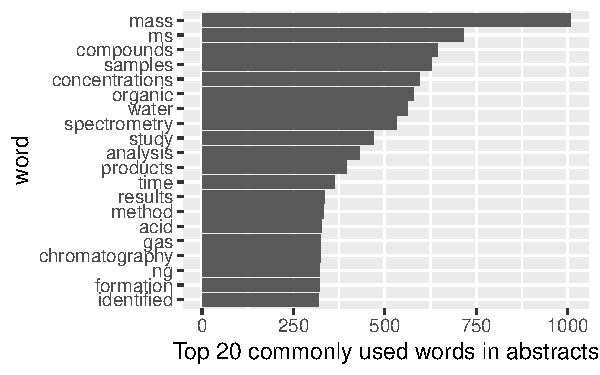
\includegraphics{sciguide_files/figure-latex/unnamed-chunk-14-1}

同时我们可以看下这10年关键词的变化趋势。

\begin{Shaded}
\begin{Highlighting}[]
\NormalTok{papers_per_month <-}\StringTok{ }\NormalTok{tmdf }\OperatorTok\StringTok{ }\KeywordTok{group_by}\NormalTok{(month) }\OperatorTok\StringTok{ }\KeywordTok{summarize}\NormalTok{(}\DataTypeTok{month_total =} \KeywordTok{n}\NormalTok{())}
\end{Highlighting}
\end{Shaded}

\begin{verbatim}
## `summarise()` ungrouping output (override with `.groups` argument)
\end{verbatim}

\begin{Shaded}
\begin{Highlighting}[]
\CommentTok{# 摘要中关键词}
\NormalTok{word_month_counts <-}\StringTok{ }\NormalTok{wordfabs }\OperatorTok\StringTok{ }\KeywordTok{filter}\NormalTok{(word_total }\OperatorTok{>=}\StringTok{ }\DecValTok{100}\NormalTok{) }\OperatorTok\StringTok{ }
\StringTok{    }\KeywordTok{count}\NormalTok{(word, month) }\OperatorTok\StringTok{ }\KeywordTok{complete}\NormalTok{(word, month, }\DataTypeTok{fill =} \KeywordTok{list}\NormalTok{(}\DataTypeTok{n =} \DecValTok{0}\NormalTok{)) }\OperatorTok\StringTok{ }
\StringTok{    }\KeywordTok{inner_join}\NormalTok{(papers_per_month, }\DataTypeTok{by =} \StringTok{"month"}\NormalTok{) }\OperatorTok\StringTok{ }\KeywordTok{mutate}\NormalTok{(}\DataTypeTok{percent =}\NormalTok{ n}\OperatorTok{/}\NormalTok{month_total) }\OperatorTok\StringTok{ }
\StringTok{    }\KeywordTok{mutate}\NormalTok{(}\DataTypeTok{year =} \KeywordTok{year}\NormalTok{(month) }\OperatorTok{+}\StringTok{ }\KeywordTok{yday}\NormalTok{(month)}\OperatorTok{/}\DecValTok{365}\NormalTok{) }\OperatorTok\StringTok{ }\KeywordTok{filter}\NormalTok{(percent }\OperatorTok{<}\StringTok{ }
\StringTok{    }\DecValTok{1}\NormalTok{)}
\CommentTok{# 计数数据广义二项回归}
\NormalTok{mod <-}\StringTok{ }\ErrorTok{~}\KeywordTok{glm}\NormalTok{(}\KeywordTok{cbind}\NormalTok{(n, month_total }\OperatorTok{-}\StringTok{ }\NormalTok{n) }\OperatorTok{~}\StringTok{ }\NormalTok{year, ., }\DataTypeTok{family =} \StringTok{"binomial"}\NormalTok{)}
\CommentTok{# 计算斜率}
\NormalTok{slopes <-}\StringTok{ }\NormalTok{word_month_counts }\OperatorTok\StringTok{ }\KeywordTok{nest}\NormalTok{(}\OperatorTok{-}\NormalTok{word) }\OperatorTok\StringTok{ }\KeywordTok{mutate}\NormalTok{(}\DataTypeTok{model =} \KeywordTok{map}\NormalTok{(data, }
\NormalTok{    mod)) }\OperatorTok\StringTok{ }\KeywordTok{mutate}\NormalTok{(}\DataTypeTok{models =} \KeywordTok{map}\NormalTok{(model, tidy)) }\OperatorTok\StringTok{ }\KeywordTok{unnest}\NormalTok{(}\DataTypeTok{cols =} \KeywordTok{c}\NormalTok{(models)) }\OperatorTok\StringTok{ }
\StringTok{    }\KeywordTok{filter}\NormalTok{(term }\OperatorTok{==}\StringTok{ "year"}\NormalTok{) }\OperatorTok\StringTok{ }\KeywordTok{arrange}\NormalTok{(}\KeywordTok{desc}\NormalTok{(estimate))}
\end{Highlighting}
\end{Shaded}

\begin{verbatim}
## Warning: All elements of `...` must be named.
## Did you want `data = c(month, n, month_total, percent, year)`?
\end{verbatim}

\begin{Shaded}
\begin{Highlighting}[]
\CommentTok{# 快速成长关键词}
\NormalTok{slopes }\OperatorTok\StringTok{ }\KeywordTok{head}\NormalTok{(}\DecValTok{9}\NormalTok{) }\OperatorTok\StringTok{ }\KeywordTok{inner_join}\NormalTok{(word_month_counts, }\DataTypeTok{by =} \StringTok{"word"}\NormalTok{) }\OperatorTok\StringTok{ }
\StringTok{    }\KeywordTok{mutate}\NormalTok{(}\DataTypeTok{word =} \KeywordTok{reorder}\NormalTok{(word, }\OperatorTok{-}\NormalTok{estimate)) }\OperatorTok\StringTok{ }\KeywordTok{ggplot}\NormalTok{(}\KeywordTok{aes}\NormalTok{(month, }
\NormalTok{    n}\OperatorTok{/}\NormalTok{month_total, }\DataTypeTok{color =}\NormalTok{ word)) }\OperatorTok{+}\StringTok{ }\KeywordTok{geom_line}\NormalTok{(}\DataTypeTok{show.legend =} \OtherTok{FALSE}\NormalTok{) }\OperatorTok{+}\StringTok{ }
\StringTok{    }\KeywordTok{scale_y_continuous}\NormalTok{(}\DataTypeTok{labels =} \KeywordTok{percent_format}\NormalTok{()) }\OperatorTok{+}\StringTok{ }\KeywordTok{facet_wrap}\NormalTok{(}\OperatorTok{~}\NormalTok{word, }
    \DataTypeTok{scales =} \StringTok{"free_y"}\NormalTok{) }\OperatorTok{+}\StringTok{ }\KeywordTok{expand_limits}\NormalTok{(}\DataTypeTok{y =} \DecValTok{0}\NormalTok{) }\OperatorTok{+}\StringTok{ }\KeywordTok{labs}\NormalTok{(}\DataTypeTok{x =} \StringTok{"Year"}\NormalTok{, }
    \DataTypeTok{y =} \StringTok{"Percentage of abstracts containing this term"}\NormalTok{, }\DataTypeTok{title =} \StringTok{"9 fastest growing words"}\NormalTok{, }
    \DataTypeTok{subtitle =} \StringTok{"Judged by growth rate"}\NormalTok{)}
\end{Highlighting}
\end{Shaded}

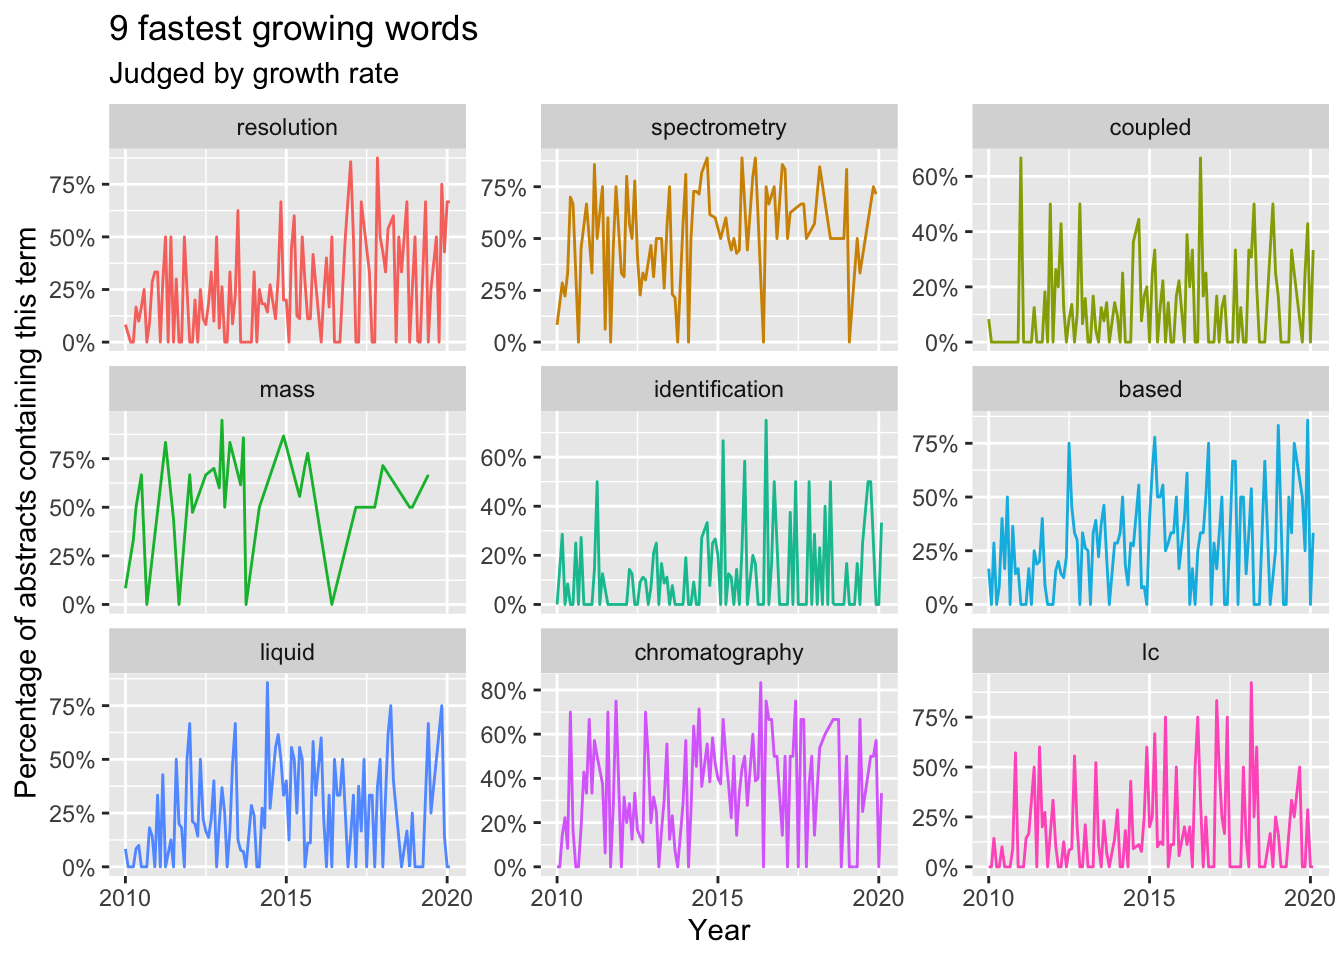
\includegraphics{sciguide_files/figure-latex/unnamed-chunk-15-1}

\begin{Shaded}
\begin{Highlighting}[]
\CommentTok{# 衰退关键词}
\NormalTok{slopes }\OperatorTok\StringTok{ }\KeywordTok{tail}\NormalTok{(}\DecValTok{9}\NormalTok{) }\OperatorTok\StringTok{ }\KeywordTok{inner_join}\NormalTok{(word_month_counts, }\DataTypeTok{by =} \StringTok{"word"}\NormalTok{) }\OperatorTok\StringTok{ }
\StringTok{    }\KeywordTok{mutate}\NormalTok{(}\DataTypeTok{word =} \KeywordTok{reorder}\NormalTok{(word, estimate)) }\OperatorTok\StringTok{ }\KeywordTok{ggplot}\NormalTok{(}\KeywordTok{aes}\NormalTok{(month, }
\NormalTok{    n}\OperatorTok{/}\NormalTok{month_total, }\DataTypeTok{color =}\NormalTok{ word)) }\OperatorTok{+}\StringTok{ }\KeywordTok{geom_line}\NormalTok{(}\DataTypeTok{show.legend =} \OtherTok{FALSE}\NormalTok{) }\OperatorTok{+}\StringTok{ }
\StringTok{    }\KeywordTok{scale_y_continuous}\NormalTok{(}\DataTypeTok{labels =} \KeywordTok{percent_format}\NormalTok{()) }\OperatorTok{+}\StringTok{ }\KeywordTok{facet_wrap}\NormalTok{(}\OperatorTok{~}\NormalTok{word, }
    \DataTypeTok{scales =} \StringTok{"free_y"}\NormalTok{) }\OperatorTok{+}\StringTok{ }\KeywordTok{expand_limits}\NormalTok{(}\DataTypeTok{y =} \DecValTok{0}\NormalTok{) }\OperatorTok{+}\StringTok{ }\KeywordTok{labs}\NormalTok{(}\DataTypeTok{x =} \StringTok{"Year"}\NormalTok{, }
    \DataTypeTok{y =} \StringTok{"Percentage of abstracts containing this term"}\NormalTok{, }\DataTypeTok{title =} \StringTok{"9 fastest shrinking words"}\NormalTok{, }
    \DataTypeTok{subtitle =} \StringTok{"Judged by growth rate"}\NormalTok{)}
\end{Highlighting}
\end{Shaded}

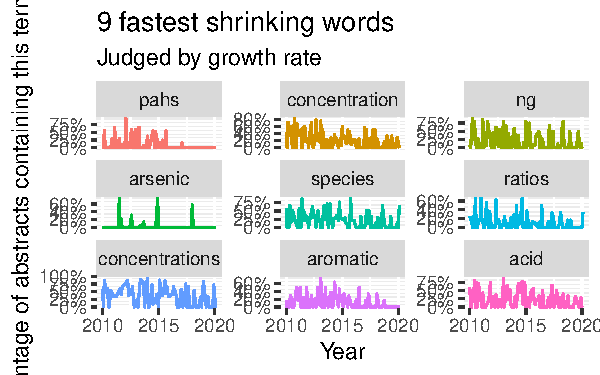
\includegraphics{sciguide_files/figure-latex/unnamed-chunk-15-2}

同时,我们也可以利用词频相关来研究关键词聚类情况。

\begin{Shaded}
\begin{Highlighting}[]
\KeywordTok{library}\NormalTok{(widyr)}
\KeywordTok{library}\NormalTok{(igraph)}
\KeywordTok{library}\NormalTok{(ggraph)}

\NormalTok{title_word_pairs <-}\StringTok{ }\NormalTok{wordfabs }\OperatorTok\StringTok{ }\KeywordTok{pairwise_count}\NormalTok{(word, line, }\DataTypeTok{sort =} \OtherTok{TRUE}\NormalTok{)}

\KeywordTok{set.seed}\NormalTok{(}\DecValTok{42}\NormalTok{)}
\NormalTok{title_word_pairs }\OperatorTok\StringTok{ }\KeywordTok{filter}\NormalTok{(n }\OperatorTok{>=}\StringTok{ }\DecValTok{150}\NormalTok{) }\OperatorTok\StringTok{ }\KeywordTok{graph_from_data_frame}\NormalTok{() }\OperatorTok\StringTok{ }
\StringTok{    }\KeywordTok{ggraph}\NormalTok{(}\DataTypeTok{layout =} \StringTok{"fr"}\NormalTok{) }\OperatorTok{+}\StringTok{ }\KeywordTok{geom_edge_link}\NormalTok{(}\KeywordTok{aes}\NormalTok{(}\DataTypeTok{edge_alpha =}\NormalTok{ n, }
    \DataTypeTok{edge_width =}\NormalTok{ n), }\DataTypeTok{edge_colour =} \StringTok{"cyan4"}\NormalTok{) }\OperatorTok{+}\StringTok{ }\KeywordTok{geom_node_point}\NormalTok{(}\DataTypeTok{size =} \DecValTok{1}\NormalTok{) }\OperatorTok{+}\StringTok{ }
\StringTok{    }\KeywordTok{geom_node_text}\NormalTok{(}\KeywordTok{aes}\NormalTok{(}\DataTypeTok{label =}\NormalTok{ name), }\DataTypeTok{repel =} \OtherTok{TRUE}\NormalTok{, }\DataTypeTok{point.padding =} \KeywordTok{unit}\NormalTok{(}\FloatTok{0.2}\NormalTok{, }
        \StringTok{"lines"}\NormalTok{)) }\OperatorTok{+}\StringTok{ }\KeywordTok{labs}\NormalTok{(}\DataTypeTok{title =} \StringTok{"Bigrams in title"}\NormalTok{) }\OperatorTok{+}\StringTok{ }\KeywordTok{theme_void}\NormalTok{()}
\end{Highlighting}
\end{Shaded}

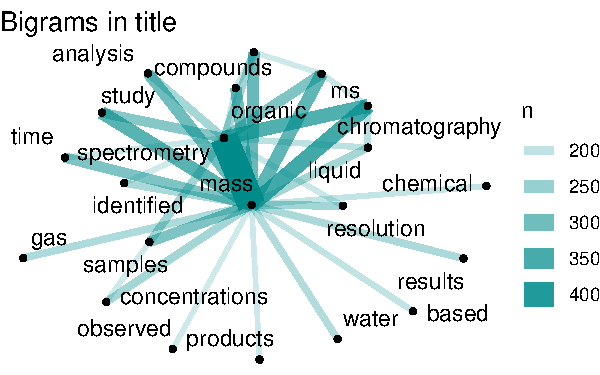
\includegraphics{sciguide_files/figure-latex/unnamed-chunk-16-1}

更直接的方法是用主题模型来寻找子领域,例如我们可以指定6个子领域输出其前10关键词。

\begin{Shaded}
\begin{Highlighting}[]
\NormalTok{desc_dtm <-}\StringTok{ }\NormalTok{wordfabs }\OperatorTok\StringTok{ }\KeywordTok{count}\NormalTok{(line, word, }\DataTypeTok{sort =} \OtherTok{TRUE}\NormalTok{) }\OperatorTok\StringTok{ }\KeywordTok{ungroup}\NormalTok{() }\OperatorTok\StringTok{ }
\StringTok{    }\KeywordTok{cast_dtm}\NormalTok{(line, word, n)}
\KeywordTok{library}\NormalTok{(topicmodels)}
\NormalTok{desc_lda <-}\StringTok{ }\KeywordTok{LDA}\NormalTok{(desc_dtm, }\DataTypeTok{k =} \DecValTok{6}\NormalTok{, }\DataTypeTok{control =} \KeywordTok{list}\NormalTok{(}\DataTypeTok{seed =} \DecValTok{42}\NormalTok{))}
\NormalTok{tidy_lda <-}\StringTok{ }\KeywordTok{tidy}\NormalTok{(desc_lda)}

\NormalTok{top_terms <-}\StringTok{ }\NormalTok{tidy_lda }\OperatorTok\StringTok{ }\KeywordTok{group_by}\NormalTok{(topic) }\OperatorTok\StringTok{ }\KeywordTok{top_n}\NormalTok{(}\DecValTok{10}\NormalTok{, beta) }\OperatorTok\StringTok{ }
\StringTok{    }\KeywordTok{ungroup}\NormalTok{() }\OperatorTok\StringTok{ }\KeywordTok{arrange}\NormalTok{(topic, }\OperatorTok{-}\NormalTok{beta)}

\NormalTok{top_terms }\OperatorTok\StringTok{ }\KeywordTok{mutate}\NormalTok{(}\DataTypeTok{term =} \KeywordTok{reorder}\NormalTok{(term, beta)) }\OperatorTok\StringTok{ }\KeywordTok{group_by}\NormalTok{(topic, }
\NormalTok{    term) }\OperatorTok\StringTok{ }\KeywordTok{arrange}\NormalTok{(}\KeywordTok{desc}\NormalTok{(beta)) }\OperatorTok\StringTok{ }\KeywordTok{ungroup}\NormalTok{() }\OperatorTok\StringTok{ }\KeywordTok{mutate}\NormalTok{(}\DataTypeTok{term =} \KeywordTok{factor}\NormalTok{(}\KeywordTok{paste}\NormalTok{(term, }
\NormalTok{    topic, }\DataTypeTok{sep =} \StringTok{"__"}\NormalTok{), }\DataTypeTok{levels =} \KeywordTok{rev}\NormalTok{(}\KeywordTok{paste}\NormalTok{(term, topic, }\DataTypeTok{sep =} \StringTok{"__"}\NormalTok{)))) }\OperatorTok\StringTok{ }
\StringTok{    }\KeywordTok{ggplot}\NormalTok{(}\KeywordTok{aes}\NormalTok{(term, beta, }\DataTypeTok{fill =} \KeywordTok{as.factor}\NormalTok{(topic))) }\OperatorTok{+}\StringTok{ }\KeywordTok{geom_col}\NormalTok{(}\DataTypeTok{show.legend =} \OtherTok{FALSE}\NormalTok{) }\OperatorTok{+}\StringTok{ }
\StringTok{    }\KeywordTok{coord_flip}\NormalTok{() }\OperatorTok{+}\StringTok{ }\KeywordTok{scale_x_discrete}\NormalTok{(}\DataTypeTok{labels =} \ControlFlowTok{function}\NormalTok{(x) }\KeywordTok{gsub}\NormalTok{(}\StringTok{"__.+$"}\NormalTok{, }
    \StringTok{""}\NormalTok{, x)) }\OperatorTok{+}\StringTok{ }\KeywordTok{labs}\NormalTok{(}\DataTypeTok{title =} \StringTok{"Top 10 terms in each LDA topic"}\NormalTok{, }
    \DataTypeTok{x =} \OtherTok{NULL}\NormalTok{, }\DataTypeTok{y =} \KeywordTok{expression}\NormalTok{(beta)) }\OperatorTok{+}\StringTok{ }\KeywordTok{facet_wrap}\NormalTok{(}\OperatorTok{~}\NormalTok{topic, }\DataTypeTok{ncol =} \DecValTok{2}\NormalTok{, }
    \DataTypeTok{scales =} \StringTok{"free"}\NormalTok{)}
\end{Highlighting}
\end{Shaded}

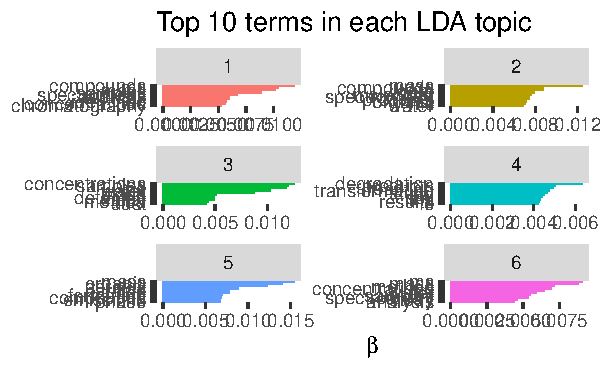
\includegraphics{sciguide_files/figure-latex/unnamed-chunk-17-1}

\hypertarget{ux4f5cux8005}{%
\subsection{作者}\label{ux4f5cux8005}}

同样的,我们也可以研究某个作者的研究主题与变化趋势。这里用加拿大滑铁卢大学 Jaunsz Pawliszyn 教授的数据来说明下。

\begin{Shaded}
\begin{Highlighting}[]
\CommentTok{# 10年跨度}
\NormalTok{query <-}\StringTok{ "janusz pawliszyn[AU] AND 2010/01:2020/01[DP]"}
\NormalTok{tmdf <-}\StringTok{ }\KeywordTok{getpubmed}\NormalTok{(query, }\DataTypeTok{start =} \DecValTok{1}\NormalTok{, }\DataTypeTok{end =} \DecValTok{10000}\NormalTok{) }\OperatorTok\StringTok{ }\KeywordTok{getpubmedtbl}\NormalTok{() }\OperatorTok\StringTok{ }
\StringTok{    }\KeywordTok{mutate}\NormalTok{(}\DataTypeTok{time =} \KeywordTok{as.POSIXct}\NormalTok{(date, }\DataTypeTok{origin =} \StringTok{"1970-01-01"}\NormalTok{), }\DataTypeTok{month =} \KeywordTok{round_date}\NormalTok{(date, }
        \StringTok{"month"}\NormalTok{))}
\end{Highlighting}
\end{Shaded}

\begin{verbatim}
## 195 records founds
\end{verbatim}

\begin{Shaded}
\begin{Highlighting}[]
\CommentTok{# 摘要分词}
\NormalTok{wordfabs <-}\StringTok{ }\NormalTok{tmdf }\OperatorTok\StringTok{ }\KeywordTok{filter}\NormalTok{(}\KeywordTok{nchar}\NormalTok{(abstract) }\OperatorTok{>}\StringTok{ }\DecValTok{0}\NormalTok{) }\OperatorTok\StringTok{ }\KeywordTok{unnest_tokens}\NormalTok{(word, }
\NormalTok{    abstract, }\DataTypeTok{drop =}\NormalTok{ F) }\OperatorTok\StringTok{ }\KeywordTok{anti_join}\NormalTok{(stop_words) }\OperatorTok\StringTok{ }\KeywordTok{filter}\NormalTok{(}\KeywordTok{str_detect}\NormalTok{(word, }
    \StringTok{"[^}\CharTok{\textbackslash{}\textbackslash{}}\StringTok{d]"}\NormalTok{)) }\OperatorTok\StringTok{ }\KeywordTok{filter}\NormalTok{(}\OperatorTok{!}\KeywordTok{str_detect}\NormalTok{(word, }\StringTok{"abs"}\NormalTok{)) }\OperatorTok\StringTok{ }\KeywordTok{group_by}\NormalTok{(word) }\OperatorTok\StringTok{ }
\StringTok{    }\KeywordTok{mutate}\NormalTok{(}\DataTypeTok{word_total =} \KeywordTok{n}\NormalTok{()) }\OperatorTok\StringTok{ }\KeywordTok{ungroup}\NormalTok{() }\OperatorTok\StringTok{ }\KeywordTok{mutate}\NormalTok{(}\DataTypeTok{source =} \StringTok{"abstract"}\NormalTok{)}
\end{Highlighting}
\end{Shaded}

\begin{verbatim}
## Joining, by = "word"
\end{verbatim}

\begin{Shaded}
\begin{Highlighting}[]
\NormalTok{papers_per_month <-}\StringTok{ }\NormalTok{tmdf }\OperatorTok\StringTok{ }\KeywordTok{group_by}\NormalTok{(month) }\OperatorTok\StringTok{ }\KeywordTok{summarize}\NormalTok{(}\DataTypeTok{month_total =} \KeywordTok{n}\NormalTok{())}
\end{Highlighting}
\end{Shaded}

\begin{verbatim}
## `summarise()` ungrouping output (override with `.groups` argument)
\end{verbatim}

\begin{Shaded}
\begin{Highlighting}[]
\CommentTok{# 可视化词频前20的关键词}
\NormalTok{wordfabs }\OperatorTok\StringTok{ }\KeywordTok{count}\NormalTok{(word, }\DataTypeTok{sort =} \OtherTok{TRUE}\NormalTok{) }\OperatorTok\StringTok{ }\KeywordTok{top_n}\NormalTok{(}\DecValTok{20}\NormalTok{, n) }\OperatorTok\StringTok{ }\KeywordTok{mutate}\NormalTok{(}\DataTypeTok{word =} \KeywordTok{reorder}\NormalTok{(word, }
\NormalTok{    n)) }\OperatorTok\StringTok{ }\KeywordTok{ggplot}\NormalTok{(}\KeywordTok{aes}\NormalTok{(word, n)) }\OperatorTok{+}\StringTok{ }\KeywordTok{geom_col}\NormalTok{(}\DataTypeTok{show.legend =} \OtherTok{FALSE}\NormalTok{) }\OperatorTok{+}\StringTok{ }
\StringTok{    }\KeywordTok{ylab}\NormalTok{(}\StringTok{"Top 20 commonly used words in abstracts"}\NormalTok{) }\OperatorTok{+}\StringTok{ }\KeywordTok{coord_flip}\NormalTok{()}
\end{Highlighting}
\end{Shaded}

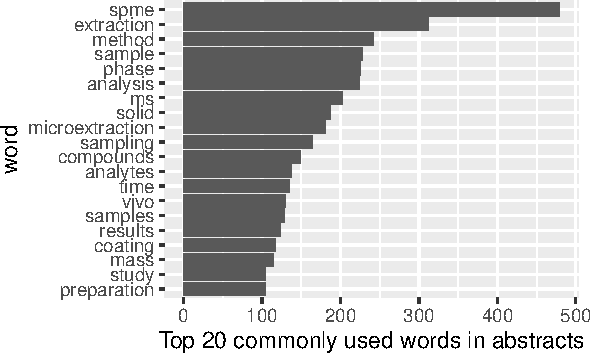
\includegraphics{sciguide_files/figure-latex/unnamed-chunk-18-1}

\begin{Shaded}
\begin{Highlighting}[]
\CommentTok{# 摘要中关键词}
\NormalTok{word_month_counts <-}\StringTok{ }\NormalTok{wordfabs }\OperatorTok\StringTok{ }\KeywordTok{filter}\NormalTok{(word_total }\OperatorTok{>=}\StringTok{ }\DecValTok{100}\NormalTok{) }\OperatorTok\StringTok{ }
\StringTok{    }\KeywordTok{count}\NormalTok{(word, month) }\OperatorTok\StringTok{ }\KeywordTok{complete}\NormalTok{(word, month, }\DataTypeTok{fill =} \KeywordTok{list}\NormalTok{(}\DataTypeTok{n =} \DecValTok{0}\NormalTok{)) }\OperatorTok\StringTok{ }
\StringTok{    }\KeywordTok{inner_join}\NormalTok{(papers_per_month, }\DataTypeTok{by =} \StringTok{"month"}\NormalTok{) }\OperatorTok\StringTok{ }\KeywordTok{mutate}\NormalTok{(}\DataTypeTok{percent =}\NormalTok{ n}\OperatorTok{/}\NormalTok{month_total) }\OperatorTok\StringTok{ }
\StringTok{    }\KeywordTok{mutate}\NormalTok{(}\DataTypeTok{year =} \KeywordTok{year}\NormalTok{(month) }\OperatorTok{+}\StringTok{ }\KeywordTok{yday}\NormalTok{(month)}\OperatorTok{/}\DecValTok{365}\NormalTok{) }\OperatorTok\StringTok{ }\KeywordTok{filter}\NormalTok{(percent }\OperatorTok{<}\StringTok{ }
\StringTok{    }\DecValTok{1}\NormalTok{)}
\CommentTok{# 计数数据广义二项回归}
\NormalTok{mod <-}\StringTok{ }\ErrorTok{~}\KeywordTok{glm}\NormalTok{(}\KeywordTok{cbind}\NormalTok{(n, month_total }\OperatorTok{-}\StringTok{ }\NormalTok{n) }\OperatorTok{~}\StringTok{ }\NormalTok{year, ., }\DataTypeTok{family =} \StringTok{"binomial"}\NormalTok{)}
\CommentTok{# 计算斜率}
\NormalTok{slopes <-}\StringTok{ }\NormalTok{word_month_counts }\OperatorTok\StringTok{ }\KeywordTok{nest}\NormalTok{(}\OperatorTok{-}\NormalTok{word) }\OperatorTok\StringTok{ }\KeywordTok{mutate}\NormalTok{(}\DataTypeTok{model =} \KeywordTok{map}\NormalTok{(data, }
\NormalTok{    mod)) }\OperatorTok\StringTok{ }\KeywordTok{mutate}\NormalTok{(}\DataTypeTok{models =} \KeywordTok{map}\NormalTok{(model, tidy)) }\OperatorTok\StringTok{ }\KeywordTok{unnest}\NormalTok{(}\DataTypeTok{cols =} \KeywordTok{c}\NormalTok{(models)) }\OperatorTok\StringTok{ }
\StringTok{    }\KeywordTok{filter}\NormalTok{(term }\OperatorTok{==}\StringTok{ "year"}\NormalTok{) }\OperatorTok\StringTok{ }\KeywordTok{arrange}\NormalTok{(}\KeywordTok{desc}\NormalTok{(estimate))}
\end{Highlighting}
\end{Shaded}

\begin{verbatim}
## Warning: All elements of `...` must be named.
## Did you want `data = c(month, n, month_total, percent, year)`?
\end{verbatim}

\begin{Shaded}
\begin{Highlighting}[]
\CommentTok{# 快速成长关键词}
\NormalTok{slopes }\OperatorTok\StringTok{ }\KeywordTok{head}\NormalTok{(}\DecValTok{9}\NormalTok{) }\OperatorTok\StringTok{ }\KeywordTok{inner_join}\NormalTok{(word_month_counts, }\DataTypeTok{by =} \StringTok{"word"}\NormalTok{) }\OperatorTok\StringTok{ }
\StringTok{    }\KeywordTok{mutate}\NormalTok{(}\DataTypeTok{word =} \KeywordTok{reorder}\NormalTok{(word, }\OperatorTok{-}\NormalTok{estimate)) }\OperatorTok\StringTok{ }\KeywordTok{ggplot}\NormalTok{(}\KeywordTok{aes}\NormalTok{(month, }
\NormalTok{    n}\OperatorTok{/}\NormalTok{month_total, }\DataTypeTok{color =}\NormalTok{ word)) }\OperatorTok{+}\StringTok{ }\KeywordTok{geom_line}\NormalTok{(}\DataTypeTok{show.legend =} \OtherTok{FALSE}\NormalTok{) }\OperatorTok{+}\StringTok{ }
\StringTok{    }\KeywordTok{scale_y_continuous}\NormalTok{(}\DataTypeTok{labels =} \KeywordTok{percent_format}\NormalTok{()) }\OperatorTok{+}\StringTok{ }\KeywordTok{facet_wrap}\NormalTok{(}\OperatorTok{~}\NormalTok{word, }
    \DataTypeTok{scales =} \StringTok{"free_y"}\NormalTok{) }\OperatorTok{+}\StringTok{ }\KeywordTok{expand_limits}\NormalTok{(}\DataTypeTok{y =} \DecValTok{0}\NormalTok{) }\OperatorTok{+}\StringTok{ }\KeywordTok{labs}\NormalTok{(}\DataTypeTok{x =} \StringTok{"Year"}\NormalTok{, }
    \DataTypeTok{y =} \StringTok{"Percentage of abstracts containing this term"}\NormalTok{, }\DataTypeTok{title =} \StringTok{"9 fastest growing words"}\NormalTok{, }
    \DataTypeTok{subtitle =} \StringTok{"Judged by growth rate"}\NormalTok{)}
\end{Highlighting}
\end{Shaded}

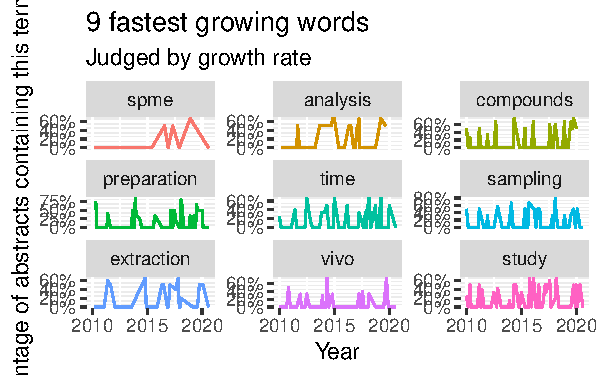
\includegraphics{sciguide_files/figure-latex/unnamed-chunk-18-2}

\begin{Shaded}
\begin{Highlighting}[]
\CommentTok{# 衰退关键词}
\NormalTok{slopes }\OperatorTok\StringTok{ }\KeywordTok{tail}\NormalTok{(}\DecValTok{9}\NormalTok{) }\OperatorTok\StringTok{ }\KeywordTok{inner_join}\NormalTok{(word_month_counts, }\DataTypeTok{by =} \StringTok{"word"}\NormalTok{) }\OperatorTok\StringTok{ }
\StringTok{    }\KeywordTok{mutate}\NormalTok{(}\DataTypeTok{word =} \KeywordTok{reorder}\NormalTok{(word, estimate)) }\OperatorTok\StringTok{ }\KeywordTok{ggplot}\NormalTok{(}\KeywordTok{aes}\NormalTok{(month, }
\NormalTok{    n}\OperatorTok{/}\NormalTok{month_total, }\DataTypeTok{color =}\NormalTok{ word)) }\OperatorTok{+}\StringTok{ }\KeywordTok{geom_line}\NormalTok{(}\DataTypeTok{show.legend =} \OtherTok{FALSE}\NormalTok{) }\OperatorTok{+}\StringTok{ }
\StringTok{    }\KeywordTok{scale_y_continuous}\NormalTok{(}\DataTypeTok{labels =} \KeywordTok{percent_format}\NormalTok{()) }\OperatorTok{+}\StringTok{ }\KeywordTok{facet_wrap}\NormalTok{(}\OperatorTok{~}\NormalTok{word, }
    \DataTypeTok{scales =} \StringTok{"free_y"}\NormalTok{) }\OperatorTok{+}\StringTok{ }\KeywordTok{expand_limits}\NormalTok{(}\DataTypeTok{y =} \DecValTok{0}\NormalTok{) }\OperatorTok{+}\StringTok{ }\KeywordTok{labs}\NormalTok{(}\DataTypeTok{x =} \StringTok{"Year"}\NormalTok{, }
    \DataTypeTok{y =} \StringTok{"Percentage of abstracts containing this term"}\NormalTok{, }\DataTypeTok{title =} \StringTok{"9 fastest shrinking words"}\NormalTok{, }
    \DataTypeTok{subtitle =} \StringTok{"Judged by growth rate"}\NormalTok{)}
\end{Highlighting}
\end{Shaded}

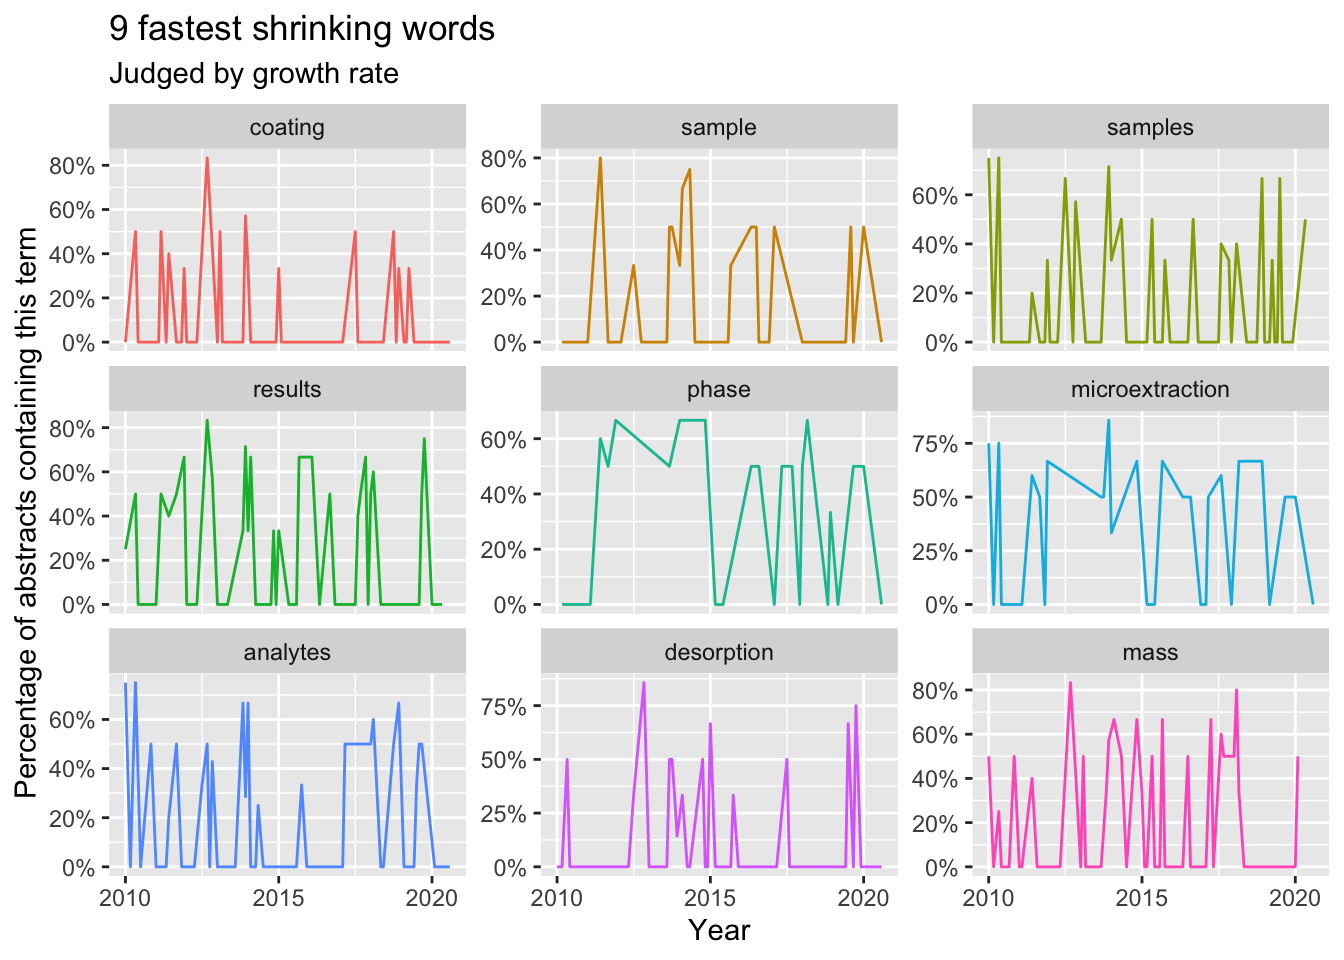
\includegraphics{sciguide_files/figure-latex/unnamed-chunk-18-3}

同样,我们可以研究下其发表的期刊偏好。

\begin{Shaded}
\begin{Highlighting}[]
\KeywordTok{table}\NormalTok{(tmdf}\OperatorTok{$}\NormalTok{journal)[}\KeywordTok{order}\NormalTok{(}\KeywordTok{table}\NormalTok{(tmdf}\OperatorTok{$}\NormalTok{journal), }\DataTypeTok{decreasing =}\NormalTok{ T)][}\DecValTok{1}\OperatorTok{:}\DecValTok{10}\NormalTok{]}
\end{Highlighting}
\end{Shaded}

\begin{verbatim}
## 
##                 Anal. Chem.            Anal. Chim. Acta 
##                          44                          33 
##              J Chromatogr A                 Bioanalysis 
##                          32                           9 
##      Environ. Sci. Technol.                   J Sep Sci 
##                           7                           7 
## Angew. Chem. Int. Ed. Engl.                     Sci Rep 
##                           6                           6 
##                     Talanta                     Analyst 
##                           6                           4
\end{verbatim}

\hypertarget{ux671fux520a}{%
\subsection{期刊}\label{ux671fux520a}}

期刊也可以用上述分析来研究期刊偏好与学科发展趋势。

\hypertarget{ux6587ux732eux4fe1ux606fux5b66}{%
\section{文献信息学}\label{ux6587ux732eux4fe1ux606fux5b66}}

专门的文献信息学工具也可以拿来进行学术趋势的挖掘,因为文献题录是高度结构化的数据,所以文献间关系可以用结构化数据来构建联系。基于引用关系我们可以找到某个关键词或期刊的节点论文。引用也可以跟文本分析相联系,用来寻找高引论文的文本写作风格。而基于研究人员的时空分布我们可以评估研究国际化与合作水平。文献信息学中也有专门的指标用来评估研究趋势或文章/学者影响力,可了解相关概念与使用,但不要过度解读与依赖,学科前沿并不稳定,量化指标通常只能描述一部分趋势。

\hypertarget{ux835fux8403ux5206ux6790}{%
\section{荟萃分析}\label{ux835fux8403ux5206ux6790}}

荟萃分析常用来对已发表的实验结果进行二次分析得到一个更全面的结论,常用于心理学、流行病学与经济学研究等。其应用场景通常是想回答一个被重复研究过的科学问题,例如某种疾病在不同人群中的风险比等。不过,不同实验精度不同、样本量不同、方差不同、效应也会不同,此时荟萃分析就可以用来汇总出一个关于结论的结论,本质上是一个层级模型。

荟萃分析有两种基本模型,一种是固定效应模型,一种是随机效应模型。前者只有确认不同研究都针对同一群体时才适合用,然而绝大多数情况下不同研究的群体是不一样的,因此实际使用中随机效应模型用的更多,因为其考虑了不同研究自身的随机性。

固定效应模型对总效应的估计是基于对不同研究方差的倒数加权来计算的,也就是说研究的标准误越高,其对总效应的贡献就越小,具体公式是:

\[\hat\theta_F = \frac{\sum\limits_{k=1}^K \hat\theta_k/ \hat\sigma^2_k}{\sum\limits_{k=1}^K 1/\hat\sigma^2_k}\]

如果样本存在异质性,那么就要用随机效应模型。在随机效应模型中,我们假设每一研究给出的效应来自于一个分布而不是固定的值,这样我们就还要估计这个分布的不确定度,一般用 \texttt{\$\textbackslash{}tau\^{}2\$} 来表示。同时,效应可以是连续变量,也可以是二元变量,也可以是类似相关系数的统计量。

荟萃分析的结果通常用森林图来表示,上面会列上单独研究的效应估计及置信区间、权重,也会给出整体效应估计与置信区间。同时,一般荟萃分析的软件也会给出异质性系数及对该系数的假设检验结果,也会给出预测区间。如果异质性系数低于 25\% ,我们会认为可以直接用固定效应模型,如果高于75\%,则异质性非常大。预测区间给出的是基于当前荟萃分析结果未来研究效应可能出现的区间,通常比估计效应的置信区间要大,但回答的不是一个问题,估计效应的置信区间描述得是多次重复实验后在一定置信水平下真值会出现的区间。

在荟萃分析中,有些个别研究可能对整体估计产生较大影响,所以要进行敏感度分析或影响分析,通常敏感度分析是用留一法来做的,也就是排除掉这个研究去重新估计效应,看前后差距是否显著,如果显著最好排除掉。

有时荟萃分析中研究可以进一步分类,此时可以引入混合效应模型,也就是各分类效应固定,但各分类效应的误差来自于一个分布。同时研究中涉及的变量如果不是分类而是连续变量,那么也可以进行荟萃回归分析,同样可以做固定效应模型与混合效应模型。

荟萃分析中一个重要主题就是发表歧视,小样本研究通常可信度要低于大样本但容易获得明显效应。漏斗图常用来表示不同效应及标准误的汇聚程度,根据对称性检验(Egger's test)我们可以推测哪些研究结果可能存在发表歧视。另一种发表歧视的检验方法是汇总分析 p 值的分布,如果真实效应存在则应该是左偏的,而不是汇聚到 0.05 附近。

荟萃分析还可以进一步通过对研究质量进行定量后汇总评价,主要用来展示不同操作步骤引入的不确定性。更为复杂的荟萃分析会去考虑不同处理间的直接与间接影响,一般是通过网络分析来进行。同理,这类存在层级结构的分析问题也可以通过结构方程模型来求解,寻找出观察层背后的潜在结构。

可以参考\href{https://bookdown.org/MathiasHarrer/Doing_Meta_Analysis_in_R/}{这}\href{https://ebmh.bmj.com/content/ebmental/22/4/153.full.pdf}{里}进行更多荟萃分析的实战。

\hypertarget{life}{%
\chapter{学术生活}\label{life}}

\hypertarget{ux5b66ux672fux9053ux5fb7ux4f26ux7406}{%
\section{学术道德/伦理}\label{ux5b66ux672fux9053ux5fb7ux4f26ux7406}}

\hypertarget{ux527dux7a83}{%
\subsection{剽窃}\label{ux527dux7a83}}

剽窃(plagiarism)包括但不限于对他人发表或未发表工作、想法、数据等的不恰当引用或故意不引用,也包括对自己发表成果的重复使用。在引述别人观点时,要做到总结转述与引用同时使用以表示对原作者的致敬。整段引用可使用引号但要根据期刊要求来做,转述不能简单做语序调整与同义词互换,要做到理解层面的叙述。对于别人在学术交流场合进行的讨论,也要进行充分引用来说明来源,学术圈里人们不会因为想法是你的而尊敬你多少,但会因为想法不是你的你却说成是自己的而鄙视你。

\hypertarget{ux6587ux7ae0ux6302ux540d}{%
\subsection{文章挂名}\label{ux6587ux7ae0ux6302ux540d}}

尽早决定且只有对文章有显著智力非物质贡献的人适合挂名,在现实中会存在索要挂名的行为但需要综合考虑。一般来说,挂名作者要至少有如下行为之一:

\begin{itemize}
\tightlist
\item
  提出概念或设计
\item
  收集分析数据
\item
  撰写草稿
\item
  同意最终版本发表并负责
\end{itemize}

不得不承认的是有些人可能仅仅是在文章写作阶段参与,但其对文章的内容理解阐述可以让读者很简单了解文章的内容,此时是否列入作者需要综合考虑而不是单纯排斥,每篇文章都有自己的生命力而不是私产。当然请编辑润稿不在其中,因为编辑不对内容负责。影子作者或者代笔是严格禁止的。对于吉祥物作者,请知会该作者并阐明挂名风险,能成为吉祥物的资深研究人员有能力对自己的名誉风险做判断。各个领域的要求可能不同,但很简单的方法就是文章列一个作者贡献章节,详细记录每个挂名作者的贡献。

除了挂名,致谢中表示物质援助与技术援助也是一种不错的致敬方式,在感谢前,请告知他们并获取同意许可。

文章挂名的另一个问题是作者排序,常规操作是资深研究人员放在最后,第一作者是文章主要撰写人。作者排序常常由资深研究人员来决定,因为他们对全局智力贡献把握更准确,但最好做到内部透明。如果智力贡献不多,做实验最多的人有可能不被列为第一作者,对于研究生而言,请不要把体力劳动当成第一作者的保险,请一定参与数据分析与文章撰写磨练自己的科研能力。有些领域例如物理学会按字母表来进行作者排序,但并未广泛推广。个人认为比较理性的情况是作者字母排序配合致谢与贡献章节来解决挂名问题。

\hypertarget{ux53ccux91cdux53d1ux8868}{%
\subsection{双重发表}\label{ux53ccux91cdux53d1ux8868}}

一稿两投严格禁止,这对同行评议期刊的自愿审稿资源是浪费,也是不尊重。但双重发表在以下情况可能是允许的:

\begin{itemize}
\tightlist
\item
  翻译
\item
  在选集中发表
\item
  文章受众不同
\item
  期刊间交流透明并对著作权无异议
\end{itemize}

\hypertarget{ux6570ux636eux9020ux5047}{%
\subsection{数据造假}\label{ux6570ux636eux9020ux5047}}

伪造(fabrication)是通过创造数据来论证自己想要的答案。修改图片,用仿真数据充当真实数据等方式都属于伪造。伪造可通过统计手段来检验。

篡改(falsification)是通过对真实数据进行修改来论证自己想要的答案。这种比单纯伪造要难发现,但独立实验室验证会发现问题。

\hypertarget{ux6709ux5bb3ux7814ux7a76ux5b9eux8df5}{%
\subsection{有害研究实践}\label{ux6709ux5bb3ux7814ux7a76ux5b9eux8df5}}

有害研究实践(detrimental research practices)指的是一些不易界定的学术不端,例如使用错误的统计方法与实验设计,故意隐瞒阴性结果及不披露利益冲突。

\hypertarget{ux4e0dux5408ux89c4}{%
\subsection{不合规}\label{ux4e0dux5408ux89c4}}

不合规(Noncompliance)指的是违法政策法规的研究,通常涉及伦理问题。

\hypertarget{ux6027ux9a9aux6270}{%
\subsection{性骚扰}\label{ux6027ux9a9aux6270}}

学术界性骚扰也是学术不端的一种形式,除了道德法律政策不允许外还会直接影响实验可信度。

\hypertarget{ux4f26ux7406}{%
\subsection{伦理}\label{ux4f26ux7406}}

广义科研伦理包括不限于正直(说话算数可信)、诚实(不弄虚作假)、透明(可披露研究非隐私细节)、能力(专业性)、合作(能与人共事进行研究)、社会责任、服从法律法规公义与责任心。科研人员不能在伦理问题上出问题,否则会断送职业生涯。

\hypertarget{ux9879ux76eeux7ba1ux7406}{%
\section{项目管理}\label{ux9879ux76eeux7ba1ux7406}}

\hypertarget{ux9999ux80a0ux6218ux672f}{%
\subsection{香肠战术}\label{ux9999ux80a0ux6218ux672f}}

\begin{itemize}
\item
  不断切分到具体可执行
\item
  执行成本可控
\item
  执行时不思考整体,关注当下
\item
  转移注意力可放松,但要设计成杨白劳模式
\item
  分阶段有始有终
\item
  \href{https://www.allthingsdistributed.com/2006/11/working_backwards.html}{向后工作法}
  1、写新闻稿
  2、写 FAQ
  3、写用户文档
  4、写代码
\end{itemize}

\hypertarget{ux98ceux9669ux7ba1ux7406}{%
\subsection{风险管理}\label{ux98ceux9669ux7ba1ux7406}}

\begin{itemize}
\tightlist
\item
  有应急预案设计
\item
  对外界环境变化有列表
\item
  安全优先原则
\end{itemize}

\hypertarget{ux65f6ux95f4ux7ba1ux7406}{%
\subsection{时间管理}\label{ux65f6ux95f4ux7ba1ux7406}}

\begin{itemize}
\tightlist
\item
  开立多个项目,保证时间都浪费在有意义的事上
\item
  整体统筹进度控制与甘特图
\item
  增值分析
\item
  紧急重要四象限
\item
  与未来自己博弈
\end{itemize}

\hypertarget{ux601dux7ef4ux5bfcux56fe}{%
\subsection{思维导图}\label{ux601dux7ef4ux5bfcux56fe}}

\begin{itemize}
\tightlist
\item
  构建知识体系
\end{itemize}

\hypertarget{ux5934ux8111ux98ceux66b4}{%
\subsection{头脑风暴}\label{ux5934ux8111ux98ceux66b4}}

\begin{itemize}
\tightlist
\item
  随意去想相关答案
\item
  将答案按工作量与影响力进行区分
\item
  选取工作量低但影响力大的方案
\end{itemize}

\hypertarget{swotux5206ux6790}{%
\subsection{SWOT分析}\label{swotux5206ux6790}}

\begin{itemize}
\tightlist
\item
  列举自己技术的优势与劣势
\item
  列举外部环境的机会与威胁
\item
  对内外进行组合,设置对策,优势机会要扩张,劣势机会要补充不足,优势威胁要有预案,劣势威胁要对冲风险
\end{itemize}

\hypertarget{ux7b14ux8bb0ux7ba1ux7406}{%
\subsection{笔记管理}\label{ux7b14ux8bb0ux7ba1ux7406}}

\begin{itemize}
\tightlist
\item
  版本控制
\item
  定期回顾
\item
  \href{https://zh.wikipedia.org/wiki/\%E5\%BA\%B7\%E5\%A5\%88\%E5\%B0\%94\%E7\%AC\%94\%E8\%AE\%B0\%E6\%B3\%95}{康奈尔笔记法}
\item
  晨间日记管理自己
\item
  费曼学习法,通过教或写文章总结来学
\end{itemize}

\hypertarget{ux90aeux4ef6}{%
\subsection{邮件}\label{ux90aeux4ef6}}

\begin{itemize}
\tightlist
\item
  回复要快,24小时以内
\item
  题目要有辨识度,简明扼要
\item
  题目/正文要有关键词方便检索
\item
  一封邮件讨论一件事
\item
  简短,让读者有可操作性
\item
  时间紧急时告诉收信人无回复的结果
\item
  有后续追踪
\item
  有附件一定在正文中说明
\item
  提供自己联系方式
\item
  尽量纯文本文件
\item
  抄送的人没有回复义务
\item
  注意回复一个人还是所有人
\item
  秘密抄送尽量不要用
\item
  收到回信根据落款选择下一次名字
\item
  给陌生人邮件第一句介绍自己
\item
  第二句介绍你如何直到对方
\item
  不用 I wanted 或 I would like,用 I was wondering
\item
  可使用列表
\item
  避免 please
\item
  检查拼写
\item
  结尾表示感谢
\item
  落款可用 Sincerely,Best wishes
\end{itemize}

\hypertarget{ux5b66ux672fux51faux7248}{%
\section{学术出版}\label{ux5b66ux672fux51faux7248}}

\hypertarget{ux671fux520aux8bbaux6587}{%
\subsection{期刊论文}\label{ux671fux520aux8bbaux6587}}

\begin{itemize}
\item
  合作者人数与版本控制
\item
  先画图后写作

  \begin{itemize}
  \tightlist
  \item
    可视化陷阱
  \item
    模块化制图
  \end{itemize}
\item
  语言简洁可能不利于发表,但有利于传播
\item
  公开代码、数据、软件来提高研究的可重复性,被重复有利于提高学术影响力
\item
  信任合作者
\item
  马上动笔,拒绝完美
\item
  博客文章、软件包在传播上与论文一样重要,甚至更重要
\item
  论文由方法、数据、结果跟结论组成,先完成前三个
\item
  阴性结果也是结果,对其他科研人员也有参考价值,也要考虑发表,哪怕是博客发表
\item
  预先发表 \href{https://deevybee.blogspot.com/2018/06/preprint-publication-as-karaoke.html}{资料}
\item
  投稿到你设想中读者会读到的地方
\item
  通过社交网络传播你的发现
\item
  开放获取???基金与影响力传播
\item
  延长论文的半衰期
\item
  \href{https://rayyan.qcri.org}{综述}
\item
  回复审稿人

  \begin{itemize}
  \tightlist
  \item
    逐条回复
  \item
    指明文中修改的位置
  \end{itemize}
\end{itemize}

\hypertarget{ux4f1aux8baeux6458ux8981}{%
\subsection{会议摘要}\label{ux4f1aux8baeux6458ux8981}}

\hypertarget{ux4e13ux8457}{%
\subsection{专著}\label{ux4e13ux8457}}

\begin{itemize}
\tightlist
\item
  在线出版
\item
  允许反馈
\item
  leanpub/gitbook/amazon kindle direct publishing/bookdown
\item
  按需求出版纸质版 lulu.com
\end{itemize}

\hypertarget{ux4e13ux5229}{%
\subsection{专利}\label{ux4e13ux5229}}

\hypertarget{ux8f6fux4ef6}{%
\subsection{软件}\label{ux8f6fux4ef6}}

\begin{itemize}
\tightlist
\item
  \href{https://simplystatistics.org/2018/05/03/software-as-an-academic-publication/}{软件就是发表}
\item
  \href{http://joss.theoj.org/}{JOSS}
\end{itemize}

\hypertarget{ux5b66ux672fux4f1aux8bae}{%
\section{学术会议}\label{ux5b66ux672fux4f1aux8bae}}

\hypertarget{ux53e3ux5934ux62a5ux544a}{%
\subsection{口头报告}\label{ux53e3ux5934ux62a5ux544a}}

\begin{itemize}
\tightlist
\item
  提前到场交流
\item
  娱乐而不是教诲
\item
  写给观众而不是自己
\item
  用所见即所得方式
\item
  首页末页有联系方式
\item
  大字体
\item
  有链接
\item
  对比色
\item
  图片文字比1000:1
\item
  解释图片时先说干什么用的,然后解释坐标,然后解释关键现象
\item
  解释公式时用文字不要用单一符号,脚标不要太多
\item
  注意时间 1-2 分钟一张幻灯片
\item
  报告后写邮件感谢组织者
\end{itemize}

\hypertarget{ux6d77ux62a5ux62a5ux544a}{%
\subsection{海报报告}\label{ux6d77ux62a5ux62a5ux544a}}

\begin{itemize}
\tightlist
\item
  减少文字描述,使用条目来概括研究
\item
  从左到右,从上到下的阅读顺序
\item
  信息图可以加分,但比较费精力
\item
  使用 \href{https://www.insidehighered.com/news/2019/06/24/theres-movement-better-scientific-posters-are-they-really-better}{betterposter} 设计风格:左侧表示研究细节,中间放关键词加大加粗的结论配上论文QR码,右侧放回答问题所需要的图表,制作时间可以极大缩短,用色块来提高识别度
\item
  使用 \href{https://derekcrowe.net/butterposter}{butterpoposter} 设计风格:上述风格的改进版,引入图形摘要,标题占右上1/4,右下是图形摘要,左边是模块化的高亮点或细节
\end{itemize}

\hypertarget{ux7535ux68afux62a5ux544a}{%
\subsection{电梯报告}\label{ux7535ux68afux62a5ux544a}}

\begin{itemize}
\tightlist
\item
  elevator pitch,一分钟甚至三十秒来报告你的研究或引发兴趣
\end{itemize}

\hypertarget{ux542cux62a5ux544a}{%
\subsection{听报告}\label{ux542cux62a5ux544a}}

\begin{itemize}
\tightlist
\item
  携带名片
\item
  记笔记或录音,当天消化,邮件追踪
\item
  礼貌交流
\item
  提问题不要讲自己的故事
\item
  不要问与学术无关的事
\end{itemize}

\hypertarget{ux5ba1ux7a3f}{%
\section{审稿}\label{ux5ba1ux7a3f}}

\begin{itemize}
\tightlist
\item
  1665年伦敦皇家学会出版《The Philosophical Transactions of the Royal Society of London》,巴黎科学院出版《Journal des Scavans》,这是最早两份学术期刊
\item
  1752年伦敦皇家学会意识到有些文章质量不高,开始启用同行评议
\item
  1830s 皇家协会正式引入同行评议来控制文章质量
\item
  1937年,美国国立癌症研究所首先启用同行评议来评审基金,后逐渐流行
\item
  审稿分为开方式、单盲(主流)与双盲三种
\item
  尽快,否则不做
\item
  可以进行发表后审稿或公开评论
\item
  流程是主编确认投稿是否合乎范围,分配给专业副主编,副主编寻找审稿人
\item
  如果对方改了也不能达到你认为的标准,拒绝而不是大修或小修
\item
  不要在审稿意见中推广自己的观点,就事论事
\item
  \href{https://doi.org/10.1371/journal.pone.0026895}{开放审稿会提高同行评议准确率}
\item
  \href{https://doi.org/10.1021/ez5001148}{审稿指数}
\end{itemize}

\hypertarget{ux5b66ux672fux5408ux4f5c}{%
\section{学术合作}\label{ux5b66ux672fux5408ux4f5c}}

学术合作有三种形式,学术圈内合作、学术圈-业界合作、学术圈-社区合作。业界合作是被允许的但会有系统偏差,集中于营利。社区合作通常需要社区配合采集数据,成果也服务于社区。跨国界合作需要遵守所有研究机构的要求才能进行,要提前打招呼,并有相关备忘。

\hypertarget{ux5229ux76caux51b2ux7a81}{%
\section{利益冲突}\label{ux5229ux76caux51b2ux7a81}}

\begin{itemize}
\tightlist
\item
  影响主观判断的经济或其他利益或不公平的竞争优势
\item
  利益冲突在研究项目进行过程中随时会出现,要及时申报或停止项目,等待审核
\item
  经济利益冲突不仅包括研究人员个体与业界的利益关系,还可能是通过机构资助而存在的潜在利益关系
\item
  非经济利益冲突主包括确认偏误,也就研究中只发表对自己有利的结果,也包括良心冲突,如与军方合作的项目,更包括个人利益冲突,例如工作机会等
\item
  承诺冲突指在不同工作间存在的干扰,特别是对首要雇主(通常是研究机构)的干扰。例如一个学生为老师做研究助理的同时也在老师的公司兼职就会有承诺冲突问题,需要跟研究机构申报,而这位老师也存在学生研究成果私用的利益冲突问题
\item
  利益冲突会引入系统偏见、对已有研究结果的质疑、损害研究机构声誉与获得基金的机会
\item
  利益冲突需要提高透明度来解决,并消除利益冲突的影响
\end{itemize}

\hypertarget{ux6570ux636eux5171ux4eab}{%
\subsection{数据共享}\label{ux6570ux636eux5171ux4eab}}

\begin{itemize}
\tightlist
\item
  通过学科内流行平台实现
\item
  一定要有文档解释编号
\item
  使用开源格式与许可
\end{itemize}

\hypertarget{ux793eux4ea4ux7f51ux7edc}{%
\subsection{社交网络}\label{ux793eux4ea4ux7f51ux7edc}}

\begin{itemize}
\tightlist
\item
  记录学科内的重要进展
\item
  如果个人忙不过来,可以考虑多人合作编辑或找到组织成为作者
\item
  跟业界联系的渠道
\item
  提高自己交流与可视化的能力
\item
  每个人每天都会在互联网上花费时间,博客是有机融合
\item
  互联网只关注异常、争论与胜负而不是共识,共识可以交给科普
\item
  质疑要比实际操作轻松
\item
  对自己文章要按互联网信息传播速度回复或形成论文发表来回应
\item
  不回复质疑会影响学术声誉
\item
  博客行文会影响别人对你的看法
\item
  构建/加入在线学术社团
\item
  放大影响力
\item
  构建趋势感
\item
  线上线下互联
\item
  多使用图片
\item
  谨慎介入糊涂账话题
\item
  \href{http://flowingdata.com/2017/07/07/small-summary-stats/}{均值、中位数等单一数值常在媒体报道跟论文中用来指代群体,但其实牺牲了很多重要的分布细节进而产生误导,甚至让人产生被平均的感受,而直接展示整体其实并不困难,重要的是作者/研究者应放开心态,从引导读者认同自己观点转为让读者自己探索出结论}
\item
  多媒体 v.s. 文字
\item
  快速反馈交流
\item
  跨学科研究中的囚徒困境
\end{itemize}

\hypertarget{ux8bb2ux8bfe}{%
\section{讲课}\label{ux8bb2ux8bfe}}

\hypertarget{ux5b66ux751fux5982ux4f55ux5b66ux4e60}{%
\subsection{学生如何学习?}\label{ux5b66ux751fux5982ux4f55ux5b66ux4e60}}

首先搞清楚你自己学科里学习的含义,如何去掌握知识,自己在学习过程中有益的经验。学生的学习方法有深入学习、策略学习还有表面学习。了解个体学习的差异如何影响学习效果,例如前置知识、动机、学习策略还有对于学习智力能力的信仰。掌握元认知方法,掌控自己的思考过程。明白教学是承前启后的受多方面影响,要根据内容与学生调节教学方法,要知道学生对不同教学环境的应对策略。

\hypertarget{ux5982ux4f55ux6fc0ux52b1ux5b66ux751f}{%
\subsection{如何激励学生?}\label{ux5982ux4f55ux6fc0ux52b1ux5b66ux751f}}

\begin{itemize}
\tightlist
\item
  激励就是让学生渴望或乐意做某事。
\end{itemize}

激励的理论模型:

\begin{itemize}
\tightlist
\item
  期望-价值理论 学生对目标有一个期望并对这个期望有一个价值判断
\item
  成就目标导向理论 有些人是掌握目标导向,有些是表现目标导向
\item
  成长-固定思维模式 有些人认为能力可以不断发展,有些则认为无法变化
\item
  自我表现理论 人类三个基本需求:能力认可、归属感及自治
  激励方法就是让学生提高激励的体验,例如预先教一些技术提高完成度、课前测试、让学生选择主题、分享学习经验、提供正面反馈、考核时比较灵活(6次作业取5次成绩)
  在教学时要考虑作业与评价方式,学习活动,反馈还有课堂气氛。给予学生主动权,提高存在感与社交活跃度,建立对教学行为评价的持续反馈机制,记住学生的名字\ldots{}
  学习金字塔从下往上:记忆-理解-应用-分析-评价-创造
\end{itemize}

\hypertarget{ux8bc4ux4ef7ux5b66ux4e60}{%
\subsection{评价学习}\label{ux8bc4ux4ef7ux5b66ux4e60}}

学生学什么与怎么学经常依赖于如何被评价,评价有三种形式:
- 诊断式:小测试、涂鸦板、头脑风暴、一对一会议、思维导图还有概念测试
- 形成性:让学生提出最难懂的问题、一分钟论文、小抄、随堂测试(给出比例)、同行评议、反馈、问题集、非正式展示、进展报告
- 总结性:期中期末最终展示
- 教学目标、教学行为与反馈之间要相互有联系,给出指引,自己先完成并且对学生作业做出点评

\hypertarget{ux8bfeux7a0bux8bbeux8ba1}{%
\subsection{课程设计}\label{ux8bfeux7a0bux8bbeux8ba1}}

\begin{itemize}
\tightlist
\item
  从教学目标、教学形式和评价三个方面入手考虑课程设计。
\item
  首先整理课程概念,头脑风暴选出来以后思考概念间的联系,反复思考概念间的相互关系。课程结束后可以让学生自己去绘制自己的课程地图。
\item
  教学目标上从学生角度出发,考虑他们通过课程知道什么、做什么以及有什么样的感受,就是从脑、心、手三个方面去设立,用强动词例如解决、设计、定义、评价而不要用知道、理解等词来设立目标。
\item
  评价方法参考上面评价章节
\item
  教学形式上明确学习时间不同于上课时间,提供知识与实践反馈,采取主动教学等策略
\item
  布鲁姆分类学
\item
  教案与视频在线化
\end{itemize}

\hypertarget{ux4e92ux52a8ux5b66ux4e60}{%
\subsection{互动学习}\label{ux4e92ux52a8ux5b66ux4e60}}

\begin{itemize}
\tightlist
\item
  提高课堂参与度的组织形式,例如分组相互讨论,课程设计可以按照预热-小教程-团体活动-分享来划分时间
\item
  翻转课堂
\end{itemize}

\hypertarget{ux6559ux5b66ux7406ux5ff5}{%
\subsection{教学理念}\label{ux6559ux5b66ux7406ux5ff5}}

\begin{itemize}
\tightlist
\item
  教学档案的一部分,常用来作为简历教学经历的补充。一般一页,说明三个声明,更多是理念不是行为。整理教学理念常用来整理自己关于教学的理解,作为教学的行动指南,也可以用到工作申请上去。
\item
  首先去思考理念的来源与如何起源,然后可以采用隐喻,例如园丁、教练、瑞士军刀,说明目标-方法-评价-改进。
\end{itemize}

\hypertarget{ux8bfeux9898ux7ec4ux7ba1ux7406}{%
\section{课题组管理}\label{ux8bfeux9898ux7ec4ux7ba1ux7406}}

\hypertarget{ux8bfeux9898ux7ec4ux89c4ux7ae0}{%
\subsection{课题组规章}\label{ux8bfeux9898ux7ec4ux89c4ux7ae0}}

\begin{itemize}
\tightlist
\item
  指导方式与风格要尽早说明,实验室内部规定公开化、透明化,每年修订
\item
  课题组成员一定要经过安全培训,预留紧急联系人
\item
  人员管理要及时,新成员两轮面试,一轮课题组长,一轮课题组成员
\item
  新入组成员可在课题组长处领取课题组资源的账号,结题后文件夹转为只读
\item
  课题组正式成员必须是计划在组内学习工作超过一年的成年人,能为自己行为负责
\item
  课题组临时成员为短期交流人员,参与组会与一对一讨论,不考核表现
\item
  课题组成员应遵纪守法,学术不端直接上报开除
\item
  课题组原则上不申报或接受涉密项目
\item
  日常实时交流要与生活社交工具分割
\item
  按项目组织交流,原则上项目两年内必须结题,不论成败均需要在课题组网站公布署名结题报告
\item
  分享课题组文献库
\item
  提倡同龄人互相指导,自主解决问题
\item
  定期交流,组会分为一对一讨论与集体组会,一对一讨论两周一次,需要交进度报告存档,仅个人与课题组长参与。集体组会一周一次,每次一个人讲项目大家讨论,一个人讲文献,然后讨论实验室内部管理问题,最后可讨论科研以外问题,每学期初定下各次组会主持人
\item
  仪器耗材购买需在组会上提出,课题组长判断,购买记录打印存档
\item
  因个人失误造成的课题组经济损失如与课题组被资助项目相关,损失由课题组承担,其他则视情况由成员与课题组共同承担
\item
  提倡开源项目开发,无论是否与课题相关均可作为项目成果回报,但不可作为毕业项目
\item
  课题组科研资源优先满足组内成员项目,其他课题组使用应报备课题组长
\item
  禁止组内随份子钱及其他可能造成经济压力的活动
\item
  分析实验室工作人员内禁止使用含散发性气味的个人护理品与金属配饰,着装要符合安全标准
\item
  指明课题组外的资源,鼓励合作
\item
  课题组成员可视自身情况积极申请奖项与基金,但至少要完成一个项目后才会获得课题组推荐
\item
  课题组正式成员可随时向组外成员介绍课题组已公开的工作
\item
  开会学生一年一次机会,口头报告额外多一次,出国会议每个博士生有一次机会,申请到经费或自费的不算
\item
  每个学生每两年可申请一次付费培训,内容必须与科研项目有关
\item
  假期符合国家规定,除此之外工作日年假十天,提前一周报备,病假每月一天,假期当年用不完第二年折半累积
\item
  不提倡加班,提倡错时利用有限资源与高效学习工作
\item
  补助不低于学校同院系课题组中位数
\item
  在学期间生育不论男女不建议参与有机溶剂相关项目,可申请休学半年到一年
\item
  课题组成员如因故中断项目或学业,请尽早通知课题组长
\item
  文章挂名写清楚贡献,无贡献不挂名,合作方要求挂名请尽早通知课题组长判断
\item
  毕业生毕业最低标准为硕士主导完整完成一个科研项目,博士主导完成三个科研项目,每个项目长度原则上不超过两年,包括失败的项目
\item
  毕业生毕业答辩请认真准备,符合组内毕业标准不意味能顺利拿到学位,只说明课题组不会卡人
\item
  毕业生达到毕业标准后可自行决定毕业时间,提前半年通知课题组长,课题组长推荐信会公开在课题组网站备用
\item
  毕业生毕业前半年可不进行一对一讨论与集体组会,专心准备毕业相关事宜,如果需要实习请提前告知课题组长
\item
  毕业生交接请预留一个月时间,所有实验原始记录要完整可追踪,附有电子版或电子版摘要
\item
  规章最终解释权归课题组长
\end{itemize}

\hypertarget{ux57faux91d1ux7533ux8bf7}{%
\subsection{基金申请}\label{ux57faux91d1ux7533ux8bf7}}

\begin{itemize}
\tightlist
\item
  基金透明度问题 \url{http://journals.plos.org/plosbiology/article?id=10.1371/journal.pbio.1002333}
\item
  阶梯化基金
\item
  合作者
\item
  预算
\item
  评审
\end{itemize}

\hypertarget{ux5b66ux672fux8bc4ux4ef7}{%
\section{学术评价}\label{ux5b66ux672fux8bc4ux4ef7}}

\begin{itemize}
\tightlist
\item
  定量化,论文第一 \href{https://onlinelibrary.wiley.com/doi/full/10.1111/eci.13151}{影响因子优化问题}
\item
  学术评奖存在身份限制
\item
  影响力评价 altmetric
\item
  \href{https://www.crossref.org/education/event-data/}{CrossRef Event Data}
\item
  \href{https://liorpachter.wordpress.com/2019/01/29/technologies-of-narcissism/}{预印本、开放获取期刊与社交网络互动是当前学术界的新潮流,不过也可能成为学术圈自恋的新战场,更高下载量与社交媒体转发评分有可能成为科研人员继SCI论文、影响因子与h指数后新的``优化''指数。}
\item
  青年学者压力过大
\item
  \href{http://journals.plos.org/plosone/article?id=10.1371/journal.pone.0142537}{科学家的奖励信号}
\item
  \href{http://journals.plos.org/plosone/article?id=10.1371/journal.pone.0053374}{提前发表可以提高影响因子}
\item
  \href{http://rsos.royalsocietypublishing.org/content/2/8/150266}{题目越短引用越多}
\end{itemize}

\hypertarget{ux6848ux4f8b}{%
\section{案例}\label{ux6848ux4f8b}}

\begin{itemize}
\item
  \href{http://www.statschat.org.nz/2017/02/04/tracing-a-science-story/}{科学新闻探索}
\item
  \href{http://andrewgelman.com/2017/09/19/2010s-never-happened/}{华盛顿邮报根据一项研究成果写了篇科学报道,然后捅了统计学家的马蜂窝,Gelman称之为``beauty'' ,因为这项研究基本把实验设计中常见的错误犯了个遍,而作为普利策奖得主的记者完全没看出来}
\item
  \href{http://wordpress.mrreid.org/2013/08/20/the-equation-for-the-perfect-equation/}{学科是存在鄙视链的,例如这位物理学家看到皇家化学会发表一篇烤面包公式的论文后不但马上发明了一个 bullshit 公式,还声称如果物理学会敢发表这种东西,自己马上放弃会员}
\item
  \href{http://andrewgelman.com/2018/04/01/april-fools-post-dead-serious/}{巫毒娃娃的PNAS}
\item
  \href{https://liorpachter.wordpress.com/2018/09/17/mathematics-matters/}{数学家关于进化的争论}
\item
  公民科学家
\item
  \href{https://deevybee.blogspot.com/2018/07/one-big-study-or-two-small-studies.html}{发表一篇好还是多篇好的讨论}
\end{itemize}

\hypertarget{career}{%
\chapter{就业}\label{career}}

在第二章中我们提到了博士存在的就业问题,就结果而言,博士在博士阶段结束后选择博士后更多是为了下一人生阶段的就业制造机会,而就业不仅仅只是学术界。本章将重点讨论就业相关议题。求职过程一般包括投简历、搭人脉、面试、获得职位、事业发展等流程。

\hypertarget{ux5546ux4e1aux4e0eux5b66ux672f}{%
\section{商业与学术}\label{ux5546ux4e1aux4e0eux5b66ux672f}}

商业的两条规则:营利与持续改进,所有的招聘信息会根据这两条规则来设计。学术界与之对应的则是成果发表与持续改进。其实商业与学术界都有周期性,在学术界,你的周期是:

\begin{itemize}
\tightlist
\item
  提出假设
\item
  设计与实验
\item
  成果发表
\item
  改进或提出下一个假设
\end{itemize}

而商业周期则是:

\begin{itemize}
\tightlist
\item
  提出目标
\item
  执行或生产
\item
  市场检验
\item
  调整或提出下一个目标
\end{itemize}

你会发现这两个并不矛盾,技能要求也类似,你所需要的是把学术用语转为商业用语。而商业所需要的技能集主要包括创新与风险管理、生产力改进、执行控制与财务规划。

同时有些技能在学术界与商界是通用的,那就是团队管理与交流等社交技能。当你具备这些技能后,进行职业转换其实就是换一套术语体系讲故事。有些主题例如项目管理与时间管理等内容前面章节已经叙述可自行对应。

\hypertarget{ux7b80ux5386}{%
\section{简历}\label{ux7b80ux5386}}

cv 是完整的个人信息,resume一般1-2页,结果导向。招聘中一般只用resume而cv一般是存档或背景检查用的。resume会包含个人陈述部分而cv更多是事实罗列。你需要日常维护cv,求职时则要根据招聘信息对cv进行优化。有两点要注意:对外对内要用不同邮箱进行区分且最好有个人简短不重复的ID,这对招聘方来说比较有利。

一条招聘信息通常包含三层技能需求:科研技能要求、商业技能要求与社交技能要求。毕业生通常只会关注科研技能要求但其实科研技能要求虽然是门槛,但造成职业竞争力差异的并不是科研技能,而是商业技能与社交要求是否在简历中体现,特别是那些在招聘信息里写的很清楚的却常被忽视的。一份招聘如果标注了团队能力、项目管理就要针对性对你自己的经历进行描述。这些三层内容要在简历的个人陈述中分段体现,给招聘者的信号就是你不但读了招聘信息还读懂了企业的需求。

与简历相关的是求职信(cover letter),通常来说如果没有特别说你要提交就可以告诉招聘者简历是不是目的性的及覆盖的内容,然后就是留下联系方式。如果你有与招聘者的社交联系或正面评论等简历里不合适出现的内容可以在求职信里提,例如读过论文及会议上留意过展台,一定要诚实,不要能巧成拙!在邮件联系时要礼貌(及时发送感谢信)且及时跟进(follow up),正常人都想做个好人,特别是对弱联系或一面之缘的人。

\hypertarget{ux4ebaux8109}{%
\section{人脉}\label{ux4ebaux8109}}

简历的准备主要不是指望海投可以投中,而是在理想职位出现后通过最合适的人替你内推并拿到面试机会(占比80\%)。不论职场还是学术界,人们都喜欢从了解的人那里获得推荐候选人,一方面有人背书,另一方面海投过来的信息存在大量非目的性简历而筛选简历经常是很任性的过程。你的求职目标就是找一个自己喜欢且招聘方也会对你满意的职位,不了解自己与对方需求的简历是对双方时间精力的浪费。

在于陌生人建立联系时,可通过亲朋好友或校友老乡等入手,也可以参与主题聚会并通过共同场景建立联系。不同于学术界,社会职场每个人的知识背景是不一样的,不要使用专业术语来跟非专业人士交流。一个合格博士需要有能力用通俗语言跟他人交流,特别是你的研究内容,全是专业术语更多显示的是对本质的不理解。事物可以是复杂的,但不能是说不清楚的。

在与人交流时一定要意识到每个人都是独立的个体,有自己的性格与处事方式,即使跟你不一样也不代表就更厉害或不好。这种对他人的理解首先要建立在对自己的理解上,在你眼里也许自己很完美,但在别人眼里可能存在不同解读,你可以不在乎但不能不知道这种可能性的存在。同样,对别人也不要轻易评价与人云亦云,要能体会尊重他人的独特性或制定相应高效交流方式。你建立联系的人要提供其建立联系后额外的价值或引起兴趣,如果一味放低姿态,对方可能不会尊重你。

商业培训里喜欢用MTBI测试来对职场中人格进行分类。你可以先做一套测试,然后你会得到四个字母来描述你。每个字母代表一种二分法,例如I代表内向而E代表外向,N代表直觉而S代表感觉,T代表思考而F代表情感,J代表判断而P代表感知。虽然学界对这个没有统一意见但不妨碍很多人在用这个对人进行预判与交流方式的试探,例如对于一个TJ的人随意改变计划几乎是不可接受的。

职场人对外交流有三个标签:机构、职业与个人。陌生人间的交流最好从个人经历出发而不是社会机构角色出发,后者是机械且标签化的,不利于有效沟通。对外交流要了解镜像神经元理论,也就是交流双方都会在交流中不自觉尝试模拟对方促进交流,而镜像神经元更多依赖行为与语言引导。一个常见的技巧就是专家到学习者的角色转换,当别人问你问题时,不要着急堆砌专业词汇,而可以反问对方问题来切换为学习者角色来更多了解事实并最终提供其原始问题的答案。

具体训练交际技能可参考3M\&M方法。当A问B一个问题时,B反问A三个问题,问问题前吃一颗糖豆来给自己思考时间,得到答案后再回答A最初问题,提问过程中要注意对方性格类型与情感诉求,然后用个人角色出发在理解同情角度解决或回答对方提出的问题。另一种练习的方式叫做 elevator pitch,也就是模拟两个人在电梯里偶遇然后用大概1-3分钟时间把你想说的事说清楚。

在建立了有效的联系后,你需要一定的维护,可以通过邮件往来或社交网络关注。注意,你不需要很密切的联系而是更多让对方对你有一个角色标签,这样对方遇到合适职位时会联想到你。而另一种联系方式就是信息面试( information interview),当你特别想取得一个职位时,需要通过人脉来非正式了解情况,此时可以约下相关人来聊天。首先你要自己进行一定调研,这样不浪费双方时间,然后准备好帮助对方想起你的自我介绍,然后对话以寻求建议与背景信息为主而非针对职位,可以涉及对方的背景、日常工作及其建议,特别是在招聘信息或官方网站上没有提及的内容,对话后发送邮件表示感谢。

\hypertarget{ux9762ux8bd5}{%
\section{面试}\label{ux9762ux8bd5}}

要做好充分准备,了解公司运营、财报、新闻,从社交网络里获取面试人的角色信息。要尊重面试官,眼神要直视,回答问题前要停顿一下过脑子,多听少说别打岔。回答问题可采用 STAR 方法,也就是场景(situation)- 任务(task)- 行动(action)- 结果(result)。先给出场景,然后描述你的任务,然后叙述你采取的行动并最终总结结果,要言之有物。

下面是常见的面试问题,可事先准备或练习:

\begin{itemize}
\tightlist
\item
  介绍下自己
\item
  你的哪些科研技能符合职位要求
\item
  你跟其他候选人的最大区别是什么
\item
  举一个你提高实验室效率的例子
\item
  实验不成功如何处理
\item
  如何训练实验室新人
\item
  讲一个别人让你失望的例子
\item
  讲一下你用来保障你研究优势的策略
\item
  当研究中出现意外与挑战如何应对
\item
  描述下你当前研究的工作流程
\item
  你的研究专长是如何应对外部挑战的
\item
  你是如何帮助同事解决你专长的问题的
\item
  除了科研技能,你了解哪些商业技能,你是否应用过
\item
  描述一个外部机遇下你如何扬长避短
\item
  你如何利用人脉来为岗位提高生产力
\item
  讲一个实验室外体现你领导力的案例
\item
  你当前研究的商业价值是什么
\item
  给你1000万美金,你会投给谁
\item
  我们为什么要雇佣你
\item
  基于你的背景,我们能给出的薪水是XX,你会接受吗
\item
  你当前研究项目的成功标准是什么
\item
  你当前研究项目最贵的组成部分是什么
\item
  讲一个你管理时间的案例
\item
  你当前工作的里程碑是什么
\end{itemize}

\hypertarget{ux804cux573a}{%
\section{职场}\label{ux804cux573a}}

日常工作中要懂得向上管理,也就是合理向你的上级表述你的需求、意愿来达成你的工作目标。向上管理意味着你的角色是主动的而不是被动的,对于工作推进总是积极态度而不是一味听指挥。与上级不同意见时,要用对事不对人的态度从数据、外部环境等客观事实出发解释不同决策下会出现的不同境遇,把决策权有导向性的给上级进行传递。同时,要对上级利益关系有清楚了解,如果上级阻碍你的长期个人发展,尽早考虑下一份工作而不是长期内耗。

给同事或上下级反馈要采取绩效反馈(performance feedback)的方式来进行持续改进与量化评价管理(例如six sigma 的黑带认证)。不要泛泛而谈大道理而是专注到具体的事,不要针对个人而是针对行为表现进行反馈,目标是为了帮助而不是打击,给出的意见要具备可执行性且点到为止,要在反馈中询问对方是否听明白,然后之后要跟进结果。在发现低效行为时马上进行反馈纠正,指出期望与评价标准,阐述行为后果与高效的行为后果并鼓励改进,不要抓着一点不妨且避免公开指责,设定截止日期来检查结果,向前推进。发现高效行为时要马上嘉奖给予正反馈,也要指出你的评价标准与该行为对目标的帮助,鼓励是为了保持高水平绩效。

职场里谈判分为分配式谈判(distributive negotiation)与整合式谈判(integrative negotiation),前者是零和博弈非此即彼的谈判而后者是提供双方额外价值的双赢谈判,尽量将谈判做成整合式的而不是分配式的。职业是会换或者需要晋升的,你个人在人生不同阶段需求不一样,对应的职业需求也不一样,一般三到五年一个周期进行调整,原则上非升即走。升可以包括福利升级、工资升级、岗位升级等。在加薪谈判中要更多用数据说话并站在提供更多价值角度择时择机进行整合式谈判。但安于现状或进行工作生活平衡也是个人选择自由,请根据自身需求提出要求。另外,要了解团队加入你或不加入你的区别,这样就知道你自己对外的价值。从公司角度,他们会压低每个人的重要性而保证整体价值最大,此时他们就会出现功能冗余,大公司几乎都会过度雇佣。在一个联盟里,要知道自己的夏普利值,也就是在不同加入次序下你对团队完成任务的平均贡献。在投票中,夏普利值并不与人数对应,团体代表如果达不到一定程度,可能存在就算人数不少,但决策能力为零的情况。

职场成功要牢记这个公式:

成功=a×实力+(1-a)×运气

搞清楚自己实力与运气的比例,如果你运气很好,那么某个职位上就要虚心多去请教前辈才能更上层楼而不是感觉无所谓。运气只有在实力相当时才会起作用(实力悖论),否则德不配位就比较麻烦。

职场中的项目管理与学术项目管理类似,参考前一章内容。

\hypertarget{ux804cux4e1a}{%
\section{职业}\label{ux804cux4e1a}}

\hypertarget{ux535aux540e}{%
\subsection{博后}\label{ux535aux540e}}

欧洲有玛丽居里博后与洪堡学者,日本有学术振兴会(JSPS),美国有 T32 与 K99 博后。软钱(soft money) 是教授申请项目中用来支持博后的经费,一旦用光了位置就没了。硬钱(hard money)是学校从学生学费或研究机构募集后分给课题组用来研究的经费,用光风险比较小。博后自己申到 soft money 可摆脱课题组对课题限制。企业博后则有较高收入且与业界结合紧密,但转回学术界会略有困难。

\hypertarget{ux5e38ux4efbux8f68}{%
\subsection{常任轨}\label{ux5e38ux4efbux8f68}}

常任轨包括研究教授与文理学院教授

\hypertarget{ux975eux5e38ux4efbux8f68}{%
\subsection{非常任轨}\label{ux975eux5e38ux4efbux8f68}}

研究性教职或偏行政工作

\hypertarget{ux975eux9ad8ux7b49ux6559ux80b2}{%
\subsection{非高等教育}\label{ux975eux9ad8ux7b49ux6559ux80b2}}

k12教育,教育研究为主

\hypertarget{ux653fux5e9cux516cux52a1ux5458}{%
\subsection{政府公务员}\label{ux653fux5e9cux516cux52a1ux5458}}

选调生

\hypertarget{ux79d1ux5b66ux987eux95ee}{%
\subsection{科学顾问}\label{ux79d1ux5b66ux987eux95ee}}

律所、金融行业需要,要通过专利考试,注意细节拼写与写作

\hypertarget{ux54a8ux8be2}{%
\subsection{咨询}\label{ux54a8ux8be2}}

提供解决问题的方案

\hypertarget{ux4f01ux4e1aux79d1ux7814ux836fux4f01}{%
\subsection{企业科研/药企}\label{ux4f01ux4e1aux79d1ux7814ux836fux4f01}}

药企与医学院

\hypertarget{ux9500ux552eux4e0eux5e94ux7528ux4e13ux5bb6ux53caux8425ux9500}{%
\subsection{销售与应用专家及营销}\label{ux9500ux552eux4e0eux5e94ux7528ux4e13ux5bb6ux53caux8425ux9500}}

主要在仪器公司工作,为科研需求提供支持。

\hypertarget{ux521bux4e1a}{%
\subsection{创业}\label{ux521bux4e1a}}

\hypertarget{ux7f16ux8f91ux51faux7248ux793e}{%
\subsection{编辑/出版社}\label{ux7f16ux8f91ux51faux7248ux793e}}

认真严谨但更重要的是对学科前沿的把握

\hypertarget{ngo}{%
\subsection{NGO}\label{ngo}}

主要管理基金,产学研结合。

\hypertarget{ux91d1ux878d}{%
\subsection{金融}\label{ux91d1ux878d}}

工作压力大,资金流全流程了解

\hypertarget{ux516cux5171ux536bux751f}{%
\subsection{公共卫生}\label{ux516cux5171ux536bux751f}}

复杂性学科

\hypertarget{ux79d1ux5b66ux4f20ux64ad}{%
\subsection{科学传播}\label{ux79d1ux5b66ux4f20ux64ad}}

把自己的成果讲给别人

\hypertarget{ux533bux836fux4ea4ux6d41}{%
\subsection{医药交流}\label{ux533bux836fux4ea4ux6d41}}

把科研进展带给医生(medical science liaison)
帮助药厂把新药与疗法传播给客户(medical communication)

\hypertarget{ux6570ux636eux79d1ux5b66ux5bb6}{%
\subsection{数据科学家}\label{ux6570ux636eux79d1ux5b66ux5bb6}}

分析数据

\hypertarget{tool}{%
\chapter*{附录一:现代科研兵刃谱}\label{tool}}
\addcontentsline{toc}{chapter}{附录一:现代科研兵刃谱}

工欲善其事,必先利其器。今天绝大多数知识都是工具生产出来的,也就是想使用知识,肯定要先学工具,而工具又需要知识铺垫,这就成了一个鸡生蛋蛋生鸡的问题。虽然事后总结都有千般道理,但就我人经验而言,工具与知识是相辅相成缺一不可的,过于关注知识会导致脱离实际而沉迷于工具选择则有很高的迁移成本。这里的忠告就是不要想太多,先迈开步子,遵循梯度下降算法来寻优。也就是说,随便找个工具用起来,用实战来丰富需求,根据需求定向选择最适合自己的工具而不做工具的奴隶,如有必要,自己创造工具。另外,尽量选择那些花费百分之二十的精力可以掌握百分之八十的内容或应用场景的工具。同时系统学习那些使用频率高的工具,其余的只要知道其存在即可,不要捡芝麻丢西瓜。

\hypertarget{ux6587ux672cux7f16ux8f91}{%
\section*{文本编辑}\label{ux6587ux672cux7f16ux8f91}}
\addcontentsline{toc}{section}{文本编辑}

科研用文本编辑工具主要应对排版要求,早期排版系统基本都是通过 TeX 语言来实现的,后来由于个人电脑普及及新兴学科的出现,很多科研人员上手会用的都是可见即可得的文本编辑器。现在期刊投稿一般会支持基于 TeX 的投稿及常见可见即可得文档,这些都是本地编辑。另一个当前流行的可见即可得文本编辑方式是在线协作,例如\href{https://docs.google.com/}{谷歌文档}、\href{https://shimo.im/}{石墨文档}、\href{https://docs.qq.com/}{腾讯文档}等。对于需要协作完成的论文,在线协作文档极大方便了实时交互与版本控制。其实利用基于Git的\href{https://github.com/}{GitHub}也可以实现在线协作与修订,不过门槛比较高,但有希望成为一些期刊今后的投稿系统原型。例如 \href{https://www.authorea.com}{Authorea} 就集成了在线协作、支持markdwon、文献管理、数据分析、托管、版本控制、投稿等一系列功能,有希望成为下一代文本编辑工具,价格并不便宜但好于传统办公软件。数据分析环境容器化与\href{https://my.scinote.net/projects}{项目化}正在成为一种流行趋势。部署数据分析环境是很头疼的事,各类包依赖、软件版本混杂与系统平台大大阻碍了分析\href{https://www.nature.com/news/1-500-scientists-lift-the-lid-on-reproducibility-1.19970}{效率}。目前有两个分支解决方案,一种是通过云计算或集群计算平台来实现在线数据分析,目前 \href{https://rcloud.social/index.html}{R Cloud} 与 RStudio 内测的\href{https://rstudio.cloud}{RStudio Cloud}就是代表;另一种则是对软件配置环境进行打包,确保本地部署的一致性,这条路需要容器化技术作为依托,docker 差不多是目前最流行的轻量容器化技术。目前市面上已经有针对Jupyter notebooks的\href{https://mybinder.org/}{Binder},可以直接将一个Github 仓库打包成 docker 镜像然后一键部署到\href{https://jupyterhub.readthedocs.io/en/latest/index.html}{JupyterHub}上,也可以通过\href{https://stenci.la/}{stencila}本地创作后在线\href{https://github.com/minrk/nbstencilaproxy}{部署}。R社区也有\href{https://www.rocker-project.org/}{rocker}镜像或\href{https://cran.r-project.org/web/packages/liftr/vignettes/liftr-intro.html}{liftr包}来实现分析环境的快速部署。当然单纯分析脚本是\href{https://markwoodbridge.com/2017/03/05/jupyter-reproducible-science.html}{不够}的,数据也应该可以打包或链接并方便分享,目前支持此功能的此类产品是\href{https://codeocean.com}{CodeOcean},容器叫做胶囊,里面可以打包脚本、数据及生成docker镜像的配置文件,而且也有\href{https://f1000research.com/articles/4-121/v1}{期刊}支持胶囊与论文的同步发表了,但目前版本控制功能还没有,无论如何研究中的可重复性危机有望基于技术来减弱。

还有些文本编辑器是基于纯文本的,通过文本中的控制语句来实现排版,TeX就是其中最流行的。\href{https://www.overleaf.com/}{Overleaf}支持基于 TeX 的在线文档协作,甚至你可以直接用其向特定期刊投稿,同样的工具还有\href{https://www.sharelatex.com/}{sharelatex}。不过,TeX的控制语句实在太丰富,学习起来比较困难。\href{https://pandoc.org/}{Pandoc} 的出现方便了其他更简单的标记语言对 Tex 的转换,其中最容易上手的是\href{https://daringfireball.net/projects/markdown/}{Markdown}。不过 Markdown 存在很多版本,其中基础版支持的排版功能非常有限,Pandoc 对其进行的\href{https://pandoc.org/MANUAL.html\#pandocs-markdown}{扩展}则支持了更丰富的功能方便排版。所以理论上你可以使用 Markdown 来写论文,不过这需要你的编辑器支持一些额外的功能。

总结一下,作为现代科研工具,理想文本编辑器需要至少有以下功能:

\begin{itemize}
\tightlist
\item
  支持在线协作、评论与修订
\item
  支持版本控制
\item
  支持常见文献管理工具
\item
  支持期刊样式排版
\item
  容易上手
\end{itemize}

\hypertarget{ux6587ux732eux7ba1ux7406}{%
\section*{文献管理}\label{ux6587ux732eux7ba1ux7406}}
\addcontentsline{toc}{section}{文献管理}

现在的文献管理工具一般都支持常见文本编辑工具,也就是可以很方便的插入参考文献。然而,文献管理工具要同时具有收集、整理与分析的功能为佳。当前主流文献管理工具都已经支持浏览器层次的文献收集,也就是直接通过快捷键、脚本或浏览器扩展一键自动提取文章页面中参考文献信息并存入用户指定的文献库。要实现这个功能,多数需要知道文献数据库网页结构,当前很多文献数据库都推出了自己的文献收集应用,有的直接收购了文献管理软件。

\href{https://endnote.com/}{Endnote}是比较老牌的文献管理工具,不同于前面所说的网页采集,其自身就有与常见数据库的搜索接口,国内科研机构图书馆大都提供培训。与之类似的\href{http://www.inoteexpress.com/aegean/}{NoteExpress}则属于国产软件,据说对中文期刊格式支持更好,类似的还有\href{https://www.mendeley.com/}{Mendeley}、\href{http://refer.medlive.cn/}{医学文献王}、服务 TeX 里 BibTex 的 \href{http://www.jabref.org/}{JabRef} 与Mac OS 下的\href{https://www.readcube.com/papers/mac}{Papers}。这些工具起步较早,从单机时代就有用户,还有些工具诞生于互联网时代,有着更丰富的功能。

\href{https://www.zotero.org/}{Zotero} 属于互联网精神的产物,特别是前者本身就是基于火狐浏览器,其支持的文献格式样式都非常多,而且也有着丰富的文本分析扩展应用。\href{https://paperpile.com/app}{Paperpile}则属于基于谷歌文档的应用,可以很方便地管理在谷歌文档中使用到的文献。\href{https://www.doi.org/}{DOI}与\href{https://www.crossref.org/}{crossref}的出现则更方便了文献的搜索定位。可以说基于互联网的团队化文献管理正在成为趋势。

如果需要文献信息学方面的研究,\href{http://cluster.cis.drexel.edu/~cchen/citespace/}{CiteSpace} 功能比较全,如果需要文本分析,可以利用 R 语言中的自然语言处理包来进行。

总结一下,作为现代科研工具,理想文献管理软件需要至少有以下功能:

\begin{itemize}
\tightlist
\item
  支持常见文本编辑器
\item
  支持在线文献采集
\item
  支持文献库协作与共享
\item
  支持文献信息学探索
\item
  容易上手
\end{itemize}

\hypertarget{ux6570ux636eux5904ux7406ux4e0eux7ed8ux56fe}{%
\section*{数据处理与绘图}\label{ux6570ux636eux5904ux7406ux4e0eux7ed8ux56fe}}
\addcontentsline{toc}{section}{数据处理与绘图}

数据处理方面很多学科只需要电子表格与基本的统计分析就可以了,很多在线服务就可以完成。然而,有些学科需要更丰富的功能例如多元统计分析与假设检验时,电子表格提供的功能可能就不那么明显了,有时需要学习使用电子表格的宏扩展来实现。此时,很多人容易陷入哪个分析一定要用哪个软件做的误区,其实多数数据分析软件的算法都差不多,只不过默认值可能不同,有些功能则藏的比较深,此时请善用搜索引擎。

所见即所得的数据处理与绘图软件有很多,Excel、\href{https://www.originlab.com/}{Origin}、\href{https://systatsoftware.com/}{SigmaPlot} 与\href{https://www.ibm.com/analytics/spss-statistics-software}{SPSS} 是科研中用的比较多的。这些软件都是图形界面操作且都收费,其内置很多现成的分析模块应对实际科研问题,但这些简化会导致使用者知其然不知其所以然,在分析方法使用上陷入误区。

编程分析与绘图则属于基础的工具,\href{https://www.r-project.org/}{R} 、\href{https://www.python.org/}{Python}、\href{https://www.mathworks.com/products/matlab.html}{Matlab} 与\href{https://www.sas.com/en_us/home.html}{SAS} 都是这类工具的代表,应该说掌握其中任意一个就足够应对科研中需要的数据分析了。不过通常这类工具比较难学,最好是配合数据分析方法的学习同步掌握,而且要通过案例来理解方法,累积经验。如果推荐一个,那么基于 R 的 \href{https://ggplot2.tidyverse.org/}{ggplot2} 作图与其背后的 \href{https://www.tidyverse.org/}{tidyverse} 数据分析套装则是很好的起点。如果更进一步,可以用\href{https://www.rstudio.com/products/shiny/}{shiny} 来制作交互式数据展示界面。

此外,互联网上也有一些在线应用可以很方便地生成特殊图形例如\href{http://naotu.baidu.com/}{百度脑图}可以用来生成流程图或思维导图、\href{https://www.autodraw.com/}{Autodraw}可以用来画简笔画、\href{https://plot.ly/}{plotly}可以在线完成绘图等。甚至网上还有直接上传数据后自动猜测你需要进行分析与制图的\href{https://www.charted.co/}{Charted}。这样的工具只要搜索你所需要的分析然后加上``online''作为关键词就可以找到。

总结一下,作为现代科研工具,理想数据分析与绘图软件至少有以下功能:

\begin{itemize}
\tightlist
\item
  支持科研用统计分析
\item
  图片默认输出美观大方支持绘图自定义
\item
  具备可重复性的宏功能或数据处理脚本
\item
  容易上手
\end{itemize}

\hypertarget{ux6570ux636eux540cux6b65}{%
\section*{数据同步}\label{ux6570ux636eux540cux6b65}}
\addcontentsline{toc}{section}{数据同步}

科研数据在不涉密情况下一定要备份,实验室要配备专用数据处理电脑,用NAS来进行本地备份,每个项目有独立文件夹结构化管理。工作文件夹原则上在实验室电脑上,通过远程登录软件例如 \href{https://www.teamviewer.com/en-us/}{TeamViewer} 或终端来处理数据。如果使用个人电脑,工作文件夹要做好云存储,国内的话\href{https://www.icloud.com/}{iCloud}或\href{https://onedrive.live.com/about/en-us/}{OneDrive}或\href{https://www.jianguoyun.com/\#/}{坚果云}就可以,国外可选\href{https://www.dropbox.com/}{DropBox}或\href{https://drive.google.com/drive/my-drive}{谷歌云端硬盘}。文献可以通过\href{https://www.jianguoyun.com/\#/}{坚果云}的 Webdev 来同步全文。完成的项目要及时存档备份,可使用\href{https://pan.baidu.com/}{百度网盘}。

\hypertarget{ux5b9eux9a8cux5ba4ux7ba1ux7406}{%
\section*{实验室管理}\label{ux5b9eux9a8cux5ba4ux7ba1ux7406}}
\addcontentsline{toc}{section}{实验室管理}

实验室内部管理可使用\href{https://slack.com/}{slack}或国内的\href{https://www.dingtalk.com/}{钉钉},最好区别工作与私人的交流工具。项目管理可以直接用GitHub项目功能来做,分为计划、进行中与完成三部分,每次组会进行更新。

\hypertarget{ux5e7bux706fux7247ux5236ux4f5c}{%
\section*{幻灯片制作}\label{ux5e7bux706fux7247ux5236ux4f5c}}
\addcontentsline{toc}{section}{幻灯片制作}

幻灯片制作的工具不仅仅限于微软出品的PowerPoint(ppt)或苹果公司出品的 keynote,但不可否认的是可见即所得的工具对于幻灯片的制作是很方便的。基于 Beamer 的幻灯片虽然足够简洁美观,但也存在一定的制作难度,需要学习 TeX。基于 html5 技术的幻灯片一般支持 markdown 语法编辑,样式可用 CSS 模版进行控制。例如 \href{https://github.com/yihui/xaringan}{xaringan} 就是基于\href{https://remarkjs.com}{remark.js} 这一网页幻灯片制作工具配合Rmarkdown来制作幻灯片的。不过,幻灯片制作不要沉迷于模版选择,只要不出错就够了,太花哨的功能喧宾夺主。不过从互动角度出发一些挂件例如\href{https://pkg.garrickadenbuie.com/countdown}{countdown} 来进行倒计时, \href{https://directpoll.com}{DirectPoll} 进行实时投票统计,也可以同时开\href{https://yihui.name/en/2017/12/html5-camera/}{视频}或进行\href{https://yihui.shinyapps.io/voice/}{语音输入}。

同样,\href{https://www.google.com/intl/zh-CN_us/slides/about/}{谷歌幻灯片}可以实现在线制作幻灯片。很多网站可以直接制作网页版幻灯片,例如基于\href{https://revealjs.com}{reveal.js}的\href{https://slides.com/}{slides} 或基于有漂亮切换类似\href{https://prezi.com/}{prez}的\href{https://impress.js.org/\#/source}{impress.js}的\href{http://strut.io}{strut}。在线制作幻灯片可以让分享变得很容易并提高了曝光度,很多网站例如\href{https://www.slideshare.net/}{slideshare} 或 \href{https://speakerdeck.com/}{Speaker Deck} 也支持上传本地幻灯片进行分享。

建议日常计划用幻灯片进行总结,图片达到会议级别。

作为现代科研工具,理想幻灯片制作软件至少有以下功能:

\begin{itemize}
\tightlist
\item
  简洁的编辑制作页面
\item
  模版简洁可自定义
\item
  可在线分享
\end{itemize}

\hypertarget{ux5b66ux672fux4ea4ux6d41}{%
\section*{学术交流}\label{ux5b66ux672fux4ea4ux6d41}}
\addcontentsline{toc}{section}{学术交流}

学术交流是科研生活中可以说最重要的一环,现代科研体系的分工合作都要通过学术交流来实现。主流趋势包括论文预印本服务器、开放获取与线上学术交流。

预印本指在通过同行评议发表之前事先将论文手稿托管在公开服务器的研究工作。预印本服务器可以加速新思想的交流,接受预印本发表的期刊可以从维基百科上\href{https://en.wikipedia.org/wiki/List_of_academic_journals_by_preprint_policy}{查到}。比较知名的预印本服务器包括偏数学物理计算机科学的\href{https://arxiv.org/}{arxiv}、偏生命科学的\href{https://www.biorxiv.org/}{biorxiv} 与偏化学的\href{https://chemrxiv.org/}{chemrxiv}。国内也有中科院的科技论文预发布\href{http://chinaxiv.org/home.htm}{平台}来服务国内科研人员。很多期刊出版方也在推广自己的预印本服务器来吸引高水平研究,所以可酌情选择。

开放获取是另一个趋势,要求研究工作可以公开让大众阅读。目前很多科研基金都开始有了这方面的要求及预算。但值得注意的是虽然开放获取期刊可能有更好的阅读数与引用表现,但有很多机构的开放获取期刊属于掠夺性期刊,给钱就发表,对学术评价与学科发展非常不利,可以通过一些网络上的\href{https://beallslist.weebly.com/}{列表}来鉴别。要实现开放获取或者说透明科研,\href{https://f1000research.com/}{f1000research}、\href{https://peerj.org/}{PeerJ}还有\href{https://www.plos.org/}{Plos}都是还不错的先行者,它们在实践一些新理念,不过显然并不便宜。

线上学术交流除了期刊外,实际还要包括学术博客、多媒体展示、学术出版与网络身份。制作学术博客的工具可以直接借助平台例如\href{http://blog.sciencenet.cn/}{科学网博客},也可以自己搭建例如使用\href{https://zh-cn.wordpress.com/}{Wordpress}、\href{https://bookdown.org/yihui/blogdown/}{Blogdown}或者\href{https://www.netlify.com/}{Netlify}等工具。幻灯片制作也最好使用网页模式方便交流,\href{https://github.com/yihui/xaringan}{xaringan}、\href{https://rstudio.github.io/learnr/}{learnr}等其他基于Markdown语言的幻灯片制作工具可以满足要求。学术出版物则可以通过\href{https://bookdown.org/}{bookdown}或\href{https://github.com/rstudio/rticles}{rticles}等工具来完成。线上的学术身份识别对于存在大量重名现象的中国科研人员也是很有必要的,\href{https://orcid.org/}{ORCID}、\href{http://www.researcherid.com/}{Researcher ID}、\href{https://www.scopus.com/}{Scopus Auther ID}、\href{https://scholar.google.com}{谷歌学术个人主页}及国内的\href{https://xueshu.baidu.com/}{百度学术个人主页}都是不错的网上学术名片。而在线交流的手段则可通过\href{https://www.researchgate.net/}{ResearchGate}、\href{https://www.academia.edu/}{Academia}、\href{https://www.linkedin.com/}{Linkedin}及\href{https://twitter.com/}{twitter}来完成。

审稿也是很重要的学术交流方式,建议使用 \href{https://publons.com/home/}{Publons} 来构建自己的学术审稿记录。当然你可以在博客或微博上评论最新研究,甚至很多网络期刊网站的评论也有很好的思想碰撞,这里最关键的是要搞清楚你所在学科最活跃的网络交流平台,如果没有,自己搭建一个也无妨。

\hypertarget{ux6570ux636eux5206ux4eab}{%
\section*{数据分享}\label{ux6570ux636eux5206ux4eab}}
\addcontentsline{toc}{section}{数据分享}

数据分享是一个很重要现代科研特征,越来越多的科研成果正在开放自己的原始数据供社区推动学科进步。其中,\href{https://figshare.com/}{figshare}、\href{https://osf.io/}{Open Science Framework}、\href{https://dataverse.org/}{Dataverse}与\href{https://zenodo.org/}{Zenodo}都是这一潮流的引领者。良好的数据分享不仅包含原始数据,还要包括处理后数据、数据收集相关信息与处理代码,另外对于共享数据的使用也要尊重数据生产者。

\hypertarget{ux4ee3ux7801ux7ba1ux7406}{%
\section*{代码管理}\label{ux4ee3ux7801ux7ba1ux7406}}
\addcontentsline{toc}{section}{代码管理}

后续我们会看到所有学科都会不可逆引入编程,所以代码管理工具也非常重要。\href{https://github.com/}{Github}与\href{https://bitbucket.org/}{Bitbucket}都是非常实用的在线代码管理与版本控制平台。而\href{https://rmarkdown.rstudio.com/}{Rmarkdown}与\href{https://ipython.org/notebook.html}{Jupyter Notebook}等工具背后提倡的文学化编程也是很重要的代码开发工具。此外应考虑为未来自己做好注释并记录运行环境保证重复性。\href{https://docs.docker.com/get-started/}{Docker image}等完整的数据分析环境也可能成为现代科研的主流。代码的编写要能站到巨人肩上:

\begin{quote}
Good writers borrow from other authors, great authors steal outright
\end{quote}

\hypertarget{ux8f6fux4ef6ux7f16ux8bd1ux6d41ux7a0b}{%
\subsection{软件编译流程}\label{ux8f6fux4ef6ux7f16ux8bd1ux6d41ux7a0b}}

C语言源码编译运行过程是这样的:先预处理源码,调入模块,然后转换成汇编语言文件,汇编语言文件可以被汇编器转为机器码,然后通过连接器合并为可执行文件,最后加载到内存里运行。因为C语言是多数操作系统的基础,所以多数操作系统也自带对应的C编译器。更重要的是,C语言的库很丰富,也就是工具函数比较多,换别的就得自己写。这是很有意思的路径依赖案例,事实上任何语言都应该可以拿来写操作系统,不过C是在开发Unix时候设计出来的,现在流行的开发级操作系统都是unix/类unix操作系统,加上C在内存管理与CPU交互上的先天优势,历史机遇下成为了主流。

C的核心地位还体现在很多高级语言的编译器是构建在C之上的,或者是C++之上,多数高级语言都通过限制自由度(例如不让操作内存、功能模块化等)来实现上手容易与较高的开发效率,但只要关注程序性能,肯定回去学C或C++的。GNU的GCC编译器是一个相对通用的编译器合集,可以用来编译包括C在内的多种语言。然而,GCC也是有历史包袱的,所有有人就另起炉灶单独针对C或C++重写了效率更高的编译器及其后台,这就是苹果的LLVM项目与clang编译器。但要注意的是LLVM支持的语言不如GCC多,所以如果你还要用到fortain或java编译器,那就还是老老实实用GCC吧,或者cmake的时候分别指定编译器,只要你不嫌麻烦。一般而言,效率与性能往往不能兼得。

高级语言的编译过程跟相对底层的C或C++是不一样的,Java就是自己定义了一套运行环境JVM,编译出的文件也是JVM可读的,这就提高了Java的可移植性,降低了跨平台开发的难度,当然你得保证这些平台上可以运行JVM。其实很多高级语言是解释型的,REPL里可直接运行代码,但同样会有人为高级语言写编译器来提高运行性能,这个是按需求来。我个人感觉是用REPL的人一般是应用层的,关心有没有满足自己需求的函数;用编译语言的人一般是开发层的,关心软件工程及性能。然而,高级语言里如果打算提高运行效率,也会提供C或C++的接口让程序员可以通过外力来提高自由度。过度的功能封装实际也限制了高级语言的应用场景。

说到效率,自然少不了并行计算,openmp就是一种并行化方案,可以支撑C与C++。很多R包会通过使用 openmp 来底层加速算法,但这样的包一般都需要单独编译。目前GCC与Clang在编译器层其实都实现了对 openmp 的支持,编译时加上 -fopenmp 就可以。不过 mac os 自带的编译器是没有这个功能的,所以你需要 homebrew 来自己安装这些支持 openmp 的编译器然后在 .R/Makevars 里把默认编译器换成新的就可以了。

例如你装了llvm/Clang,可以写上:

CC=/usr/local/opt/llvm/bin/clang
CXX=/usr/local/opt/llvm/bin/clang++
CXX11=/usr/local/opt/llvm/bin/clang++

或者GCC版(注意版本要对应):

CC=/usr/local/bin/gcc-8
CXX=/usr/local/bin/gcc-8
CXX11=/usr/local/bin/gcc-8

或者更简单的方法就是不用并行计算,直接在.R/Makevars 里参数留空强制跳过对openmp的编译要求:

SHLIB\_OPENMP\_CFLAGS=
SHLIB\_OPENMP\_CXXFLAGS=

同样的道理可以用在开发上,如果你编写R包涉及了相关并行计算功能,需要在src目录下创建Makevars文件来帮助用户提前配置编译参数,不过这方面我就没经验了。

\hypertarget{rux5305ux7ba1ux7406}{%
\subsection*{R包管理}\label{rux5305ux7ba1ux7406}}
\addcontentsline{toc}{subsection}{R包管理}

对于R包的管理,建议打印相关Rstudio出品的\href{https://www.rstudio.com/resources/cheatsheets/}{小抄}作为参考。同时作为IDE,Rstiduo提供了包开发的模版,可以使用\href{https://yihui.name/formatr/}{formatR} 与 \href{https://cran.r-project.org/web/packages/Rd2roxygen/index.html}{Rd2roxgen}来重新格式化旧代码。用 Git 进行版本控制,同时使用\href{https://cran.r-project.org/web/packages/roxygen2/index.html}{roxygen2}来编写开发文档。为了让包更容易使用,可以用Rmarkdown来写\href{http://r-pkgs.had.co.nz/vignettes.html}{小品文}方便读者上手,另外就是使用\href{https://github.com/r-lib/testthat}{testthat}来进行代码的单元测试。对于代码的执行效率,可以用\href{https://rstudio.github.io/profvis/}{Profvis}进行可视化而集成在线测试则可以通过\href{https://travis-ci.org/}{travis-ci}或\href{https://www.appveyor.com/}{appveyor}来分别对R包进行Linux与Windows系统下的测试并\href{https://en.wikipedia.org/wiki/Code_coverage}{统计代码覆盖率}。可以\href{https://github.com/}{在 Github 上发布}、选择\href{https://zh.wikipedia.org/wiki/\%E8\%87\%AA\%E7\%94\%B1\%E5\%8F\%8A\%E9\%96\%8B\%E6\%94\%BE\%E5\%8E\%9F\%E5\%A7\%8B\%E7\%A2\%BC\%E8\%BB\%9F\%E9\%AB\%94\%E8\%A8\%B1\%E5\%8F\%AF\%E8\%AD\%89\%E6\%AF\%94\%E8\%BC\%83}{许可证}、在 CRAN 上发布,也可以添加演示数据、提供 shiny 应用、写更新日志与 Readme 文档且放上前面所说的测试结果、下载量及覆盖度的各类徽章\ldots 你甚至还可以用 \href{https://github.com/GuangchuangYu/hexSticker}{hexSticker} 给自己软件包做个六边形贴纸当商标。当然,包完成后可通过 \href{https://github.com/r-lib/pkgdown}{pkgdown}来制作网站并通过\href{https://rstudio.github.io/learnr/}{learnr} 来制作交互式教程。

\hypertarget{scitest}{%
\chapter*{附录二:全栈科学家自测题}\label{scitest}}
\addcontentsline{toc}{chapter}{附录二:全栈科学家自测题}

\begin{itemize}
\item
  定性定量分子量100-100万的物质需要用到哪些仪器?优缺点是什么
\item
  多重比较与多重检验的区别与联系是什么?
\item
  傅立叶变换在光谱分析与质谱分析中的应用场景有哪些?
\item
  简述21世纪学术圈出现的``可重复性危机''主要指什么?
\item
  ssh远程登录启用图形界面需要加什么参数?
\item
  野外采样的就餐原则是什么?
\item
  如何快速将牛腩煮烂?这个方法与提取亚细胞结构的内在联系是什么
\item
  伪码写一下梯度下降算法
\item
  简述文献管理的原则与你的方案
\item
  审稿意见该怎么写?
\item
  观察实验与控制实验的模型选择有什么区别与联系?
\item
  两组样品同时测定了100个指标,简述可视化与统计分析两组样品差异与共性的思路
\item
  冷干法不适于测定生物样品的哪类指标?
\item
  t检验、方差分析、线性模型的共性是什么?
\item
  超净台日常使用的注意事项及与通风橱的区别
\item
  15分钟学术报告需要多少张幻灯片?
\item
  简述引用文献的不规范行为有哪些?
\item
  给你的研究写一份新闻稿
\item
  实验室如何进行项目管理
\item
  什么是编译?为什么有些软件需要编译?
\item
  三间分布在调查类研究中的常用统计方法有哪些?
\item
  组学数据的功效分析怎么做?谈下思路
\item
  完全萃取与不完全萃取的定量原理有什么区别?
\item
  简述二代测序的原理
\item
  NCBI的常用数据库有哪些?能查到什么信息?
\item
  石墨、石墨烯、石墨炔、碳纳米管的区别联系
\item
  从头计算、DFT及分子动力学模拟常用来解释什么问题?
\item
  主成分分析与偏最小二乘回归的区别与联系
\item
  用正则表达式提取日期
\item
  分析化学的灵敏度与统计学的灵敏度概念有何异同?
\item
  agent based model 可以用来做什么?
\item
  请列出3D打印实验仪器所需要的硬件与软件平台
\item
  统计模型与仿真模型的区别与联系
\item
  生物学实验数据log转化的物理学基础是什么?
\item
  细胞培养防污染需要哪些措施?
\item
  与非门与异或门是什么?电路标记画一下
\item
  简述下样品命名的原则
\item
  随机数如何重现?
\item
  有限元分析的应用场景有哪些?
\item
  课题组需要一个网站来发布信息,请简述搭建过程及前端设计
\item
  实验用品供应商如何联系与筛选?
\item
  利用网络开放数据可以做什么样的研究,请举例
\item
  如何鉴定采样得到的植物种属?
\item
  实验室数据安全需要注意些什么?
\item
  实验室人员流动时交接程序有哪些?
\item
  实验室垃圾分类该怎么做?
\item
  简单说下你对团队协作软件的看法
\item
  学术伦理主要涉及哪些方面?
\item
  野外采样期间突发事件如何处理?例如生病、交通延误、地方黑恶势力等
\item
  如何甄别实验室数据造假?
\item
  技术重复与生物重复的区别是什么?
\item
  电镜照片计算平均粒径的方法是什么?
\item
  探索性数据分析的常见方法有哪些?应用场景是什么?
\item
  正交试验结果如何解释?
\item
  自制层析柱有哪些指示物可以用来标示洗脱进度?
\item
  不同材质手套的使用场景
\item
  反应釜的温控手段有哪些?
\item
  常用样品脱水材料或手段有哪些?
\item
  如何从论文图片中提取数据?
\item
  如何鉴定培养基污染菌种?
\item
  如何计算数据处理所需内存?
\item
  并行计算在CPU与GPU平台上有哪些流行的框架?
\item
  哪类问题可以进行集群计算?
\item
  贝叶斯统计的可信区间与置信区间有什么区别?
\item
  相关不代表因果,那么能代表什么?有哪些其他解释?
\item
  时间序列最大的特点是什么?
\item
  常用物质数据库有哪些?
\item
  谱图比对匹配的算法原理是什么?
\item
  动态规划算法用来解决什么问题?
\item
  EM算法用来解决什么问题?
\item
  直接质谱分析与表面增强拉曼光谱各自优缺点是什么?
\item
  解释下内标法定量
\item
  无监督聚类有哪些方法?
\item
  用决策树算法配合重采样技术估计变量重要性如何实现?
\item
  线性混合模型用来解决什么问题?
\item
  模型验证方法有哪些?解释下ROC
\end{itemize}

\hypertarget{dict}{%
\chapter*{附录三:科研日常词典}\label{dict}}
\addcontentsline{toc}{chapter}{附录三:科研日常词典}

\hypertarget{ux7814ux7a76ux751fux7248}{%
\section{研究生版}\label{ux7814ux7a76ux751fux7248}}

\begin{itemize}
\tightlist
\item
  研究生:本科生用来缓解找不到工作尴尬的高虚荣底薪工作,导师的廉价劳动力,20世纪中后期中国社会对本科生前景预计的21世纪版
\item
  博后:博士生用来缓解找不到工作尴尬的高虚荣底薪工作,导师的廉价高产劳动力,北京落户捷径
\item
  本研:本科来实验室加素质发展分或套瓷推研或拿留学推荐信的进步正能量免费劳动力,外表天真可爱背景完全神秘的NPC,研究生获取外界流行趋势的主要途径
\item
  师兄:猥琐全能型NPC,口头禅多为``给你挂个二作'',部分具有强社会人属性,部分则从大学阶段就与社会脱节,格子衬衫蓝球鞋迷
\item
  师姐:已婚的为大姐大型NPC,已育后口头禅多为``我家XX'',XX为孩子小名,未婚的则多徘徊在实验与父母逼婚压力之间,轻度忧郁症晚期患者,匿名出没于晋江起点看言情小说
\item
  师弟:师姐最常使唤的劳动力,单身优质的属濒危物种,单身普通的则属前者的NPC,格子衬衫蓝球迷
\item
  师妹:最常使唤师兄的非劳动力,大城市单身的不属于但自认属于的濒危物种,匿名出没于晋江起点写言情小说
\item
  隔壁组:论文发表在传说中期刊上国奖赏金猎人,与之对话会掉膝盖的NPC
\item
  聚餐:AA制联谊活动,内因多为撺掇某对师兄弟姐妹,低成功率保障了活动的长期有效
\item
  学术:研究生过往人生某阶段的终身奋斗目标,后伴随各种打击化作硬币、赞或转发输出给了up主、大v或朋友圈,个别会祸害下一代
\item
  组会:管饭的廉价劳动力福利,研究生突然主动读文献的原因,师兄会早起的日子
\item
  学术会议:廉价劳动力平均一年一次的公费旅游/找工作福利,前提是拿到口头报告
\item
  报告:博后/博士/教职近距离套瓷会,照片多为领导人风格的买家秀,投影/电脑/提问中至少有一个环节会出问题
\item
  csc:流行于海外教授圈的知名廉价劳动力输出与基本生活保障基金
\item
  校友会:毕业有成的师兄师姐就业内推与装腔组织,毕业无成的师兄师姐收不到或假装收不到通知的组织
\item
  校友群:毕业后有闲没钱的师兄师姐集赞拉票组织,毕业后无闲没钱的师兄师姐点赞投票组织
\item
  院/系/实验室年会:课题组长炫富哭穷大赛
\item
  宿舍:虽然有书有桌有花有独卫,但唯一用到的只有床跟晾衣绳
\item
  研究生会:存在于楼下大厅海报中的虚拟NPC组织,多运行一个阅读量为泊松分布的院系研会公众号
\item
  工会:职工运动会组织者,但多调用研究生来获取奖品,研究生运动套装报销组织
\item
  校医院:在你病怏怏时咨询你过往用药种类与剂量的地方
\item
  器材:库房里什么都有但就是没有你想要的东西
\item
  行政:课题组间地下红娘组织,导师佚事集散地
\item
  财务:视研究生为亲爱的孙子/孙女的非血缘NPC,经常为了先发票后付款与先付款后发票而跟同行赌气,研究生的财会税法启蒙运动支部
\item
  联合培养:中科院体系广为流行的缓解教育部卡名额的解决方案
\item
  清真餐厅:最后的物美价廉食堂
\item
  外卖:会出现在烤串、小龙虾与糖醋里脊之间犹豫半天最终选了当日特价套餐状况的就餐选择
\item
  番茄工作法:知道、用过、不错、闲置系列产品
\item
  待办事项:知道、用过、不错、外卖小票背面替代系列产品
\item
  终身学习:知道、没用过、不错、想用时都收开收智商税了系列产品
\item
  印象笔记:知道、买过、不错、其实付费功能完全用不到系列产品
\item
  手帐:知道、买过买不起、不错、单面打印论文背面替代系列产品
\item
  份子钱:不读研朋友不定期发放的无息融资手段,单身研究生(多数本金无望)节假日旅游目的地邀请函,与知识付费和健身卡并称三大研究生致贫致困原因
\item
  室友:除了呼噜声都不知其存在的人,桌上灰尘可作画,但其实两人两年都用不了100块的电
\item
  节假日:研究生自认为可以阅读1元拍下的kindle大部头电子书与某新建文件夹里大量文献但实际只会在参加婚礼与补实验两种状态徘徊的日子,三天常被计划三周都完不成的任务,而且更多时候第一天其实是完全睡过去的
\item
  周末:虚拟节假日
\item
  一作:毕业终极目标
\item
  通讯:经费负责人
\item
  二作:跟其他作没区别也没用的致谢名单
\item
  最后一个作者:投稿吉祥物
\item
  前言:别人做的毫无意义工作的汇总与自己做的开天辟地工作的介绍
\item
  方法:英文语序转换训练大全
\item
  结果:阳性结果汇总
\item
  讨论:别人做的毫无意义工作为什么毫无意义与自己做的开天辟地工作为什么开天辟地
\item
  结论:开天辟地的另一种摘要式描述方法
\item
  致谢:导师纠结排序的快结题基金列表
\item
  查重:某神秘软件,网上可买到服务
\item
  外审:彩票促销手段
\item
  毕业论文致谢:实验室过往成员名单,答辩时导师唯一逐字阅读篇章
\item
  答辩:导师低调装腔的重要场合,研究生镀金完工仪式
\item
  拨穗:照片之所以丑是因为不是自己拍的
\item
  审稿:被动读文献的触发条件
\item
  审稿人:匿名掩盖下的不懂装懂者,完美主义者出没地,他引的广告机会
\item
  院系所主页:奖学金申请表下载站
\item
  实验室网站:重点实验室评审时才更新的网站或年轻课题组长默默更新的网站
\item
  BBS:沦为内网后基本消失的研究生吐槽园地
\item
  知乎:BBS没落后研究生吐槽园地,研究生装腔社会人指南
\item
  果壳:中科系研究生吐槽但没落园地
\item
  豆瓣:丧系研究生吐槽园地,此处可自嘲却万不可群嘲,否则后果不堪设想
\item
  B站:研究生不能暴露ID的网站
\item
  得到:研究生智商税主流收取机构
\item
  淘宝:师姐妹只看不买系列网站
\item
  京东:师兄弟只看买不起系列网站
\item
  支付宝:余额稳定在3-4位数但总被当成6-7位数的研究生理财工具
\item
  银行流水:研究生15年炒股被套日志
\item
  加密钱包流水:研究生2017年炒币被套日志
\item
  科学网:用户平均年龄比果壳知乎高约10岁的有教职学者吐槽园地
\item
  百度:前言拯救者
\item
  小木虫:文献下载利器
\item
  MOOC:下定决心开始学新东西但平均出勤不超过三节的在线技校培训网站
\item
  幻化残生:主流实验学科,科研民工主产区,上述网站研究生的学科来源
\item
  知识分子:研究生都订阅但只在朋友圈看转发的公众号
\item
  ipv6:研究生娱乐圈与个别研究生学术圈
\item
  美剧:研究生等待实验结果阶段开着论文实际在看的拖延症病因
\item
  英剧:其实只为看卷福但要区别于并高于美剧的研究生等待实验结果阶段开着论文实际在看的拖延症病因
\item
  日剧:看过但不讨论的研究生等待实验结果阶段开着论文实际在看的拖延症病因
\item
  韩剧:看过但坚决不承认的研究生等待实验结果阶段开着论文实际在看的拖延症病因
\item
  网剧:为了跟朋友聊天不得不看的等待实验结果阶段开着论文实际在看的拖延症病因
\item
  泰剧:只看过介绍视频就嘲讽的等待实验结果阶段开着论文实际在看的拖延症病因
\item
  TBBT:无论看不看都说看过的美剧,一般掌握些术语梗且强调其不如英剧《IT狂人》,虽然也没看过
\item
  星际迷航:根本看不下去但还是要通过百科等途径了解后说看过的伪geek特征梗
\item
  冰与火之歌:一定要跟着骂马丁但搞不清楚跟《权力的游戏》区别的大尺度美剧的小说,以看过原著为荣
\item
  西部世界:HBO出品的另一大尺度谈资
\item
  唐顿庄园:理想英伦生活的装腔指南
\item
  海贼王:预计啥时完结啥时毕业的动漫
\item
  银魂:研究生同病相怜的卢瑟指南
\item
  微信:实验室管理工具,90前自认为的主流交流工具
\item
  QQ:90后或95后研究生私下交流工具
\item
  朋友圈:论文装腔大赛主会场
\item
  endnote:只在写论文时用但最后还是手工排的文献管理工具
\item
  origin7.0: 网上可下载到的稳定破解版绘图软件
\item
  pdf阅读器:特指adobe acrobat pro而非adobe reader但一定要装破解版的pdf阅读器
\item
  qq邮箱:研究生网上犯事被人肉时的关键线索
\item
  树莓派:伪geek特征属性,除在线教程外并不知道如何使用
\item
  彩票:研究生眼中与按期毕业/论文直接接收概率相当所以每到毕业季会买一注来碰碰手气的梦
\item
  《公务员教材》:研究生代代相传最后全新状态卖了废纸的阶段理想
\item
  《GRE红宝书》:研究生出国必买不看系列,深夜助眠读物
\item
  《百年孤独》:这本书的孤独就在于买的人从来不陪伴,研究生深夜助眠读物
\item
  《麦田里的守望者》:这本书的守望就在于买的人从来不回来,研究生深夜助眠读物
\item
  《三体》:多数研究生眼中科幻的全部
\item
  《明朝那些事儿》:多数研究生眼中历史逻辑的全部
\item
  《解忧杂货店》:读不下去跑去看电影系列
\item
  《追风筝的人》:读不下去跑去看电影系列
\item
  《小王子》:不知道为何这么贵系列
\item
  东野圭吾:日本作家,跟村上春树分不清楚
\item
  村上春树:日本作家,跟东野圭吾分不清楚
\item
  清北:两所互相瞧不起但更瞧不起其他国内高校的在排行榜上世界知名的中国高校,知乎上一半用户能攀上关系
\item
  华东五校:所谓外导除清北外也知道的五所国内高校
\item
  c9: 西交大、哈工大学生网络自我介绍专用
\item
  985: 除c9外985高校学生网络自我介绍专用
\item
  211: 除985高校外211高校学生网络自我介绍专用
\item
  双一流:只有两所高校学生会用的签名档
\item
  国科大:两所背景深厚高校的共用简称
\item
  中科院:自诩比肩清北但就业时研究生常因不属于985高校毕业而被刷掉的学位授予机构
\item
  教育部:各种排名想办法挤兑中科院的学位授予单位
\item
  科技部:有经费但教科研单位申请较少的单位
\item
  基金委:不管钱多钱少都有人来申的单位
\item
  师资博后:多附带口头2年后转讲师或副高的学术过渡期或转行期职位
\item
  讲师:院系高压全能型群体,职位通常需要行政、教学、科研、打杂等技能
\item
  青椒:学术圈无职称低收入的焦虑梦想家群体,通常具有博士学历,身份多为师资博后、讲师或助研
\item
  副高:绝大多数青椒的退休或养老职称
\item
  教授:多有半年到一年国家支持的海外访学经历且顺带让孩子学英语的副高的退休或养老职称
\item
  导师:多为非师范院校出身,对教育学一无所知但要表现出无所不知的校园形象,研究生的老板,实验室级创业公司合伙人,社交活动家,比乞丐学历高(疑似)的职业募捐者
\item
  帽子:各类人才项目总称
\item
  青千:海归博士博后的归国意愿保障体系高校版
\item
  百人:海归博士博后的归国意愿保障体系中科院版
\item
  百篇优博:优秀高校土鳖博士认证,中科院系统已退出评选
\item
  优青:杰青的低配版
\item
  长江学者、杰青、大千人:院士的低配版,学科间利益协调系统,各学科子学科代言人队伍,学科级会议分会场keynote报告人
\item
  XX学者:除长江学者外一般为省级或地方人才引进项目负责人,长江学者、杰青、大千人预备队或评审人员
\item
  青基、面上、重大:基金委的职称评定指南,申请人基本对应中级、副高及正高职称,拿到后有希望晋级
\item
  两院院士:学科间利益协调系统,学科级会议大会报告报告人与吉祥物
\item
  基金委子学科主任:身份等同两院院士的金主
\item
  副校长:研究方向跟会议研究主题完全无关的致辞人
\item
  领导:省/市级分管科教的二把手,无研究方向的会议致辞人
\item
  纸:学科内高水平期刊论文
\item
  水:学科内非高水平期刊论文
\item
  中科院分区:期刊划分标准,在除中科院体系外的科教单位中流行
\item
  核心期刊:本科生科研成果汇编
\item
  SCI:研究生科研成果汇编
\item
  h-指数:自引狂魔不会用,青年学者用不了,中年学者纳入讲座海报介绍的指数,一般至少两位数才会报
\item
  影响因子:一般用分来形容,描述期刊的面子,分越高面子越大,但要避免PO,SR等雷区
\item
  CNS:评职称利器,帽子敲门砖,根据学科情况子刊也算
\item
  开放获取:高收费期刊的另一个名字
\end{itemize}

\hypertarget{ux7559ux5b66ux751fux7248}{%
\section{留学生版}\label{ux7559ux5b66ux751fux7248}}

\begin{itemize}
\tightlist
\item
  三件套:Costco会员卡、宜家家具与二手车或二十手车
\item
  西服:留学生求职必备,平时吃灰
\item
  Business casual:最灵活的着装要求,但留学生几乎都会overdressed,除非你在东部
\item
  国货:质优价廉代表
\item
  品牌差:国内定位中高端,国外定位平价的品牌,传递的SES(社会经济地位)信号自然也不一样
\item
  双肩包:多为带学校校徽的联名款背包,留学生通勤必备
\item
  微信厨房:以微信群为阵地的中餐预订平台,价格公道不上税,常见一队华人排队在一辆私家车后备箱取餐
\item
  闷烧杯:留学生必买不用系列
\item
  落地灯:留学生必买,因为住处一般没有灯,另外记得同时买灯泡
\item
  慢炖锅:留学生买前想的都是美食,买后只处于吃灰与熬粥两种状态
\item
  平底锅:留学生必买懵圈系列,对炒菜及其不友好,还是去亚超买圆底炒锅熬宽油过瘾
\item
  老干妈、王致和、王守义:拯救留学生厨艺的三位东方先贤
\item
  烤箱:留学生不会用系列,燃气的传统烤炉需要火柴或点火器引燃,玩火系列
\item
  咖啡机:办公室必备,融入美式八卦文化的关键,但至少要分清阿拉比卡种(Arabica)和罗伯氏特种(Robusta),否则还是喝茶或饮水处按水好些
\item
  微波炉:留学生午餐必备
\item
  可乐鸡翅:留学生必会菜谱,包纳了两种超市里差不多最便宜的食材
\item
  冷冻蔬菜:用来制造冰箱比较满幻象的伪健康食品
\item
  西红柿炒鸡蛋:留学生必会菜谱,西红柿一般用番茄酱代替
\item
  左宗棠鸡:美式中餐的典范,lunch special
\item
  橙子鸡:trader joe`s 必买冷餐
\item
  seminar:free lunch special
\item
  Tariarki:日式中餐的典范,其实是过量的酱油
\item
  Gyro:中东卷饼
\item
  Bagel:空心扁馒头
\item
  pizza:摊大了的馅饼,没有皮
\item
  三明治:方形多层馅饼,对角切开卖
\item
  热狗:便宜的异形肉夹馍
\item
  spaghetti:面条,需要煮时间长点
\item
  pita: 中东卷饼
\item
  taco: 墨西哥卷饼
\item
  鲭鱼罐头:日本留学生经常买
\item
  Tandoori:与印度朋友聚餐首选鸡肉,否则你想象不到他们的禁忌会是啥
\item
  Pho:跟兰州拉面一样流行的越南米粉
\item
  pops/soda/coke:碳酸饮料代称,有地域特色
\item
  double double:加拿大TH首选糖奶味咖啡
\item
  subway:其实你只要说all of them就好了而不必纠结调味料单词是什么,防尴尬点餐:daily special-white bread-full length-no cheese-heat, pls-onion/tomato/pickle/cabbage/cucumber-barbecue sauce-that's it-thanks
\item
  电影:手里备几张 AMC black ticket 还是很有必要的
\item
  casino:自助比较便宜,但别买筹码,否则就贵了
\item
  寿司店:老板多是中国人,卖的多是紫菜包饭
\item
  米其林:留学生17年之前的旅游必备体验项目
\item
  城市:一般泛指硅谷与纽约曼哈顿
\item
  谷:特指硅谷,特特指硅谷码农
\item
  街:特指花街,特特指华尔街金融民工
\item
  下谷上街:理工科留学生毕业首选,研究生肄业转行目的地
\item
  农村:绝大多数不在硅谷与曼哈顿学校的生存环境
\item
  CSSA:留学生租房、二手交易、接送机信息集散地,多有公众号
\item
  统舱:大开间,具备厨房独立卫生间,多见于城市
\item
  house:别墅,一般主卧自带卫生间,次卧常需要共享卫生间,所有住客共享大厅与厨房
\item
  公寓:租金比house贵,有的自带卫生间,共享大厅厨房,没有主卧次卧之分
\item
  半土库:一面有出口或落地窗的地下室,多自带卫生间,性价比之王
\item
  土库:租金最便宜的地下室,有些地方不合法
\item
  积分卡:留学生买菜购物累计里程享受折扣必备
\item
  健身卡:留学生钱包里有但几乎不用或几乎天天用的卡
\item
  保险卡:最应该替代钱包健身卡所占卡槽的卡
\item
  prime会员:学生身份免费半年外带半价,但也会有几人共用一个号的情况
\item
  plaza:农村住宅区之间的商区,一般会有一个大超市、一个小超市、一家银行、一家披萨或subway或DQ、一家中餐馆、一家美式餐馆、一家牙医诊所与一家美甲店,路对面会有一到两个带便利店的加油站
\item
  1元店:留学生文具耗材补充基地,可以感受家乡的气息
\item
  photoID:带照片、生日与签名的政府签发身份证明,护照、驾照比较常见
\item
  住址:用来判断税款的信息,但可以租邮箱
\item
  驾照:留学生为了不用天天带护照与身份证明而办的,农村留学生生活必需品
\item
  灰狗:没车留学生进城工具
\item
  carpool:留学生进城或接送机工具,总能找到华人在做
\item
  加油返利信用卡:养车留学生必备
\item
  discovery免年费信用卡:留学生拿到ssn首选信用卡
\item
  唐人街:留学生理发、买熟食与寄快递的地方
\item
  xx大学留学生微信群:通常人数是满的,但常发言的只有几个表演欲强的人
\item
  Asian fit:留学生配眼镜专属型号,不然会达成眼镜贴脸成就
\item
  mitbbs:中年有身份有孩子华人吹牛灌水发泄之处,中年无身份华人求审稿机会平台
\item
  dealmoon:留学生购物指南,返利养活了一个产业
\item
  Reddit:类似贴吧的存在
\item
  cashback:收银处储蓄卡取现金服务,但现在更多人理解为信用卡的返现
\item
  reference number:报案或投诉一定要记住的号码
\item
  小费:留学生手机计算器的主要应用场景
\item
  税表:意外收入来源
\item
  邮件列表:留学生想移到垃圾邮件又不想错过重要信息的学校内部信息源
\item
  月末聚会:系里或学校学生会组织的庆祝月华虚度的饮料畅饮尬聊会
\item
  大秘:特指系里秘书,绝对不能惹又绝对可依赖系列
\item
  Dean:退休前faculty的养老服务类职位
\item
  副教授:系里八卦来源,要么云淡风轻,要么忙忙碌碌评教授
\item
  AP:小心翼翼的常任轨新兵,每日遛娃申基金重写论文,重度焦虑患者
\item
  博后:千老居多,虽然大多数期望拿教职,但最后大都转SRA培养下一代去了
\item
  opt:美帝三年暂住证
\item
  宠物:留学生独居心灵寄托,但多数房东不让养,富人区里多为妇女社交工具
\item
  97移民:特指说粤语的香港移民,回归前跑到了其他英联邦国家
\item
  柳丝绿卡:因为某次事件的移民身份大赦,但抢占了后来100年的华人移民名额
\item
  留学炒房团:一出国就买房,上学时同时做房东,房租还按揭,毕业了卖掉,因为是学区房,差价大概相当于留学学费的玩法,投资需谨慎
\item
  新移民:新世纪以来通过留学后拿到身份的留学生,与前面修铁路、偷渡的早期移民及改革开放后八九十年代之交移民的高华聊不到一起,喜欢用微信
\item
  计划生育移民:多数称孩子被强制打掉获取身份的同胞,少数是真的
\item
  民运移民:多数称被政府迫害获取身份的同胞,少数是真的
\item
  大法:多数称被政府迫害获取身份的同胞,多数自认为是真的,领着国内退休金,喜欢强行传教并运营神韵晚会
\item
  华人教会:不少同胞的灵魂归宿,然,不乏龌龊事
\item
  陪读妈妈:这个词本身就是个故事
\item
  政评人:活跃在油管上以取悦海外华人与营造优越感为生的自媒体
\item
  月子中心:制造事实上两国国籍同胞的组织
\item
  孔院:一般跟语言学校混在一起的组织,办公室常年冷清
\item
  ABC:美国华裔二代移民
\item
  CBC:加拿大华裔二代移民
\item
  Amigo:拉美友人统称
\item
  Bro:非洲友人统称
\item
  大妈团:背着单反来国外扫货的退休大妈,特别亲切,但不受待见
\item
  宣讲会:留学生归国鬼门关,多是高校副校长带队
\item
  流浪汉:uptown大街上强词夺理要钱的人
\item
  青千:千老海归们眼中类似五险一金的归国保障计划
\item
  bless you:可用来估计留学时长的打喷嚏后问候语,不说的一半都是短期访问
\item
  简历:cv跟resume是有区别的,前者是完整记录,后者是针对职位的优化版,通常一页纸,多数压力过载的HR喜欢且只喜欢看后者。
\end{itemize}

\hypertarget{ux521bux4e1aux9690ux55bb}{%
\section{创业隐喻}\label{ux521bux4e1aux9690ux55bb}}

\begin{itemize}
\tightlist
\item
  投资人:政府或企业
\item
  公司:项目或课题
\item
  董事长:课题组长(PI)
\item
  经理:小老板或子课题负责人
\item
  项目经理:博士生/硕士生/本科生
\item
  员工:无
\item
  idea/论文:产品
\item
  质检员:审稿人
\item
  产品上市:论文发表
\item
  产品发布平台:学术期刊
\item
  产品未通过内部质检:论文拒稿
\item
  产品有销量:论文被引用
\item
  产品成为爆款:论文被大量引用
\item
  产品被媒体推荐:论文被编辑或综述点评
\item
  产品滞销:论文无引用
\item
  产品原料配料表:论文数据共享
\item
  产品生产流程:数据处理
\item
  产品被模仿:论文被重复验证
\item
  产品补丁:论文修正
\item
  产品更新换代:论文跟进发表
\item
  产品推介会:学术会议
\item
  产品退市:论文撤稿
\item
  公司融资:申请基金
\item
  新三板/创业板:申请青基
\item
  A股:申请面上
\item
  路演:项目申请书
\item
  估值:学术影响力
\item
  竞争公司:研究方向
\end{itemize}



\end{document}
